% !TeX encoding = UTF-8
% !TeX program = xelatex
% !TeX spellcheck = en_US

\documentclass[degree=postdoc]{thuthesis}
  % 学位 degree:
  %   doctor | master | bachelor | postdoc
  % 学位类型 degree-type:
  %   academic(默认)| professional
  % 语言 language
  %   chinese(默认)| english
  % 字体库 fontset
  %   windows | mac | fandol | ubuntu
  % 建议终版使用 Windows 平台的字体编译


% 论文基本配置,加载宏包等全局配置
% !TeX root = ./thuthesis-example.tex

% 论文基本信息配置

\thusetup{
  %******************************
  % 注意:
  %   1. 配置里面不要出现空行
  %   2. 不需要的配置信息可以删除
  %   3. 建议先阅读文档中所有关于选项的说明
  %******************************
  %
  % 输出格式
  %   选择打印版(print)或用于提交的电子版(electronic),前者会插入空白页以便直接双面打印
  %
  output = print,
  % 格式类型
  %   默认为论文(thesis),也可以设置为开题报告(proposal)
  % thesis-type = proposal,
  %
  % 标题
  %   可使用“\\”命令手动控制换行
  %
  title  = {云原生机器学习平台研究:架构、技术与实现},
  title* = {Research on Cloud-Native Machine Learning Platform: Architecture, Technologies and Implementation},
  %
  % 学科门类
  %   1. 学术型
  %      - 中文
  %        需注明所属的学科门类,例如:
  %        哲学、经济学、法学、教育学、文学、历史学、理学、工学、农学、医学、
  %        军事学、管理学、艺术学
  %      - 英文
  %        博士:Doctor of Philosophy
  %        硕士:
  %          哲学、文学、历史学、法学、教育学、艺术学门类,公共管理学科
  %          填写“Master of Arts“,其它填写“Master of Science”
  %   2. 专业型
  %      直接填写专业学位的名称,例如:
  %      教育博士、工程硕士等
  %      Doctor of Education, Master of Engineering
  %   3. 本科生不需要填写
  %
  % degree-category  = {工学硕士},
  % degree-category* = {Master of Science},
  %
  % 培养单位
  %   填写所属院系的全名
  %
  department = {软件学院},
  %
  % 学科
  %   1. 研究生学术型学位,获得一级学科授权的学科填写一级学科名称,其他填写二级学科名称
  %   2. 本科生填写专业名称,第二学位论文需标注“(第二学位)”
  %
  discipline  = {软件工程},
  discipline* = {Software Engineering},
  %
  % 专业领域
  %   1. 设置专业领域的专业学位类别,填写相应专业领域名称
  %   2. 2019 级及之前工程硕士学位论文,在 `engineering-field` 填写相应工程领域名称
  %   3. 其他专业学位类别的学位论文无需此信息
  %
  % professional-field  = {计算机技术},
  % professional-field* = {Computer Technology},
  %
  % 姓名
  %
  author  = {黄亦芃},
  author* = {Huang Yipeng},
  %
  % 学号
  % 仅当书写开题报告时需要(同时设置 `thesis-type = proposal')
  %
  % student-id = {2000310000},
  %
  % 指导教师
  %   中文姓名和职称之间以英文逗号“,”分开,下同
  %
  supervisor  = {王建民, 教授},
  supervisor* = {Professor Wang Jianmin},
  %
  % 副指导教师
  %
  % associate-supervisor  = {陈文光, 教授},
  % associate-supervisor* = {Professor Chen Wenguang},
  %
  % 联合指导教师
  %
  % co-supervisor  = {某某某, 教授},
  % co-supervisor* = {Professor Mou Moumou},
  %
  % 日期
  %   使用 ISO 格式;默认为当前时间
  %
  % date = {2019-07-07},
  %
  % 是否在中文封面后的空白页生成书脊(默认 false)
  %
  include-spine = false,
  %
  % 密级和年限
  %   秘密, 机密, 绝密
  %
  % secret-level = {秘密},
  % secret-year  = {10},
  %
  % 博士后专有部分
  %
  clc                = {分类号},
  udc                = {UDC},
  id                 = {编号},
  discipline-level-1 = {软件工程},  % 流动站(一级学科)名称
  discipline-level-2 = {信息系统工程},          % 专业(二级学科)名称
  start-date         = {2020-11-02},        % 研究工作起始时间
}

% 载入所需的宏包

% 定理类环境宏包
\usepackage{amsthm}
% 也可以使用 ntheorem
% \usepackage[amsmath,thmmarks,hyperref]{ntheorem}

\thusetup{
  %
  % 数学字体
  % math-style = GB,  % GB | ISO | TeX
  math-font  = xits,  % stix | xits | libertinus
}

% 可以使用 nomencl 生成符号和缩略语说明
% \usepackage{nomencl}
% \makenomenclature

% 表格加脚注
\usepackage{threeparttable}

% 表格中支持跨行
\usepackage{multirow}

% 固定宽度的表格。
% \usepackage{tabularx}

% 跨页表格
\usepackage{longtable}

% 算法
\usepackage{algorithm}
\usepackage{algorithmic}

% 量和单位
\usepackage{siunitx}

% 参考文献使用 BibTeX + natbib 宏包
% 顺序编码制
\usepackage[sort]{natbib}
\bibliographystyle{thuthesis-numeric}

% 著者-出版年制
% \usepackage{natbib}
% \bibliographystyle{thuthesis-author-year}

% 生命科学学院要求使用 Cell 参考文献格式(2023 年以前使用 author-date 格式)
% \usepackage{natbib}
% \bibliographystyle{cell}

% 本科生参考文献的著录格式
% \usepackage[sort]{natbib}
% \bibliographystyle{thuthesis-bachelor}

% 参考文献使用 BibLaTeX 宏包
% \usepackage[style=thuthesis-numeric]{biblatex}
% \usepackage[style=thuthesis-author-year]{biblatex}
% \usepackage[style=gb7714-2015]{biblatex}
% \usepackage[style=apa]{biblatex}
% \usepackage[style=mla-new]{biblatex}
% 声明 BibLaTeX 的数据库
% \addbibresource{ref/refs.bib}

% 定义所有的图片文件在 figures 子目录下
\graphicspath{{figures/}}

% 数学命令
\makeatletter
\newcommand\dif{%  % 微分符号
  \mathop{}\!%
  \ifthu@math@style@TeX
    d%
  \else
    \mathrm{d}%
  \fi
}
\makeatother

% hyperref 宏包在最后调用
\usepackage{hyperref}



\begin{document}

% 封面
\maketitle

% 学位论文指导小组、公开评阅人和答辩委员会名单
% 本科生不需要
% \input{data/committee}

% 使用授权的说明
% 本科生开题报告不需要
\copyrightpage
% 将签字扫描后授权文件 scan-copyright.pdf 替换原始页面
% \copyrightpage[file=scan-copyright.pdf]

\frontmatter
% !TeX root = ../thuthesis-example.tex

% 中英文摘要和关键字

\begin{abstract}
  人工智能的高速发展为各行各业带来了革命性的转变,也逐渐在全球范围内成为引领性技术。
  世界各国和主要经济体纷纷加快人工智能战略布局,并相应出台了一系列人工智能发展规划、政策和法律法规。
  人工智能技术的研究和应用进入了一个新的发展阶段。

  作为全球人工智能战略的重要基石,机器学习技术已深入各行各业,但成本高、管理乱、落地难的困境却一直制约着它的发展。
  企业使用机器学习技术的投入和收益往往不成比例。
  其中,由烟囱式和手工作坊式的模型研发模式所带来的研发效率低下是造成这一困境的主要原因:
  一方面,模型研发的工作流程缺乏顶层设计,分工不明确,难以形成有效的团队协作;
  另一方面,模型研发过程中产生的资产缺乏统一的存储和管理,资产易流失,难以形成有效的知识沉淀和复用。
  
  本文聚焦于机器学习研发管理系统的研究,旨在通过构建机器学习平台,运用云原生背景下的技术和工程化的手段支撑机器学习研发的全流程,提升研发效率,降低研发成本和管理复杂度。
  从设计的角度,本文研究了云原生机器学习平台的体系架构,为平台设计和实现提供指导性参考;
  从技术的角度,本文研究了云原生系统和机器学习两方面的关键技术,为平台的能力和功能提供支撑;
  从实现的角度,本文研究了Anylearn大数据机器学习研发管理系统的设计实现和应用情况,展示了平台在促进研发协作、提升资源利用率和增强实验复现性方面的显著成效。

  % 关键词用“英文逗号”分隔,输出时会自动处理为正确的分隔符
  \thusetup{
    keywords = {机器学习, 云原生, MLOps, 软件工程},
  }
\end{abstract}

\begin{abstract*}
  The rapid development of artificial intelligence (AI) has introduced revolutionary progress to various industries and has gradually become a global leading technology.
  The major entities all over the world are accelerating their strategic deployment of AI and have come up with tactical AI development plans, policies, and regulations.
  The research and development (R\&D) of AI technologies have entered a new stage of development.
  
  Machine learning (ML), as a foundational technology of global AI strategies, has been widely adopted.
  However, its development has been consistently constrained by challenges such as high costs, disorganized management, and difficulties in maintenance.
  The added value for enterprises adopting machine learning in their business often falls short of expectations.
  One of the reasons lies in the inefficiency of the ad-hoc fashion in ML R\&D.
  On one hand, the lack of high-level design and chaotic task assignment in the model development process makes effective team collaboration nearly impossible.
  On the other hand, the absence of centralized management for assets produced during R\&D leads to a huge complexity in reuse of knowledge.
  
  This study focuses on the research of machine learning development management systems, aiming to support the full lifecycle of machine learning development by building a cloud-native machine learning platform that leverages engineering methods and technologies.
  This approach seeks to improve development efficiency, to reduce costs, and to simplify the management.
  From the perspective of system design, this research explores the architecture of cloud-native machine learning platforms, providing a reference guidance for designing and implementing real systems.
  Then technically, this paper investigates key technologies in both cloud-native systems and machine learning, supporting the machine learning platform's capabilities and functionalities.
  Finally, the big data machine learning R\&D management system Anylearn is examined in terms of its design, implementation, and application in real-world scenarios, demonstrating its effectiveness in enhancing development collaboration, resource utilization, and experimental reproducibility.

  % Use comma as separator when inputting
  \thusetup{
    keywords* = {machine learning, cloud native, MLOps, software engineering},
  }
\end{abstract*}


% 目录
\tableofcontents

% 插图和附表清单
% 本科生的插图索引和表格索引需要移至正文之后、参考文献前
% \listoffiguresandtables  % 插图和附表清单(仅限研究生)
\listoffigures           % 插图清单
\listoftables            % 附表清单

% 符号对照表
% !TeX root = ../thuthesis-example.tex

\begin{denotation}[3cm]
  \item[AI] 人工智能(Artificial Intelligence)
  \item[ML] 机器学习(Machine Learning)
  \item[NFS] 网络文件系统(Network File System)
  \item[CRD] 自定义资源定义(Custom Resource Definition)
  \item[CR] 自定义资源(Custom Resource)
  \item[API] 应用程序接口(Application Programming Interface)
  \item[GPU] 图形处理器(Graphics Processing Unit)
  \item[SDK] 软件开发工具包(Software Development Kit)
  \item[ECK] Elastic的Kubernetes部署套件(Elastic Cloud on Kubernetes)
  \item[EFK] Elastic日志采集套件(Elasticsearch, Filebeat, Kibana)
\end{denotation}



% 也可以使用 nomencl 宏包,需要在导言区
% \usepackage{nomencl}
% \makenomenclature

% 在这里输出符号说明
% \printnomenclature[3cm]

% 在正文中的任意为都可以标题
% \nomenclature{PI}{聚酰亚胺}
% \nomenclature{MPI}{聚酰亚胺模型化合物,N-苯基邻苯酰亚胺}
% \nomenclature{PBI}{聚苯并咪唑}
% \nomenclature{MPBI}{聚苯并咪唑模型化合物,N-苯基苯并咪唑}
% \nomenclature{PY}{聚吡咙}
% \nomenclature{PMDA-BDA}{均苯四酸二酐与联苯四胺合成的聚吡咙薄膜}
% \nomenclature{MPY}{聚吡咙模型化合物}
% \nomenclature{As-PPT}{聚苯基不对称三嗪}
% \nomenclature{MAsPPT}{聚苯基不对称三嗪单模型化合物,3,5,6-三苯基-1,2,4-三嗪}
% \nomenclature{DMAsPPT}{聚苯基不对称三嗪双模型化合物(水解实验模型化合物)}
% \nomenclature{S-PPT}{聚苯基对称三嗪}
% \nomenclature{MSPPT}{聚苯基对称三嗪模型化合物,2,4,6-三苯基-1,3,5-三嗪}
% \nomenclature{PPQ}{聚苯基喹噁啉}
% \nomenclature{MPPQ}{聚苯基喹噁啉模型化合物,3,4-二苯基苯并二嗪}
% \nomenclature{HMPI}{聚酰亚胺模型化合物的质子化产物}
% \nomenclature{HMPY}{聚吡咙模型化合物的质子化产物}
% \nomenclature{HMPBI}{聚苯并咪唑模型化合物的质子化产物}
% \nomenclature{HMAsPPT}{聚苯基不对称三嗪模型化合物的质子化产物}
% \nomenclature{HMSPPT}{聚苯基对称三嗪模型化合物的质子化产物}
% \nomenclature{HMPPQ}{聚苯基喹噁啉模型化合物的质子化产物}
% \nomenclature{PDT}{热分解温度}
% \nomenclature{HPLC}{高效液相色谱(High Performance Liquid Chromatography)}
% \nomenclature{HPCE}{高效毛细管电泳色谱(High Performance Capillary lectrophoresis)}
% \nomenclature{LC-MS}{液相色谱-质谱联用(Liquid chromatography-Mass Spectrum)}
% \nomenclature{TIC}{总离子浓度(Total Ion Content)}
% \nomenclature{\textit{ab initio}}{基于第一原理的量子化学计算方法,常称从头算法}
% \nomenclature{DFT}{密度泛函理论(Density Functional Theory)}
% \nomenclature{$E_a$}{化学反应的活化能(Activation Energy)}
% \nomenclature{ZPE}{零点振动能(Zero Vibration Energy)}
% \nomenclature{PES}{势能面(Potential Energy Surface)}
% \nomenclature{TS}{过渡态(Transition State)}
% \nomenclature{TST}{过渡态理论(Transition State Theory)}
% \nomenclature{$\increment G^\neq$}{活化自由能(Activation Free Energy)}
% \nomenclature{$\kappa$}{传输系数(Transmission Coefficient)}
% \nomenclature{IRC}{内禀反应坐标(Intrinsic Reaction Coordinates)}
% \nomenclature{$\nu_i$}{虚频(Imaginary Frequency)}
% \nomenclature{ONIOM}{分层算法(Our own N-layered Integrated molecular Orbital and molecular Mechanics)}
% \nomenclature{SCF}{自洽场(Self-Consistent Field)}
% \nomenclature{SCRF}{自洽反应场(Self-Consistent Reaction Field)}



% 正文部分
\mainmatter
% !TeX root = ../thuthesis-example.tex

\chapter{绪论}


%
\section{研究背景与意义}

近年来,人工智能技术的发展始终处在快车道,在全球范围内不断取得重大突破,逐渐成为引领性技术。
从统计分析到智能感知再到生成式AI和智能预测,以机器学习为首的人工智能技术持续在不同领域不同任务上发光发热,不断为各行各业带来革命性的转变。
世界各国和主要经济体纷纷加快人工智能战略布局,并相应出台了一系列人工智能发展规划、政策和法律法规。
美国的《国家人工智能研究与发展战略计划》、欧盟的《人工智能法案》、我国的《数字中国建设整体布局规划》和《全球人工智能治理倡议》等一系列战略文件,都明确了人工智能技术的重要性和发展方向,推动着产业界和学术界的技术创新和应用落地。

技术变革的阶段往往也是野蛮生长的阶段,人们关注的焦点大多是如何快速地深化技术,以搏取先发优势和领导者地位。
但当技术面临落地时,工程化、标准化、规模化等方面的诸多挑战开始凸显,制约着其应用推广。
对于机器学习而言,技术增长期常见的“烟囱式”、“手工作坊式”等不成体系的研发模式是造成其应用成本高、管理乱、落地难的重要原因:
一方面,模型研发的工作流程缺乏顶层设计,分工不明确,易出现重复劳动,难以形成有效的团队协作;
另一方面,模型研发过程中产生的资产缺乏统一的存储和管理,资产易流失,经验难传承,难以形成有效的知识沉淀和复用。
本文研究的意义正在于此,通过构建机器学习平台,以工程化的手段来解决这些问题。

\begin{figure}
  \centering
  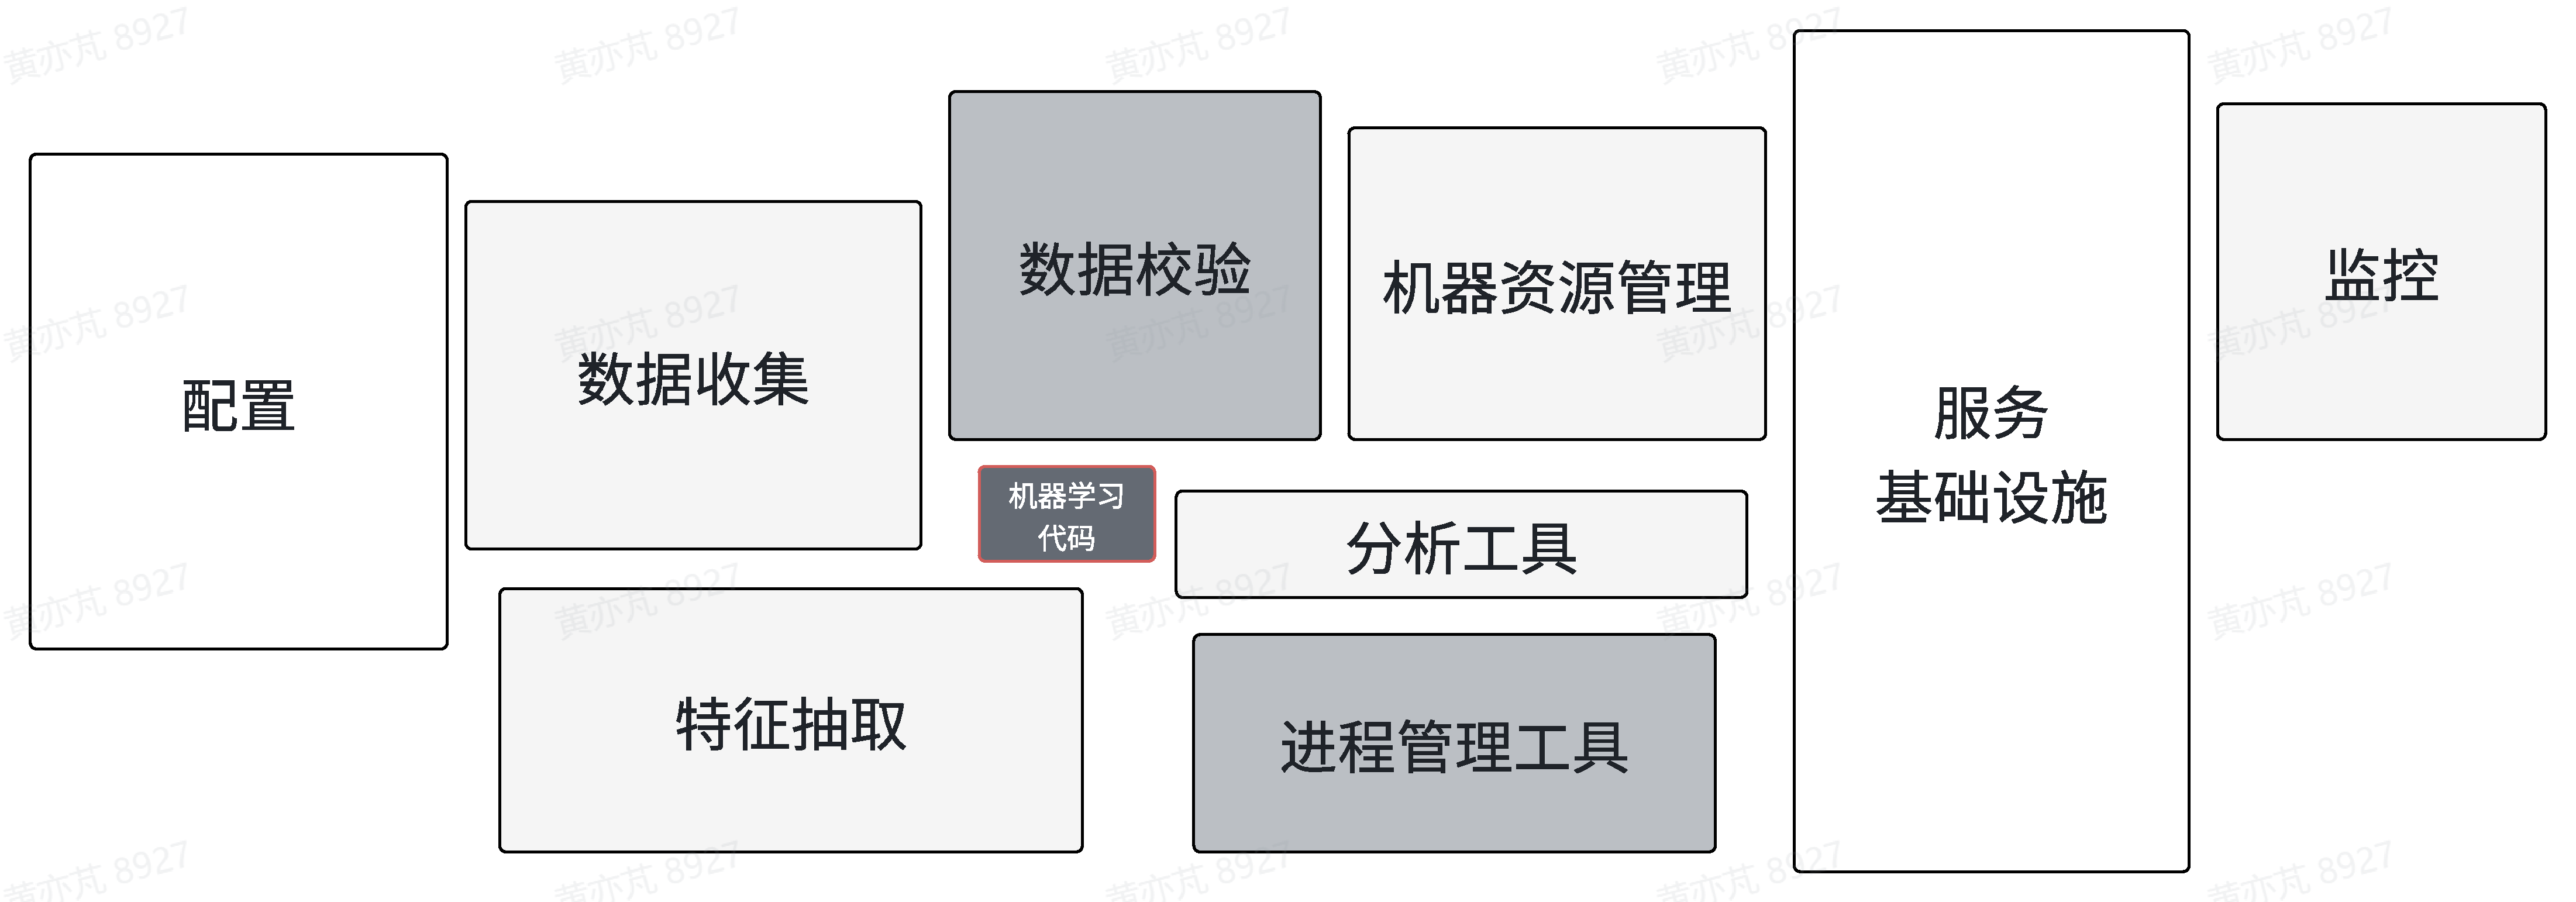
\includegraphics[width=0.98\linewidth]{ml-system-components.pdf}
  \caption{谷歌提出的机器学习系统组成}
  \label{fig:mlcomponents}
\end{figure}

人类的技术发展总是伴随着工程化的进程:从人力种植到机械耕作、从手工制造到工业生产、从编程开发到软件工程等等。
其中的关键是工具手段的出现和演进以及流程的标准化和自动化,以支撑技术的规模化应用。
其核心就是提高生产效率,从而解放生产力,降低生产成本,提高产品质量。
在机器学习领域,工程化的进程也是必然的,也是迫切的。
正如谷歌在机器学习系统设计的奠基性理论研究中所提出的,真实世界的机器学习系统中包含广阔而复杂的工程化基础设施,机器学习代码只是系统中很小的一部分,如图\ref{fig:mlcomponents}。
在模型核心技术研发的层面上,数据准备、算法开发、模型训练、模型评估等环节需要工具手段的辅助,以提高研发效率和模型性能;
在模型应用落地的层面上,模型部署、模型监控、流程自动化、业务应用集成等环节更需要工程化的系统软件支撑,以保证应用的稳定性、可靠性和可维护性。

【与软件工程的不同】
模型结构复杂、训练数据多、参数量大、随机性强

【为什么云原生】

需要注意的是,一些文献中将PyTorch、TensorFlow等机器学习计算框架称为机器学习平台,易与本文的研究对象混淆。
本文研究的机器学习平台是指支撑机器学习研发和应用的软件工具系统,依托于硬件基础设施(或称硬件平台,亦与本文中的平台不同),支持在平台中使用PyTorch、TensorFlow等机器学习计算框架进行模型训练、推理等计算作业。


%
\section{国内外研究现状}

TBD

\subsection{理论方法}

在实际的研发工作当中,模型开发过程难复现、实验程序难复用等问题频繁出现,导致大量的重复劳动,研发可持续性较差. Fursin等人\cite{Fur16}提出了一套模型研发产出的标准框架,规定了环境、算法、程序、流水线等相关内容的定义方式,研发人员可基于此形成研发项目数据库,支撑研发过程中产生的组件、工具、流程的复用,为团队协作提供基础,进而保障研发的可持续性. 

\subsection{系统研究}

针对机器学习应用落地的难题,一些研究工作体现在端到端的机器学习平台上\cite{Bay17, Sal18},机器学习模型的研发只是其中的一个环节。
平台的功能覆盖数据、模型训练和验证、应用部署和监控等方面,期望打通从数据接入到业务应用运维的机器学习完整工作流\cite{Ame19},满足机器学习应用快速上线并形成稳定服务的需求。
追求落地固然是机器学习技术的主要目标,但从根源上,如何使机器学习研发更高效是亟待突破的首要方向,将会对应用落地带来诸多裨益。

Kumar等人\cite{Kum16}将传统机器学习的模型开发过程抽象成特征工程、算法选择和参数调优等3项关键步骤,统称为“模型选择”(Model Selection),并基于此概念提出一种模型选择管理系统框架,包括声明式实验构建、运行时计算优化、模型来源管理与分析等功能,支撑高效的机器学习实验。
Tsay等人\cite{Tsa22}提出了人工智能实验数据库,着重针对研发过程可复现性问题,通过对实验元信息的建模、抽取和关联,聚焦实验产物及其生成过程的完整详细信息,保障从数据处理到模型实验的复现。
同样在研发过程方面,Sridhar等人\cite{Sri18}提出了模型治理的概念及相关系统,覆盖了机器学习模型开发与部署中的模型血统梳理、可复现性、审计、伸缩等需求,旨在帮助研发人员明确模型的产生路径及其在生产环境中的用途和效果,从而更好地复现研发方案、诊断实验过程中存在的问题。

模型是机器学习研发阶段最核心的产物,模型管理的重要性不言而喻. 模型管理系统在不同领域、不同应用场景下面临着诸多挑战\cite{Sch15, Scu15},近年来得到了学术界的广泛关注。
Vartak等人\cite{Var16}提出一种模型管理系统,以代码侵入的方式对实验进行跟踪,并对模型进行统一存储和索引,为用户提供共享、查询、分析等功能,帮助研发人员梳理模型研发过程、找寻规律并建立整体视角。
Schelter等人\cite{Sch17}则提出一种非侵入式模型跟踪方法,可针对一些机器学习框架自动进行实验记录,并提取出数据集、超参数、模型等机器学习常见资产的元信息,支撑实验的对比和复现以及模型血统分析。
Miao等人\cite{Mia17}针对深度学习模型研发提出了一套模型生命周期管理平台,更多地关注了模型快速迭代过程中的版本控制以及模型的社区式共享机制,并搭配了一种领域专用语言用以高效地检索和查询平台中的模型资产。
此外,该平台内置了一套模型来源管理模块,以图数据库的形式帮助用户记录、管理和梳理深度学习模型开发的过程。

\subsection{平台产品}

产业界近些年也涌现了一批实验跟踪与模型管理的系统或平台\cite{wandb, neptuneai, huggingface},在模型资产管理和团队协作上的实践经验对模型研发管理系统的学术研究具有指导意义。

\subsection{小结}

上述相关研究工作普遍在算法管理、计算环境管理、研发团队分工协作、实验方案的细粒度跟踪等方面存在不足之处:
(1)现有系统往往将机器学习算法视为传统软件代码,全权交由用户以通用的代码管理系统(例如GitHub)进行管理,缺乏对算法的资产化管理,进而无法有效地与模型、数据集等其他机器学习核心资产形成有机关联;
(2)同样地,现有系统也缺乏对计算环境的资产化管理,难以保证多次计算任务中环境的一致性;
(3)团队协作被广泛纳入现有系统的功能板块中,但往往仅限于团队成员间的资源共享机制,缺乏团队的组织架构管理以及任务的分工指派;
(4)类似地,实验跟踪虽然是现有系统的基本功能,但一般只能跟踪算法代码的提交信息,在探索式、迭代式的模型调试过程中,用户往往不会对每次细微的改动均做提交,现有系统便无法完整跟踪到每一次的方案变更。
本文提出的Anylearn机器学习研发管理系统在资产管理、团队协作、研发过程跟踪的功能框架下,研究并解决了相关工作存在的这些问题.


%
\section{研究内容与主要贡献}

针对机器学习研发过程中存在的工作流程缺乏顶层设计、资产缺乏统一管理等研发管理问题,本文从工程化的角度出发,在体系架构、关键技术和系统设计实现等方面研究如何构建一套云原生机器学习平台,为模型研发团队输出体系化、标准化、规模化的机器学习研发作业和管理能力,并提供覆盖数据开发、模型开发、模型训练、模型调整、模型部署、模型服务等机器学习研发生命周期核心环节的工具手段,提高研发效率和模型性能,为机器学习应用落地提供有力支撑。

本文的主要贡献有以下几方面:
\begin{itemize}
  \item 在体系架构方面,本文按照能力体系、功能体系、数据体系、技术体系和交互体系五个维度展开论述,逐级细化剖析机器学习平台的形态,明确平台的能力边界和组成关系,为平台的设计和实现提供指导;
  \item 在关键技术方面,本文从云原生系统相关技术和机器学习相关技术两个角度进行研究,分别探讨了云原生系统的容器化、资源池化、存储等技术在机器学习平台中发挥的作用和应用价值,以及机器学习模型的训练、调优、部署等方面的核心技术点的背景问题和技术原理;
  \item 在系统设计方面,本文提出了Anylearn大数据机器学习研发管理系统的设计方案,并阐述了实际线上长活环境的运行情况和真实科研用户的使用案例,验证了系统的可行性和有效性。
\end{itemize}


%
\section{本文结构安排}

本文围绕研究内容的体系架构、关键技术和系统实现三方面进行论述,后续章节安排如下:第2章研究机器学习平台的体系架构,包括能力体系、功能体系、数据体系、技术体系和交互体系;第3章研究机器学习平台的关键技术,包括云原生系统相关技术和机器学习相关技术;第4章研究机器学习平台的系统设计实现,包括Anylearn大数据机器学习研发管理系统的使用场景、系统设计、线上环境运行情况和用户使用案例;第5章总结全文,展望未来工作。  

% !TeX root = ../thuthesis-example.tex

\chapter{机器学习平台体系架构}

\section{总体架构}

围绕Google的ML系统技术债,描述机器学习平台内部的大致组成以及外部的交互关系。
TBD


\section{能力体系}

TBD


\section{功能体系}

TBD


\section{数据体系}

TBD


\section{技术体系}

TBD


\section{交互体系}

TBD

% !TeX root = ../thuthesis-example.tex

\chapter{云原生背景下的相关技术}

简述云原生技术背景,云原生应用开发范式,Kubernetes作为云原生的事实标准……
TBD


\section{容器化机器学习}

TBD


\section{计算资源池化}

TBD


\section{分布式存储}

TBD


\section{分布式训练引擎}

人工智能是如今计算机领域发展迅猛的一个方向,尤其是大模型的横空出世及其应用展现出的强大能力,给未来带来了无限的想象空间。

在大模型大放异彩的背后,大模型的训练是一个复杂的大规模系统工程,涵盖了机器学习理论、计算机系统结构、分布式计算和软件工程等多个计算机科学研究领域。
大模型的训练可以视为大规模的分布式训练,往往需要用到几十到上千台机器(后文的机器指的是带有GPU的AI服务器)协同工作数十天。
本节着重介绍云原生场景下分布式训练的相关技术。

\subsection{背景问题}
如今,许多相关工作者正在致力于优化和加速大模型的训练过程,大模型训练涉及的技术栈较多,主要可以划分为以下三个层次:硬件层、框架层和平台层。
其中,AI平台能够提供数据处理、模型训练、模型推理等服务,管理和调度整个集群的资源,与底层机器交互并进行集群运维,使得用户不需要关心机器硬件方面的问题,能够专注于算法层面上的研究。
因此,平台的功能是否完善、是否能帮助算法工程师减少不必要的时间浪费,对提升模型训练效率至关重要。

由于AI平台会面向很多用户,并且肩负着大规模分布式机器资源管理的职责,因此,AI平台通常会和适用于大规模优化的“云计算”技术紧密关联。
同时,随着云计算的发展逐渐成熟,业界出现了云原生分布式训练的相关技术。
云原生充分利用了云计算提供的基础资源和弹性伸缩的能力,能够构建迭代速度更快、资源利用率更高、容错能力更强的应用程序。
分布式训练是AI平台必须具备的功能,换言之,AI平台需要支持大参数量模型的训练。
此外,当前市场上的算力是十分昂贵的。
例如,一张NVIDIA A100每月的租赁价格大约16000元。
在大规模的分布式训练过程中有机器发生故障的频率会随着机器数量的增长而大幅度增加。
因此分布式训练会经常出现因为机器故障导致训练任务失败的情况,不仅会导致训练开发效率降低,而且会导致大量的时间与金钱的浪费。
为解决上述问题,AI平台具有为分布式训练提供运行保障的能力也非常关键,例如自动重启失败的训练、自动检测GPU是否存在故障、提供方便调试的途径等。

\subsection{分布式训练技术}
分布式训练是一种通过多个分布式的AI服务器计算节点协同工作以加速机器学习模型训练过程的技术。
分布式训练能够有效利用并行计算的优势,通过将大型计算任务分解成若干子任务,并将这些子任务分配到多台机器上执行,从而缩短训练时间,提升训练效率。
下面将从分布式训练的并行策略、通信操作以及目前主流机器学习框架开展研究分析。

分布式训练的核心问题是:数据和模型如何分配到不同的计算节点上,各个节点上的计算结果又如何汇总,才能更有效地缩短训练时间,提升训练效率。
针对该问题,国内外研究学者分别在并行策略和通信操作两方面做了大量研究工作。
当前分布式训练的并行策略主要研究并行计算的模式,目前常见的并行策略主要有以下几类:

(1)数据并行(Data Parallelism)思想早在并行计算兴起初期就已出现,在机器学习兴起之后,也自然而然地移植到了分布式训练之中。
具体方法是将大数据集分割成多个小数据批次,每个计算节点独立处理一个批次的数据,并在所有节点上共享模型参数,各个节点通过梯度平均化或类似的方法同步模型更新。

(2)模型并行(Model Parallelism)是将大型模型划分为多个部分,每个计算节点负责模型的一部分。
节点之间通过特定的通信机制交换中间结果,共同更新整个模型的参数。其中,Megatron就主要参考了模型并行的思想。

(3)流水线并行(Pipeline Parallelism)是模型并行的改进版本,将模型的训练过程按层或阶段划分,形成一个流水线式的处理流程,每个节点专注于模型的一部分并在节点间传递中间结果。
目前有在机器学习框架中实现流水线并行的工作,如GPipe。

(4)参数服务器架构(Parameter Server)是将集群的一个或多个节点作为中心化的参数服务器,用于存储和管理模型参数,其他节点则负责计算并上传梯度,参数服务器接收到梯度后更新模型参数,然后再分发给参与训练的其他节点。
这一架构的缺点在于参数服务器的数据传输量非常巨大,因此现在已经较少使用。

(5)混合并行策略则是结合了数据并行、模型并行和其他技术,以适应更加复杂的训练场景和资源分配需求。
特别是在大模型的训练中,开发者通常不会单一地使用某种并行计算模式,而是手动设计并行方式。
图\ref{fig:disttraining}展示了一种同时采取了模型并行和数据并行的分布式并行策略,将 256 张 GPU 分成 32 组,每组内的 8 张GPU做模型并行,同时 32 组之间进行数据并行,从而实现数百张GPU的分布式训练。

\begin{figure}
  \centering
  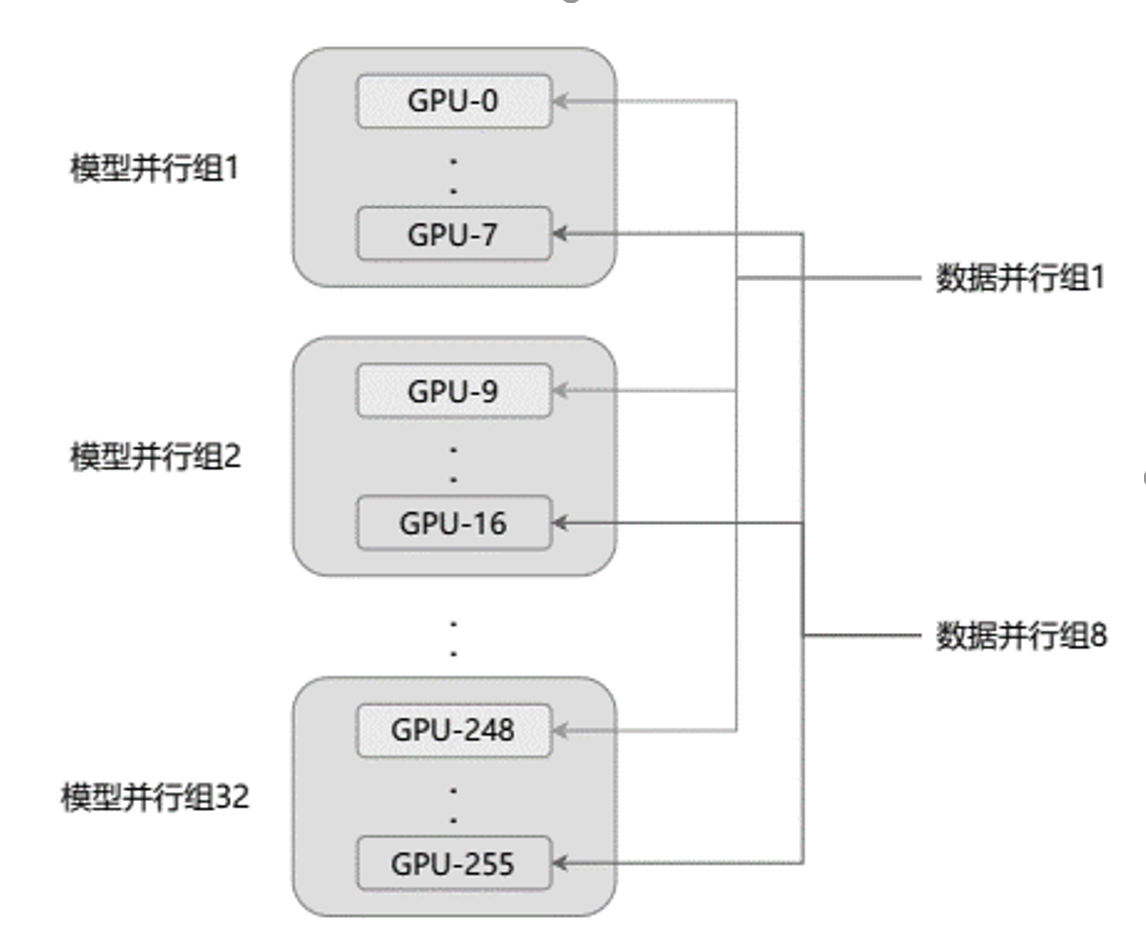
\includegraphics[width=0.6\linewidth]{dist-training.png}
  \caption{分布式训练混合并行策略示意}
  \label{fig:disttraining}
\end{figure}

分布式训练中会涉及节点之间的通信操作,通信操作指的是在多个计算节点之间交换信息,以确保模型训练过程中的数据一致性、梯度同步和参数更新的过程。
常见的分布式通信操作如下:

(1)Scatter(散播)操作是指将一个大的数据集或模型参数分割成多个部分,并将这些部分均匀地分配到不同的计算节点上,每个节点独立处理自己分得的那一部分数据或参数。

(2)Reduce(归约)操作是将分布在多个节点上的相同类型的数据通过某种操作聚合到一起,得到一个全局的结果。
例如,在深度学习训练过程中,各个节点各自计算出局部梯度后, Reduce 操作会将所有节点上的梯度累加起来,得出整个模型的全局梯度。

(3)AllReduce 操作整合了 Scatter 和 Reduce 操作,并将归约后的结果同步到所有参与计算的节点上。
在分布式训练中, AllReduce 对数据并行的训练十分重要,能够确保所有节点在一轮迭代结束后拥有相同的模型参数更新值。

(4)Ring AllReduce是AllReduce的优化版本,其特点是利用环形网络拓扑来进行数据交换和归约操作。
在 Ring AllReduce中,每个节点仅与其相邻的两个节点进行通信,形成一个环状结构。
整个过程分为若干轮次,每一轮中每个节点向其右侧节点发送一半数据,并从左侧节点接收另一半数据,同时在接收过程中对收到的数据与本地数据进行相应的运算。
通过这种方式,所有节点逐步累积并更新数据,直到所有节点都获得了完整的全局运算结果。
Ring AllReduce的通信成本复杂度较低,在大规模GPU集群中特别受欢迎,大大提高了分布式训练的效率和可扩展性。

\subsection{主流机器学习框架}

机器学习框架是指一种专门设计的软件开发工具包或平台,为开发者提供了标准化的接口、模块化组件和预先实现的算法集合,以支持机器学习模型的快速开发、训练、验证、优化以及部署。
常见的机器学习框架有PyTorch、TensorFlow、MXnet、Caffe、Xgboost等,其中PyTorch是目前使用人数最多的机器学习框架,框架中对分布式训练也有支持。

\subsection{云原生分布式训练}

云原生是一种构建和运行应用程序的方法论,充分利用了云计算的弹性和可扩展性,结合现代化的软件开发实践,确保应用程序能够在公有云、私有云和混合云环境中无缝运行和高效管理。
云原生包含的关键技术有容器技术、容器编排系统、微服务治理工具、DevOps工具链等。

Kubernetes是目前最流行的实现云原生理念的容器编排系统,是开发云原生应用的关键基础设施。
从功能角度出发,Kubernetes系统可以大致分为管控和资源两大部分:管控部分涉及Kubernetes系统的管理和资源的控制功能,通常由系统中持续运行的组件完成。
资源主要指系统中被管理和调度的对象,有更新较频繁、具有动态性质的资源(如Pod),也有在系统中长期存在、相对静态的资源(如自定义资源CRD)。
在实际实现分布式训练时,需要用到一些别的组件和资源。
分布式涉及到相关组件和资源的架构如图\ref{fig:disttrainingk8s}所示。

\begin{figure}
  \centering
  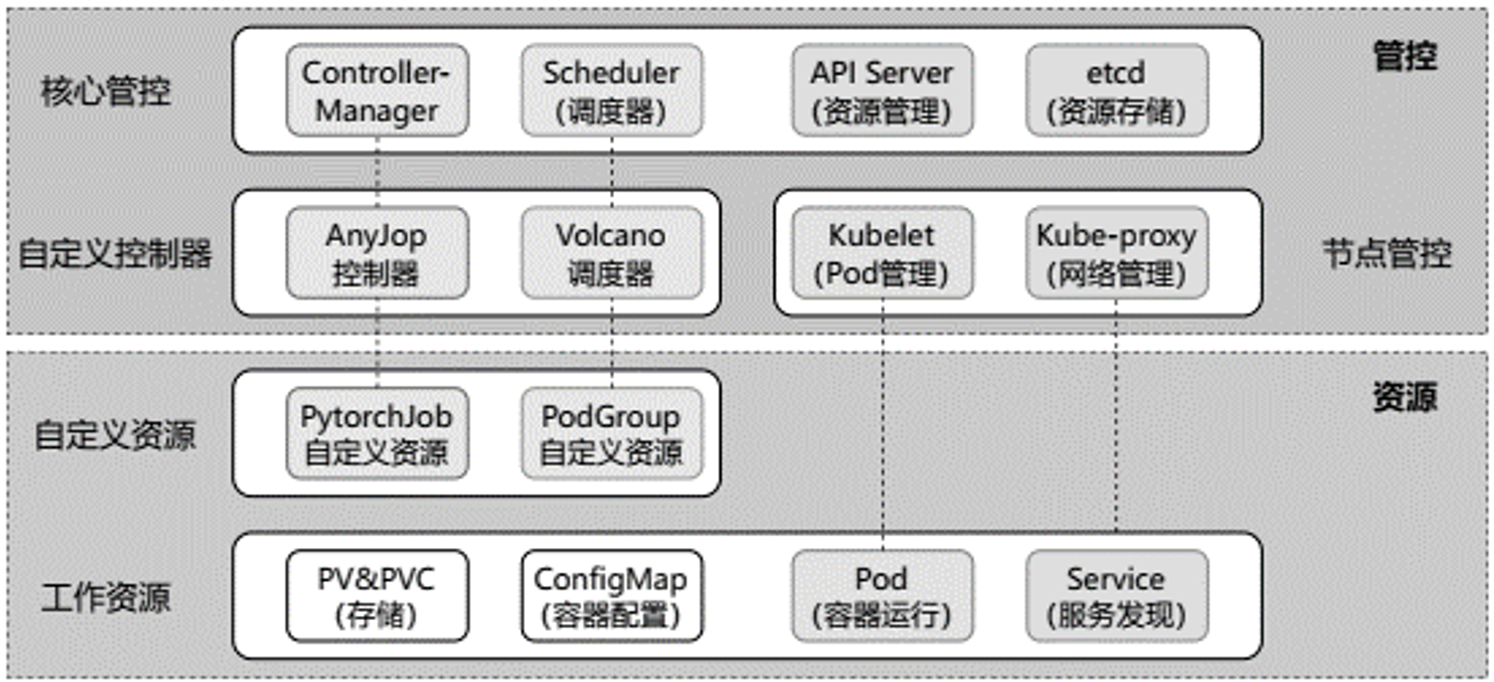
\includegraphics[width=0.8\linewidth]{dist-training-on-k8s.png}
  \caption{云原生分布式训练引擎基础架构示意}
  \label{fig:disttrainingk8s}
\end{figure}


\section{训练过程数据跟踪与可视化}

对于机器学习模型研发而言,训练过程的数据跟踪与可视化是非常重要的环节,能够帮助开发者更好地理解模型的训练过程,发现模型训练中的问题,提高模型的训练效率。
本节就训练过程数据跟踪与可视化的相关技术进行介绍。

\subsection{背景问题}

随着数据量和计算能力的不断提升,机器学习模型的训练过程变得更加复杂和耗时。
训练过程中的数据量大、计算密集度高,导致训练任务的管理和优化成为一项重大挑战。
当前,许多研究团队面临以下几个问题:

\textbf{(1)训练过程监控困难}

在深度学习模型的训练过程中,实时监控模型指标(如损失、准确率、梯度、权重等)对于研究人员来说至关重要。
这些数据能够帮助研究人员及时了解模型的训练状态,从而判断模型是否存在过拟合、欠拟合或训练效率低下等问题,并据此调整训练策略,优化模型性能。

目前,许多研究团队使用TensorBoard等开源工具来实现训练过程的监控。
TensorBoard提供了基本的可视化功能,但在某些方面存在局限性。
其中最显著的是,TensorBoard的多任务对比功能有限,它只允许对比同名指标,缺乏灵活性。
在实际研究中,研究人员常常需要对比不同模型或任务的多种指标,这就使得TensorBoard的功能显得不够灵活。

此外,TensorBoard的面板(panel)是固定的,用户无法根据不同任务和需求自定义面板。
这导致研究人员在需要展示特定指标组合时,往往需要下载数据并通过其他工具手动绘图,这无疑增加了操作的复杂性和工作量。
例如,假设研究人员正在同时训练两个模型,他们可能希望对比两个模型的准确率和损失。
但由于TensorBoard的多任务对比功能有限,他们可能无法直接在同一个界面中对比这两个指标。
他们可能需要打开两个不同的TensorBoard窗口,分别查看两个模型的指标,这样的操作显然不够便捷。
同样,如果研究人员希望自定义一个面板,以展示特定指标的组合,他们也将面临困难。
由于TensorBoard的面板是固定的,他们无法根据自己的需求来定制面板。
他们可能需要将数据导出到其他工具,如Matplotlib,然后手动绘制图表,这无疑增加了工作量。

总的来说,尽管TensorBoard是一个强大的可视化工具,但在多任务对比和自定义面板方面,它还存在一些局限性。
研究人员需要寻找其他工具或方法来满足这些需求。

\textbf{(2)数据分散管理}

在深度学习模型的训练过程中,数据的多样性和分散性带来了管理上的挑战。
训练过程中会产生多种类型的数据,如训练日志、模型权重、评估指标和训练数据等,这些数据通常分散存储在本地文件系统、远程服务器和云存储等多个位置。
这种分散管理的方式导致了数据读取效率低下,研究人员在分析和处理数据时需要频繁地在不同存储位置之间切换,从而增加了时间成本。
同时,数据一致性问题也随之产生,因为分散存储的数据可能会在不同位置出现版本不一致的情况,这会给研究人员在分析数据时带来困扰。

此外,数据的安全和隐私保护也面临着更大的挑战,因为数据存储在不同的位置,增加了泄露和丢失的风险。
缺乏集中管理的机制使得数据的安全性和隐私性难以得到有效保障。
在团队协作方面,分散的数据管理也增加了协同工作的难度,团队成员在需要访问和处理相同数据时,数据的传输和共享变得复杂,这影响了团队的整体工作效率。

为了解决这些问题,亟需开发一个高效的训练过程监控与数据管理系统,以克服现有工具的局限性。
这样的系统将实现数据的集中管理和高效处理,提升模型训练的管理和优化效率,同时确保数据的安全性和隐私保护,简化团队协作流程,从而推动研究工作的顺利进行。

\subsection{训练过程跟踪系统架构}

系统主要由交互层、业务层和存储层三个部分组成,如图\ref{fig:anyboardarch}所示。

\begin{figure}
  \centering
  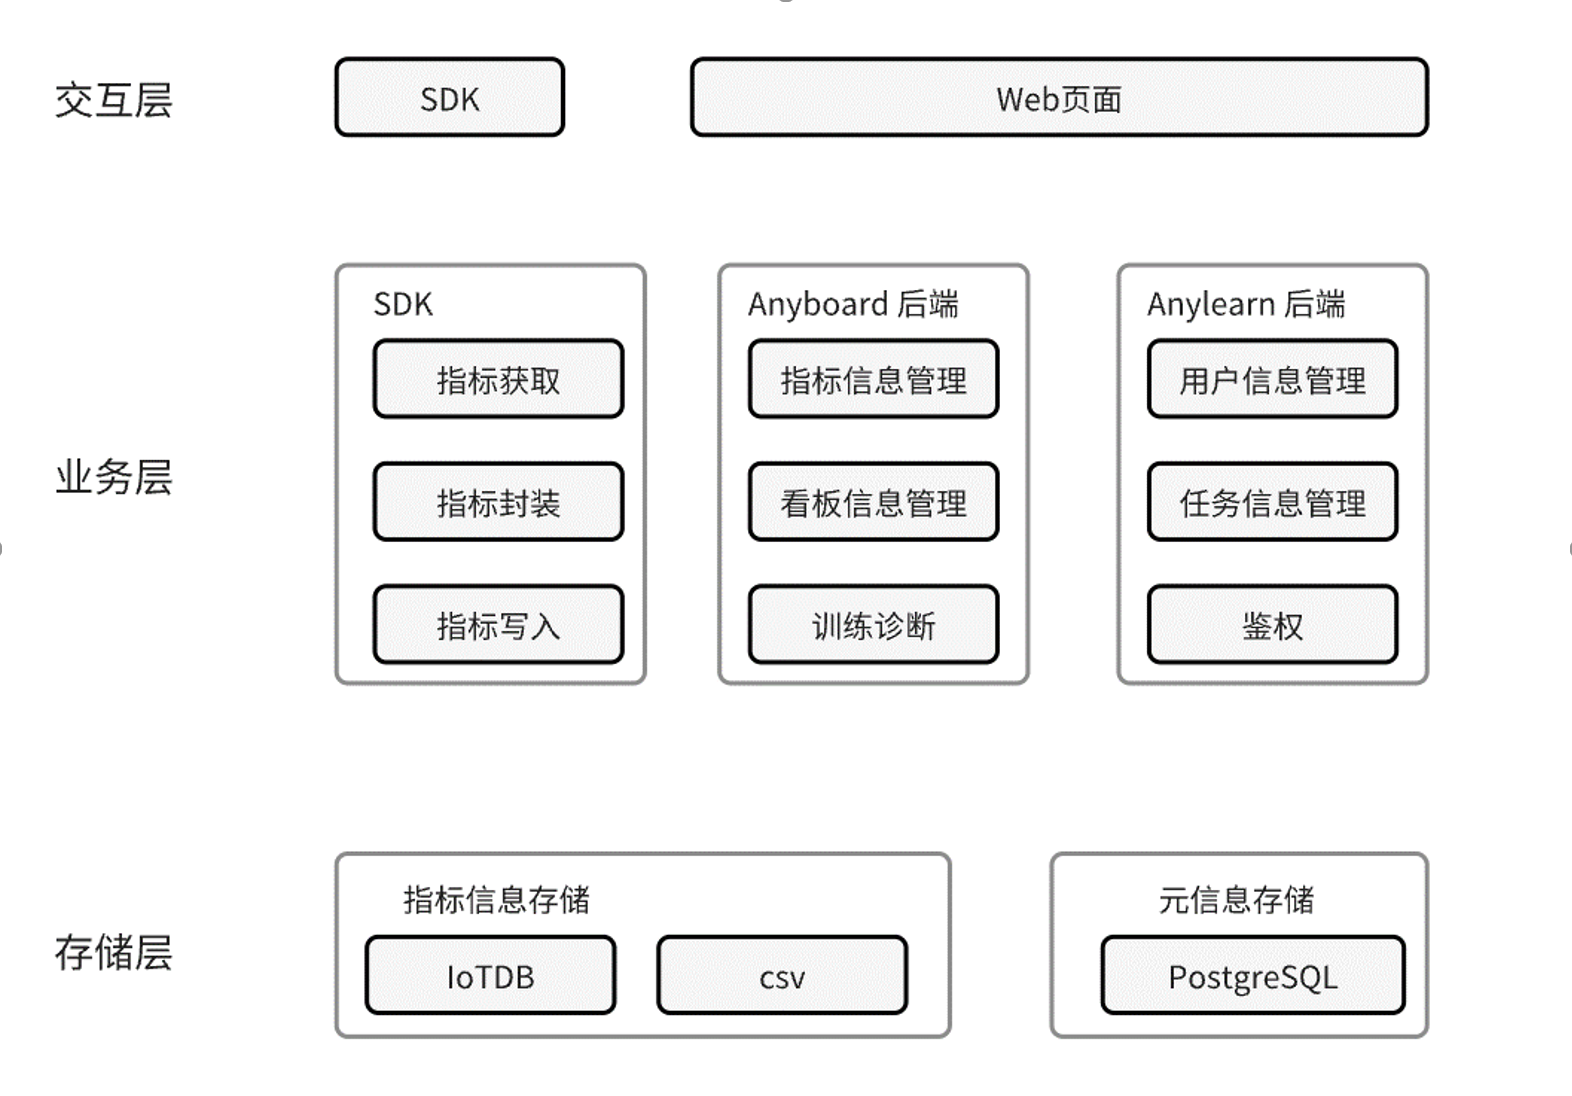
\includegraphics[width=0.8\linewidth]{anyboard-architecture.png}
  \caption{训练跟踪与可视化系统架构}
  \label{fig:anyboardarch}
\end{figure}

(1)交互层:首先,SDK作为编程接口,使用户能够在代码中直接记录训练过程中的各种指标数据。
它提供了方便的API,支持多种指标类型的记录,如标量、图片、直方图等。
通过SDK,用户可以在训练过程中方便地收集和记录所需的指标数据,以便后续分析和优化。
其次,Web页面通过直观的界面与用户交互,提供指标的实时可视化功能。
用户可以在Web页面上查看和分析训练过程中记录的各种指标数据。
Web页面将指标数据以图表、图像等形式展示给用户,使用户能够更直观地了解训练过程,发现潜在问题,并进行相应的调整和优化。
用户可以在Web页面上查看和分析训练过程中记录的各种指标数据。

(2)业务层:首先,指标记录功能处理用户通过SDK传入的指标数据。
当用户在代码中记录训练指标时,SDK将这些数据转换为标准格式,以确保数据的统一性和可处理性。
随后,这些标准格式的数据会被存储到后端数据库中,以便于长期保留和分析。
其次,指标管理功能负责管理和维护指标数据。
这包括创建新的指标数据记录、更新现有指标数据的值以及删除不再需要的指标数据。
指标数据的元信息,如指标名称、类型、单位等,也会被一同管理和维护,确保数据的准确性和完整性。
接着,指标展示功能提供实时数据查询和展示服务。
它将存储在数据库中的指标数据通过可视化的方式呈现给用户,例如以图表、曲线图或直方图的形式。
这样的展示方式帮助用户直观地理解训练过程,包括模型的性能变化、训练速度等关键信息。
最后,训练诊断功能基于记录的指标数据,对训练过程进行分析,以识别可能的异常情况。
它提供实时的诊断服务,帮助用户快速定位和解决问题。
例如,如果发现训练过程中的性能指标突然下降,诊断工具可以帮助用户分析造成这种情况的原因,是数据问题、模型结构问题还是学习率设置不当等。

(3)存储层:IoTDB时序数据库\cite{Wan23}专为存储时间序列数据设计,它在训练过程中用于收集和存储大量的时间序列数据。
时间序列数据是指按时间顺序记录的数据点集合,常用于监控系统性能、日志记录、气象数据等。
IoTDB支持高效的数据插入和查询操作,能够处理高频率、大规模的数据流,非常适合于训练过程中产生的海量时间序列数据的存储和管理。
IoTDB的特性包括数据压缩、数据索引、时间范围查询等,这些特性能够提高数据存储的效率和查询的速度。
CSV文件则适用于存储小规模离线训练任务的指标数据或作为数据文件的备份。CSV(Comma-Separated Values)文件格式是一种简单的文本文件格式,其中数据以行和列的形式存储,每列之间的分隔符通常是逗号。
CSV文件格式易于读取和处理,可以使用多种编程语言和工具进行数据的读取和分析。
对于小规模的训练任务,使用CSV文件存储指标数据可以快速方便地存取数据,而不需要复杂的数据库管理系统。
PostgreSQL是一种功能强大的关系型数据库,它用于存储训练过程中的元数据。元数据包括用户信息、项目信息和看板配置信息等。
这些信息通常是结构化的,需要进行复杂查询和事务处理。
PostgreSQL支持SQL查询语言,提供了高级的数据管理和操作功能,如数据完整性约束、视图、索引等。
使用PostgreSQL存储元数据可以确保数据的安全性、完整性和一致性,同时也便于进行复杂的数据分析和报告。

\subsection{端云协同的指标跟踪机制}

在端侧,通过SDK接口,用户可以在训练代码中直接记录指标数据,这极大地方便了数据的收集,并确保了数据记录的实时性和准确性。
同时,端侧的Web页面提供了直观的交互界面,使得用户能够实时查看训练指标,并通过图表等形式进行数据分析。

在云侧,采用了专业的时序数据库IoTDB来存储大量的时间序列数据,确保了数据的高效存储和快速检索。
此外,使用PostgreSQL数据库存储结构化元数据,提供了数据的安全性和复杂查询的支持。
云端的存储解决方案,不仅支持大规模数据的处理,还可以通过远程访问,实现数据的集中管理和分析。

系统的端云协同工作模式,允许用户在本地进行实时的数据监控和诊断,云端则负责长期的数据存储、分析和复杂查询。
这种工作模式使得用户能够充分利用本地资源进行快速开发和调试,同时又能够享受到云端强大数据处理能力和分析服务。
例如,当训练过程出现异常时,系统不仅能够实时检测到异常,还能够通过云端的大数据分析,为用户提供针对性的解决方案。

\subsection{实时数据展示与诊断}

实时数据展示与诊断是深度学习训练过程中的重要环节,它通过前端看板和相应的分析功能,使用户能够实时监控训练进度,快速识别和解决问题。

前端看板是实现训练指标实时可视化的界面。
它利用Vue框架和Echarts库,将训练过程中的各类指标以图表、曲线图、柱状图等形式展示给用户。
这些可视化元素使得训练过程中的复杂数据变得直观易懂,用户可以实时关注到模型的性能变化、训练速度、资源消耗等关键指标。
自定义面板功能允许用户根据不同任务的需求,灵活创建和配置看板。
用户可以根据自己的关注点,选择展示特定的指标,或者按照任务类型进行指标分类。
此外,自定义面板还支持多任务对比,帮助用户分析不同模型或任务的训练效果,从而做出更合理的决策。

训练诊断功能包括异常检测和问题解决建议两个部分。
异常检测是基于记录的指标数据,对训练过程进行实时分析,以发现可能的问题。
例如,系统可以检测梯度异常、损失变化异常等,这些异常可能是模型过拟合、学习率设置不当等原因造成的。
系统提供实时的诊断功能,帮助用户快速发现和定位这些异常。当检测到异常时,系统会提供相应的解决建议。
这些建议基于训练过程中的数据分析,旨在帮助用户及时调整训练策略,优化模型性能。
例如,如果检测到梯度消失问题,系统可能会建议尝试调整学习率或使用更合适的优化器。
通过上述技术原理,系统实现了对训练过程的高效监控和数据管理,解决了现有工具的局限性,显著提升了训练任务的管理和优化效率。


\section{超参数高效调优}

超参数调优往往对机器学习模型的效果起着决定性的作用,在模型应用落地时至关重要。
本节就高效超参数调优技术进行介绍。

\subsection{背景问题}

深度神经网络(DNN)在许多应用中取得了显著的成功,特别是在图像识别、自然语言处理、语音识别等领域。然而,DNN的性能高度依赖于超参数的选择,合理的超参数设置能够显著提升模型的表现。然而,传统的超参数调优方法面临以下几方面的挑战。

(1)超参数组合多:深度神经网络(DNN)的超参数种类繁多,包括学习率、批量大小、网络层数、每层的神经元数量、激活函数的选择、正则化参数等。
每种超参数都有多个可能的取值,例如,学习率可以是0.001、0.01或0.1,批量大小可以是32、64或128,网络层数可以是3层、5层或10层,激活函数可以选择ReLU、Sigmoid或Tanh,正则化参数可以是L2正则化、Dropout等。
由于每个超参数的可能取值都不同,所有可能的组合数量呈指数增长。
例如,如果有6种超参数,每种超参数有3个可能取值,组合数将是3的6次方,即729种组合。
这种组合数量随着超参数数量和每个超参数的取值范围的增加而迅速增长,使得全面搜索所有可能的超参数组合变得几乎不可能。
此外,实际应用中,为了获得最优的DNN模型,往往需要尝试更多种类的超参数及其更多的取值,这进一步增加了组合数量的复杂性和计算量,给传统的超参数调优方法带来了巨大挑战。
这种组合爆炸现象严重影响了超参数调优的效率和效果,导致计算资源浪费和调优过程的冗长。

(2)训练耗时长:每次对超参数组合的评估都需要进行完整的训练和验证过程,这在大规模数据集和复杂模型结构下尤为耗时。
深度神经网络通常包含数百万甚至数十亿个参数,这些参数需要通过反复的前向传播和反向传播来优化。
对于大型数据集,每次训练迭代都需要处理大量的数据,这使得训练时间大幅增加。
此外,复杂的模型结构,如深度较大的卷积神经网络(CNN)或包含大量节点的循环神经网络(RNN),需要更多的计算资源来完成每次迭代。
因此,训练一个模型可能需要数小时、数天甚至数周的时间。
当进行大规模的超参数调优时,需要对大量不同的超参数组合进行试验,每个组合都需要完整的训练和验证过程,这进一步加剧了耗时问题。
这种大规模的训练需求耗费了大量的计算资源和时间,严重限制了调优效率。
即使使用高性能计算设备,如GPU或TPU,加速效果也有限,因为每次超参数调整都需要重新开始训练过程。
由于超参数空间巨大,传统的网格搜索或随机搜索方法需要尝试数百甚至数千种组合,这使得超参数调优过程变得异常缓慢和昂贵,无法快速找到最佳的超参数组合,从而影响了模型性能的优化。

(3)训练过程随机性大:深度神经网络(DNN)的训练过程具有高度的随机性,这源于多个方面的因素。
首先,权重初始化的随机性在训练开始时就引入了不确定性,不同的初始化可能导致模型收敛到不同的局部最优解。
其次,数据的随机分批处理(mini-batch)在每个训练迭代中使用的数据子集是随机选择的,这种随机选择会影响模型参数的更新路径。
此外,优化算法中的随机性,如随机梯度下降(SGD)及其变种(如Adam、RMSprop),在每次参数更新时都会引入随机噪声,从而影响模型的收敛过程。
这些随机因素的综合作用导致同一组超参数在不同的训练过程中可能得到显著不同的结果,表现为模型性能的波动。
这种结果的不一致性增加了超参数调优过程的不确定性和难度,因为无法确定某次试验结果的优劣是由超参数本身决定的,还是由训练过程的随机性导致的。
为了克服这些随机性影响,需要多次重复试验并取平均值或最优值来评估超参数组合的性能,这进一步增加了计算成本和时间开销。
随机性的存在还使得超参数调优结果的可重复性和稳定性降低,使得调优过程变得更加复杂和耗时。

这些问题严重影响了DNN超参数调优的效率和效果。
传统方法如网格搜索(Grid Search)和随机搜索(Random Search)虽然简单直观,但面对高维度超参数空间和训练时间长的问题时显得无力。
针对这些挑战,需要开发新的技术手段,以更高效、更精准地进行超参数调优,从而提升深度神经网络的性能和应用价值。

\subsection{基于训练诊断的超参数调优}

为了应对上述挑战,学界提出了一种基于训练时学习过程质量指标的超参数调优方法\cite{Pei24}。
该方法的核心思想是通过实时监测和评估训练过程中的质量指标,提前停止那些表现不佳的超参数组合试验,节约计算资源并将其用于更有潜力的组合。

技术架构如图\ref{fig:anytunerarch}所示,主要包括指标监测模块、质量评价模块和资源调度模块三个部分。

\begin{figure}
  \centering
  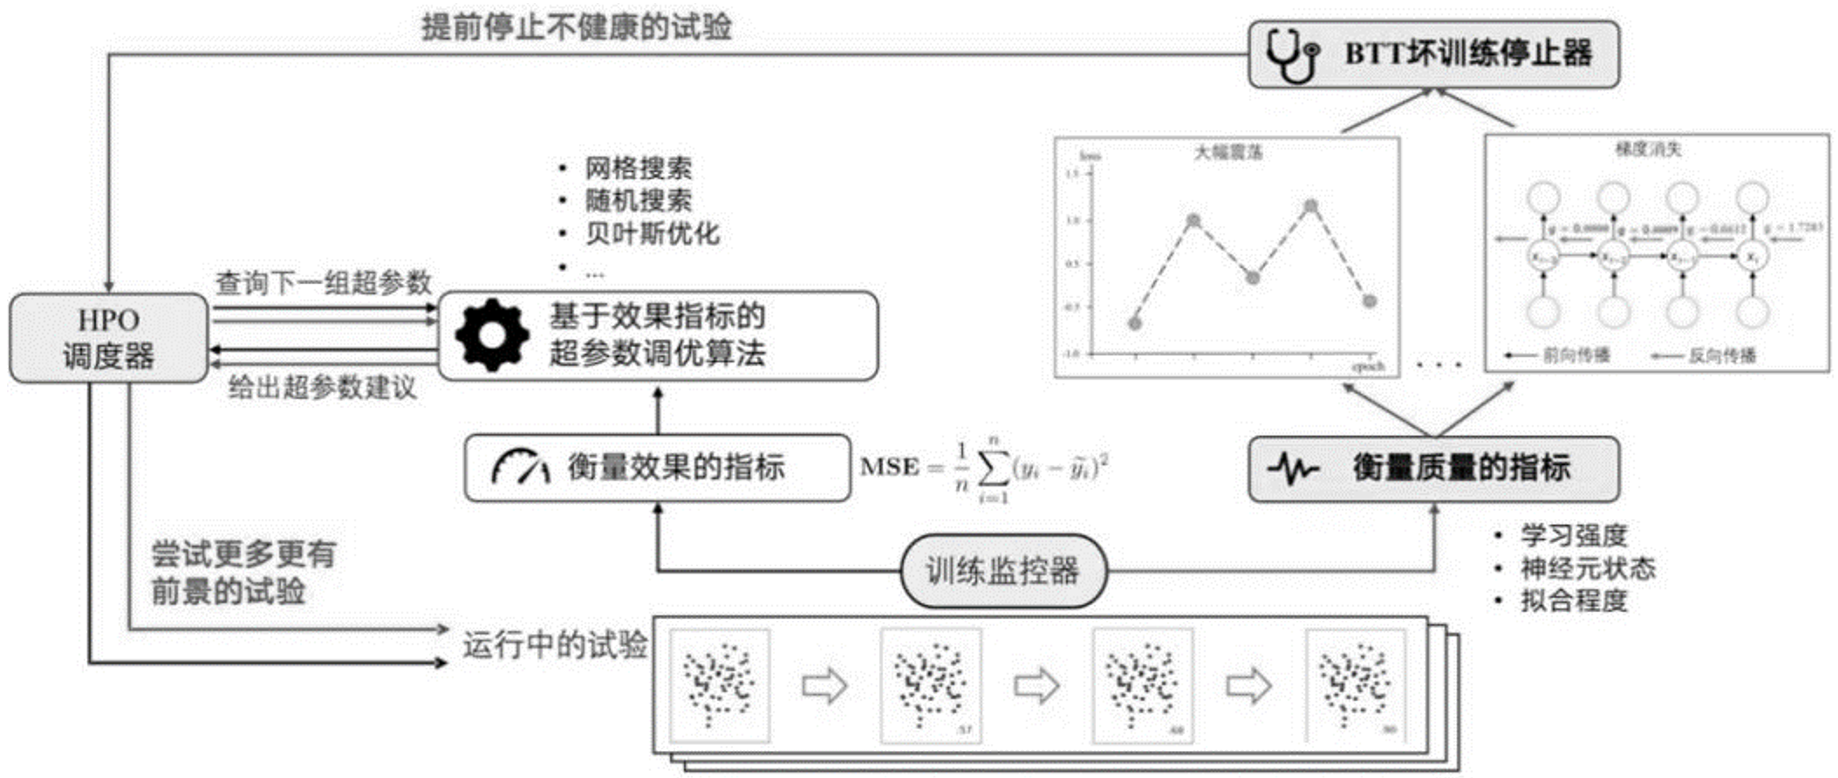
\includegraphics[width=0.8\linewidth]{anytuner-architecture.png}
  \caption{基于训练诊断的超参数调优系统架构}
  \label{fig:anytunerarch}
\end{figure}

(1)指标监测模块:实时监测训练过程中的质量指标,如损失函数值、准确率等。

该模块负责实时监测训练过程中的各种质量指标,如损失函数值、准确率、验证集表现等。
在每个训练迭代中,记录关键指标的变化趋势,并对比历史记录,分析当前超参数组合的性能。
具体实现方式包括在每个训练迭代中,实时记录训练集和验证集的损失函数值和精度,分析其变化趋势。
数据采集通过深度学习框架(如TensorFlow、PyTorch等)的钩子(hook)机制进行,采集训练过程中每个batch的指标数据。
监测内容不仅限于训练集和验证集的损失函数值、训练精度和验证精度,还包括梯度范数、学习率变化等。
具体收集的指标还包括高维度的模型参数值和梯度值的统计量(如中位数、平均值、最大值、方差、四分位数、偏斜值等),以及模型结构信息。
这些指标的收集和分析有助于判断训练过程中的过拟合、欠拟合或训练不稳定等问题。
例如,梯度范数的异常变化可能表明存在梯度爆炸或消失的问题,学习率变化的监控可以帮助识别是否需要调整学习率策略,参数值的统计量则可以揭示模型训练的健康状态。
通过这些措施,能够实时了解和评估每个超参数组合的训练效果,为后续的质量评价和资源调度提供准确的数据支持。

(2)质量评价模块:根据预设的评价标准,对当前超参数组合的训练质量进行评价。

该模块基于预设的评价标准对当前超参数组合的训练质量进行实时评价。
具体实现方式包括采用一系列评价标准,例如提前停止标准、稳定性标准和进展标准。
提前停止标准是指如果在一定的训练迭代内,验证集损失函数未能显著降低,则判定为预期效果不佳。
稳定性标准监测损失函数的波动情况,若波动过大且未能收敛,视为质量不稳定。
进展标准则结合学习率调整策略,评估模型在不同学习率下的表现,判断当前超参数组合的有效性。
评价流程通过设定阈值和规则,自动化地对训练过程中的指标进行分析,生成评价报告。
评价标准设置方面,根据不同任务的需求,设定具体的评价标准和阈值。
例如,损失函数收敛性可以设置为若损失函数在连续若干迭代中下降幅度小于预设阈值,则判定为收敛性不佳;
验证集表现标准则为若验证集损失在一定迭代数内未显著降低,或验证集精度无明显提升,则判定为效果不佳。
通过这些预设的评价标准,模块能够自动化地对每个超参数组合进行评价,生成实时评价报告,从而为后续的资源调度提供依据。

(3)资源调度模块:根据评价结果,提前停止那些预期效果差的超参数组合,并将释放的计算资源重新分配给其他有潜力的超参数组合进行训练。

该模块根据质量评价结果,进行计算资源的智能调度,提前停止那些预期效果差的超参数组合试验,并将释放的计算资源重新分配给其他有潜力的超参数组合进行训练。
具体实现方式包括任务调度器、任务终止器和资源再分配器。
任务调度器负责管理和分配计算资源,根据评价结果动态调整资源分配策略,确保高效利用计算资源。
任务终止器在判定某个超参数组合效果不佳后,及时停止其训练任务,避免资源浪费,并立即释放相应资源。
资源再分配器则将这些释放的资源重新分配给新的超参数组合或正在训练中的有潜力的组合,以加速其训练进程。
调度策略采用优先级调度策略,根据质量评价结果的优先级,灵活调整计算资源的分配,确保资源最大化利用。
通过动态任务调度,系统能够根据质量评价报告实时调整计算资源的分配策略,将资源优先分配给表现良好的超参数组合;
通过提前停止策略,及时终止预期效果差的超参数组合训练任务,避免资源浪费;
通过资源再分配策略,将释放的计算资源高效地重新分配给新的或潜力超参数组合,显著加速其训练过程,从而提高整体调优效率。

\begin{figure}
  \centering
  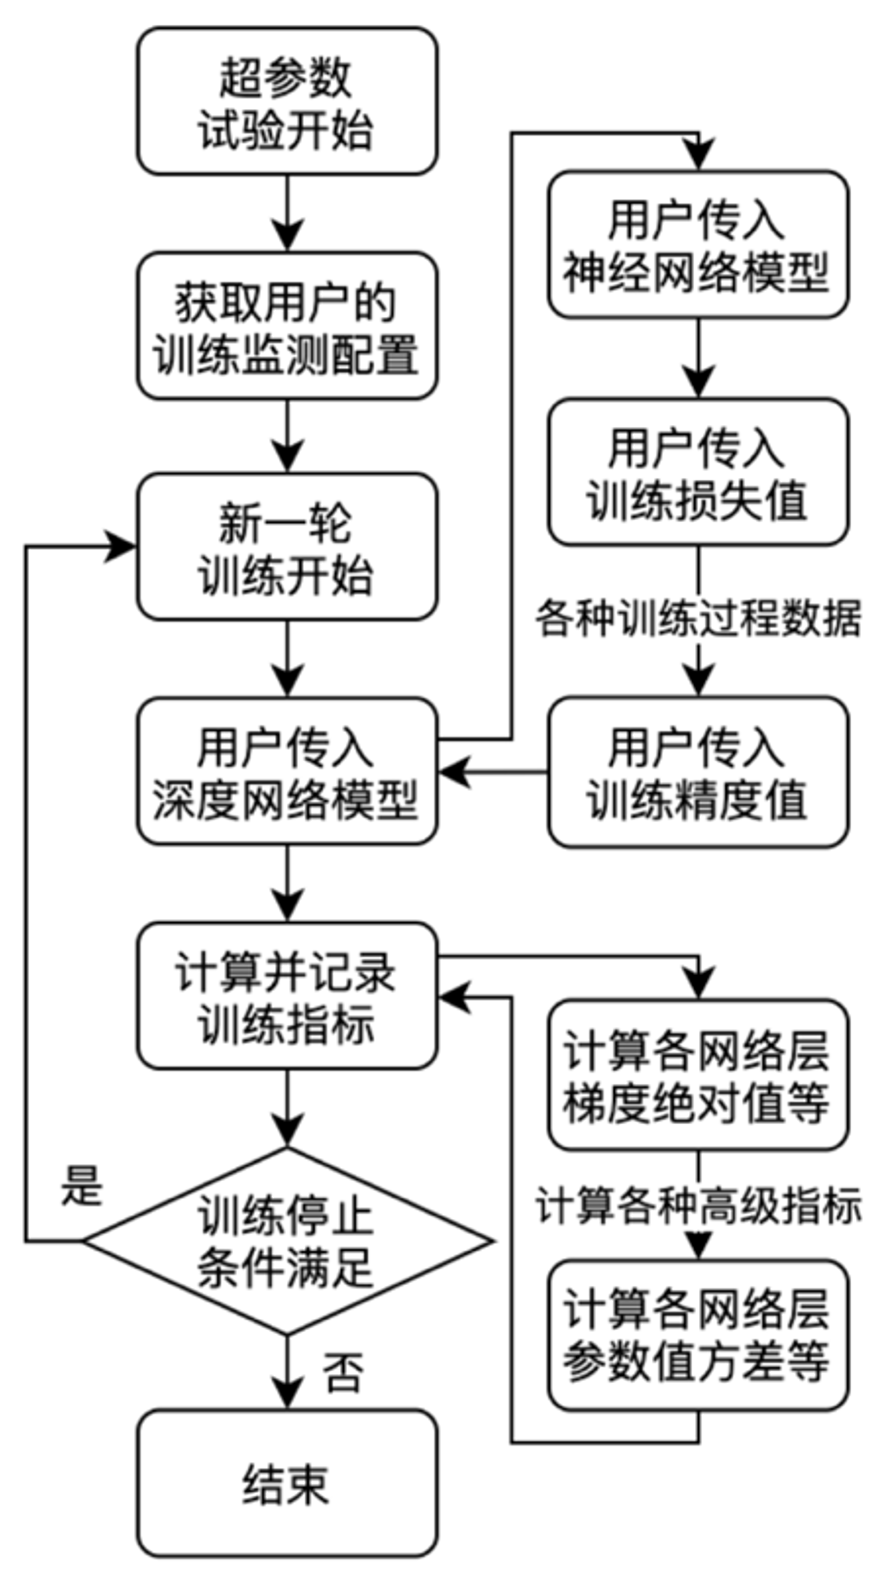
\includegraphics[width=0.3\linewidth]{anytuner-workflow1.png}
  \caption{基于训练诊断的超参数调优工作流程1}
  \label{fig:anytunerworkflow1}
\end{figure}

\begin{figure}
  \centering
  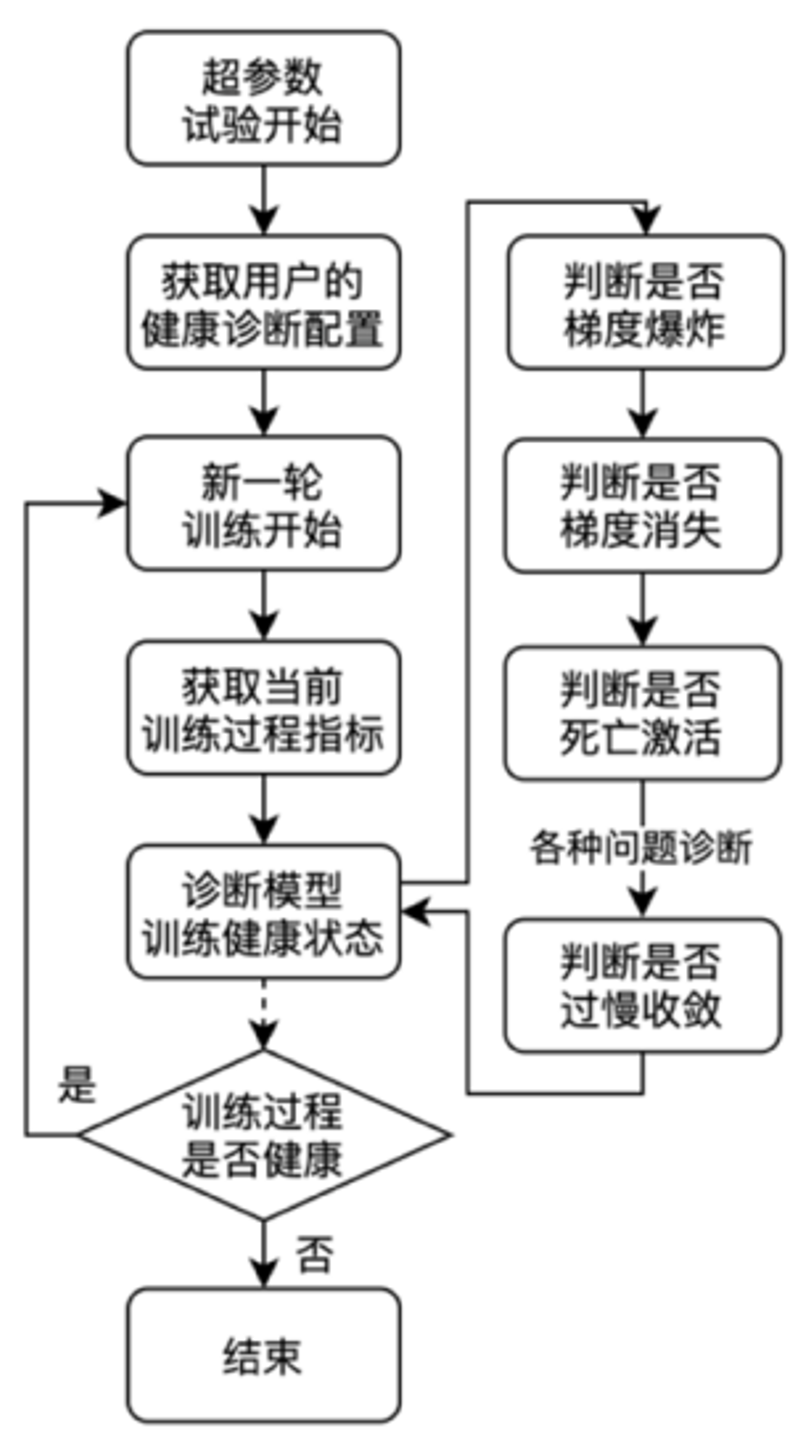
\includegraphics[width=0.3\linewidth]{anytuner-workflow2.png}
  \caption{基于训练诊断的超参数调优工作流程2}
  \label{fig:anytunerworkflow2}
\end{figure}

\begin{figure}
  \centering
  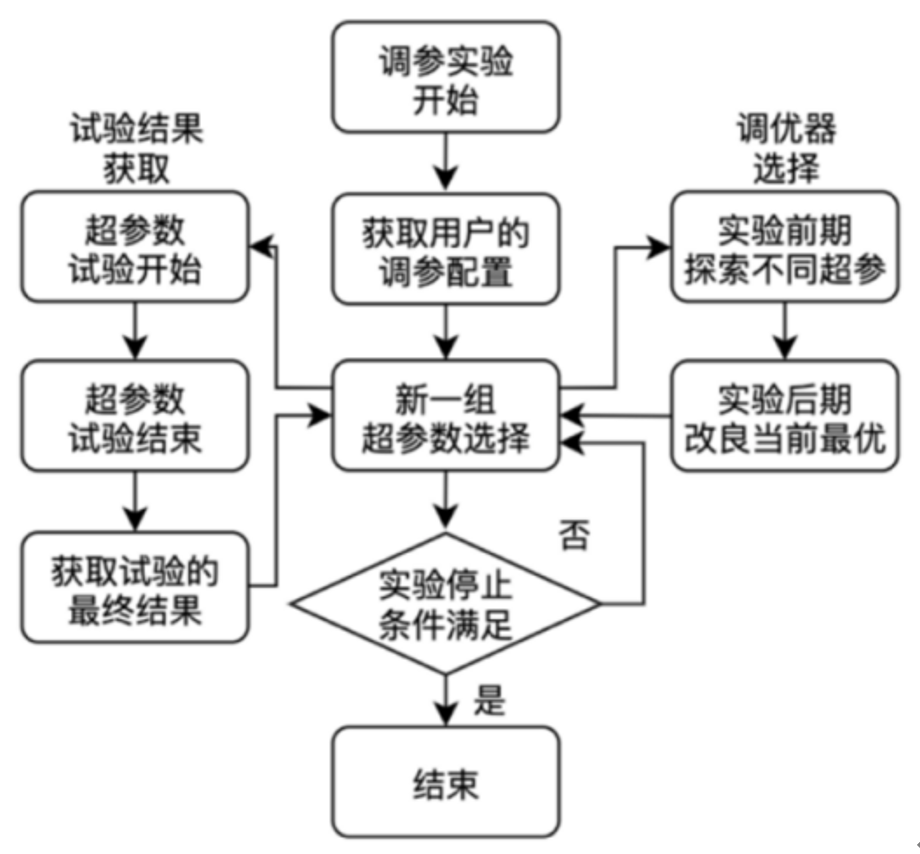
\includegraphics[width=0.5\linewidth]{anytuner-workflow3.png}
  \caption{基于训练诊断的超参数调优工作流程3}
  \label{fig:anytunerworkflow3}
\end{figure}

\subsection{实时质量监测和评价}

实时质量监测:传统的超参数调优方法通常需要等待一个完整的训练周期结束后,才能对超参数组合的效果进行评估。
这种方式的缺点在于,如果一个超参数组合的效果较差,那么只有等待该任务完全结束之后才能重新开始尝试新的组合,导致大量的计算资源浪费。
本技术方案通过实时监测和评价训练过程中的质量指标(如准确率、损失函数值等),可以在训练过程中及时识别和淘汰效果差的超参数组合。
这样,不仅可以减少无效的训练任务,还可以提高调优效率,加快模型的开发速度。

训练质量评价:该技术方案通过一系列预设的评价标准(如提前停止标准、稳定性标准、进展标准等),对当前超参数组合的训练质量进行实时评价。
利用这些评价标准,可以动态地对每个超参数组合的训练效果进行评估,从而在早期阶段就识别出表现不佳的组合,并及时停止这些组合的训练任务。
这种实时的质量评价方式能够有效地减少计算资源的浪费,并提高超参数调优的效率。

\subsection{资源高效利用和动态调度策略}

资源高效利用:在传统的机器学习模型调优过程中,通常会同时运行多个超参数组合的训练任务,以比较它们的效果。
然而,由于每个超参数组合的训练时间可能不同,导致计算资源的利用效率不高。
本技术方案通过提前停止无效训练试验,释放计算资源,并将其用于更有潜力的超参数组合。
具体来说,当一个超参数组合的训练效果已经明显劣于其他组合时,可以提前停止该组合的训练,并将计算资源分配给其他更有潜力的组合。
这样,可以显著提升计算资源的利用效率,加快模型的开发速度。

动态调度策略:传统的机器学习模型调优过程中,通常采用固定的资源分配策略,即每个超参数组合分配相同的计算资源。
这种方式的缺点在于,无法根据超参数组合的训练效果动态调整资源分配,导致资源利用不充分。
本技术方案基于实时评价结果,动态调整训练资源分配策略。
具体来说,当某个超参数组合的训练效果较好时,可以优先分配更多的计算资源给它以及和它相似的其他超参数组合,以加快其训练速度;
反之,当一个超参数组合的训练效果较差时,可以减少其计算资源分配,或者直接提前停止训练,以避免浪费。
通过这种方式,可以确保资源优先分配给预期效果较好的超参数组合,显著提升计算资源的利用效率,提升调优的效果和效率。


\section{大模型微调}

如今,大语言模型已广泛应用在多个领域,其核心能力在于能够根据用户私有数据进行微调,得到用户自有的大模型,以适应特定任务的需求。
本节将介绍大模型微调的技术原理和方法。

\begin{figure}
  \centering
  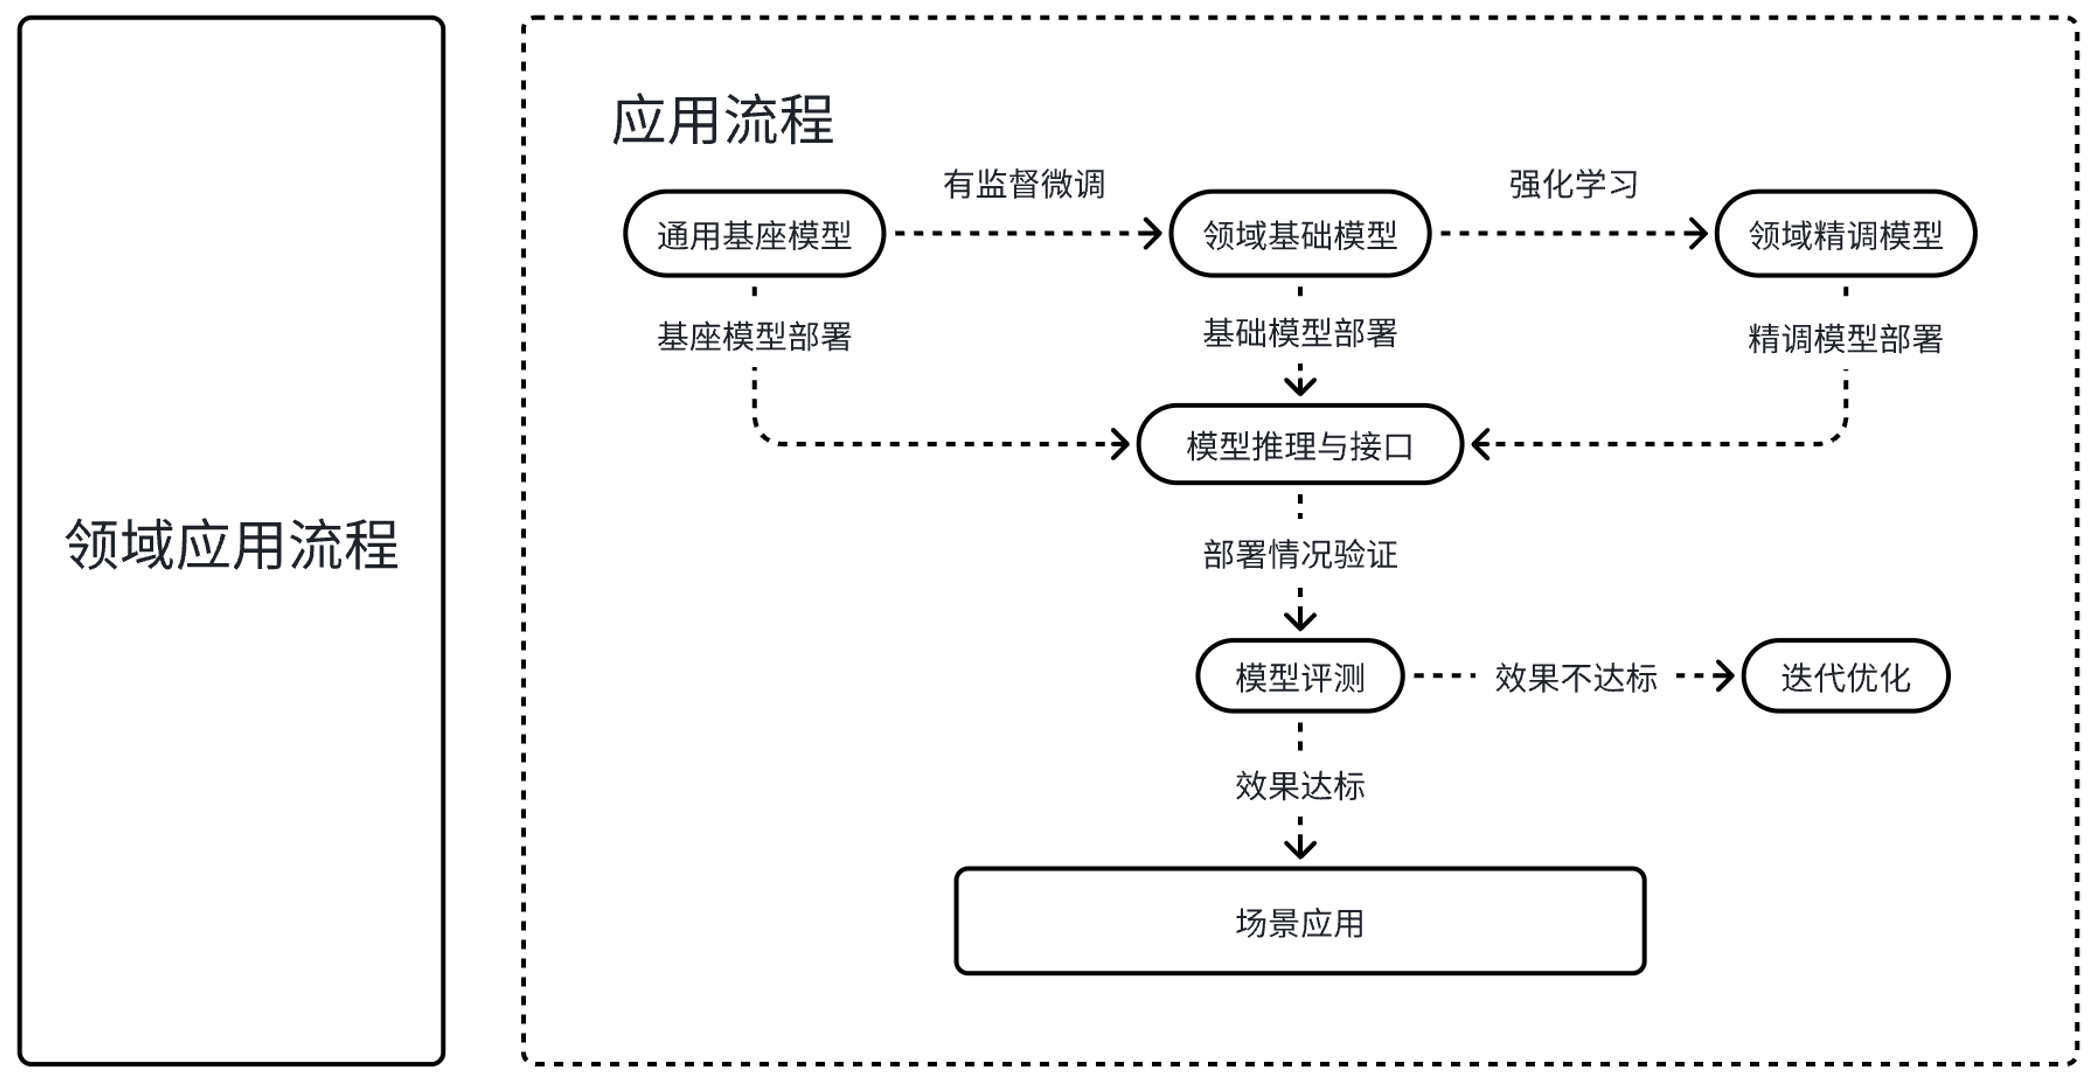
\includegraphics[width=0.8\linewidth]{llm-finetuning-overview.png}
  \caption{大模型微调领域应用流程概览}
  \label{fig:finetuning}
\end{figure}

\subsection{背景问题}

进行大模型微调需要大量的算力与数据作为支撑,是进行大模型微调研究者所需要解决的最基本问题。
微调过程与从头开始训练一个大型深度学习模型同样需要巨大的数据集和计算资源。
这不仅成本高昂,而且对于大多数组织和个人来说,获取和维护这样的资源是不切实际的。
同时,大型模型的参数量巨大,训练它们需要大量的时间和算力与高昂的电力和硬件成本。
另外,为了训练一个表现良好的模型,通常需要大量的标注数据。
在某些领域,获取足够的高质量标注数据是具有挑战性的,特别是对于特定任务或小数据集。

由于微调过程涉及到参数的进一步调整与优化,研究者需要时刻注意预训练任务与微调任务之间的兼容性。
当一个预训练模型在新任务上进行微调时,它可能会忘记之前学到的知识,这限制了模型在新任务上的表现。
尽管大型预训练模型在广泛的任务上表现出色,但它们可能并不完全适应特定的应用领域或特定类型的数据。
大模型微调过程需要尽可能地避免领域不适配带来的模型效果劣化,以最大程度发挥大模型预训练在微调任务上的潜力。

与传统的一次性训练小模型一样,大模型微调要求模型具有定制化的特征。
预训练模型无法覆盖所有应用场景,因此不同的应用场景需要模型针对不同的功能和特性进行定制化微调。
通过微调,可以使模型更好地适应特定领域的需求和特征。
在定制化微调过程中,研究者也希望模型能够保持安全性与泛化性,即在避免危险数据泄露的同时在多种任务上保持出色表现。

\subsection{大模型微调技术原理}

整体步骤上,大模型微调一般分为有监督微调与强化学习两个步骤。
第一,有监督微调使用标注过的数据来调整预训练模型的参数,使其更好地适应特定任务或领域,是较为经典的微调方法。
第二,强化学习模型通过将输入序列分布作为状态空间,将所有可能得token作为动作空间,将特殊设计的奖励模型的输出与策略约束作为价值函数,将大模型下一token选择累计奖励最大化作为策略函数,进一步增强大模型的能力。

微调方式上,大模型可通过全量调整所有参数以充分适应新任务,或采用参数高效微调技术仅优化部分参数以实现快速且低成本的迁移学习。
大模型全量微调随着模型体量的上涨而变得越来越昂贵,促成了参数高效微调技术的广泛探索。

然而,随着针对微调算法的探索不断深入,越来越多的大模型微调算法不断涌现出来。
对于不同的大模型微调任务,不同的算法有着差异化的表现。
如何选择基础模型、如何收集处理领域数据,如何在合适的场景下选择最优的大模型微调方式成为了重要的问题。
为了解决这些问题,我们提出设计一种大模型微调基座平台以加速基础模型、领域数据与微调算法之间的匹配。

\begin{figure}
  \centering
  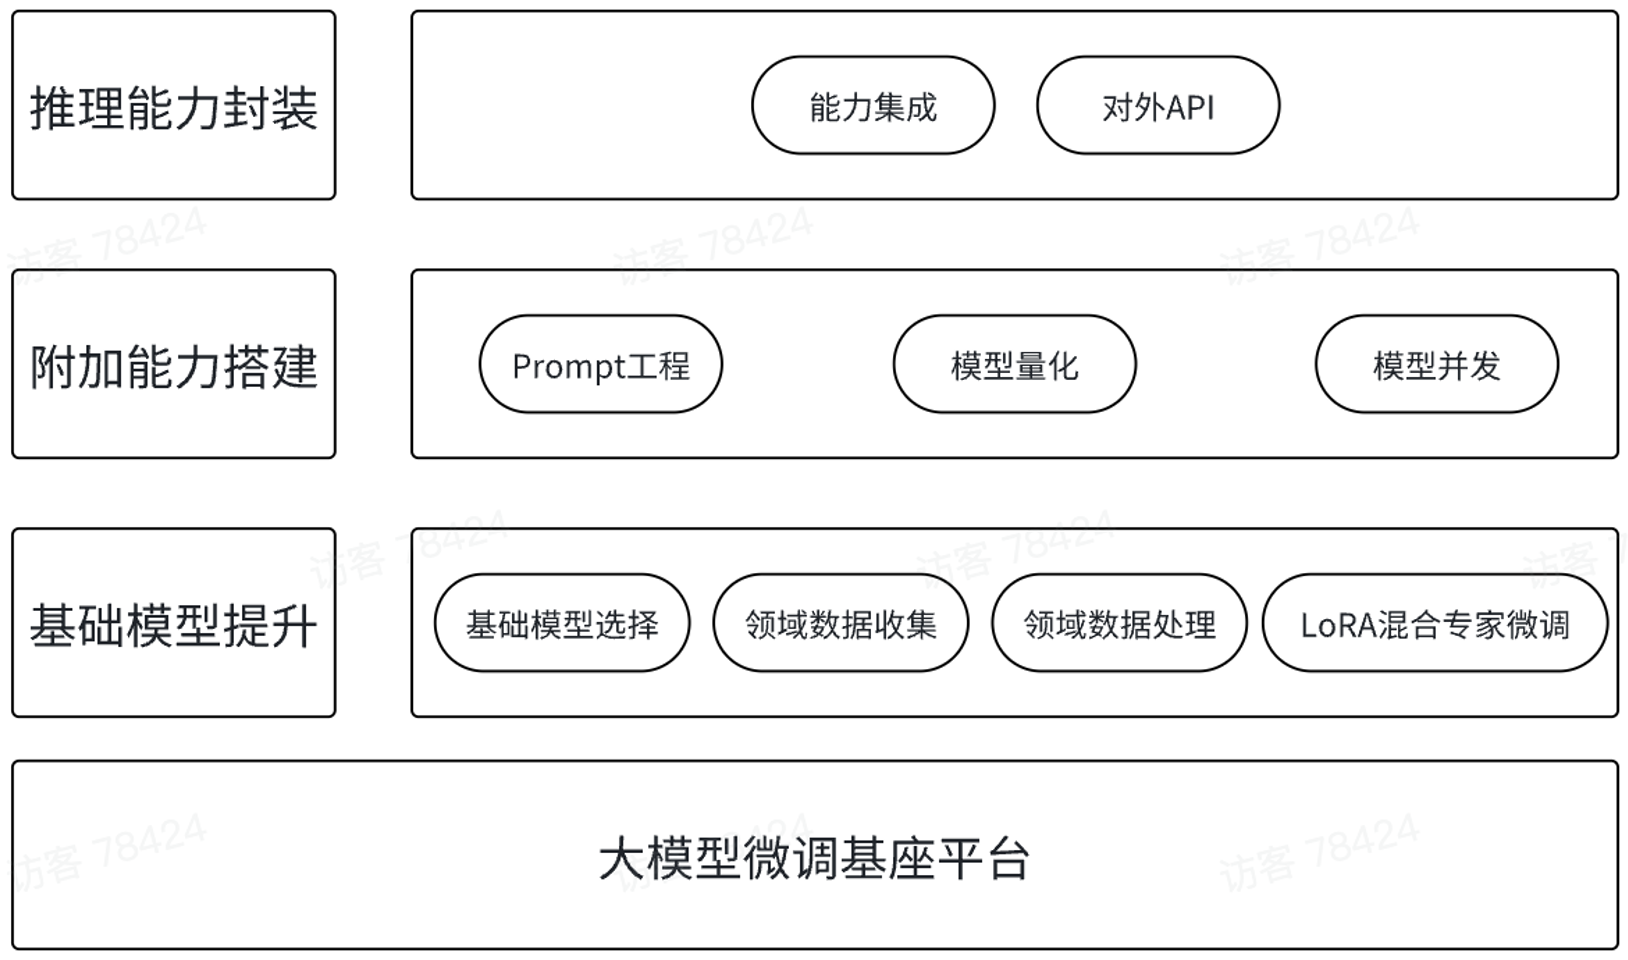
\includegraphics[width=0.8\linewidth]{llm-finetuning-system.png}
  \caption{大模型微调基座平台技术原理}
  \label{fig:finetuningsys}
\end{figure}

大模型微调基座平台包括基础模型提升、附加能力搭建与推理能力封装三部分。
首先,大模型微调基座平台可以通过集成基础模型选择、领域数据收集、领域数据处理与LoRA混合专家微调四个模块来提升基础模型能力。
基础模型选择模块通过在现有的比对指标上进行标准化测试以筛选当前表现较为出色的预训练基础大模型。
领域数据收集模块与领域数据处理模块负责制作用于微调过程的标准化数据,并嵌入任务语义与目标偏好。
最终,通过多种微调方法共同微调的方式使得大模型学习对应的任务语义与目标偏好,实现大模型微调流程。

其次,大模型微调基座平台可以通过Prompt工程、模型量化与模型并发等模块基于基础模型进一步搭建附加能力。
Prompt工程模块弥补了基础模型提升过程中对于目标任务理解偏差的问题,赋予模型通过Prompt理解具体任务需求的能力。
模型量化模块通过低精度浮点数计算进一步压缩了模型微调与推理的计算开销,赋予模型快速微调推理的能力。
模型并发模块通过在流水线、数据与模型权重等维度上的拆分,使得大模型在较小显存的显卡集群上也能有不俗的微调推理表现,赋予模型在低计算资源配置情景下的使用能力。

最终,大模型基座平台可以通过能力集成与对外API模块实现云端的快速部署。
能力集成模块基于面向对象编程思想,将平台的全部功能进行必要的合并与拆分,形成针对大模型微调场景的函数工具箱。
对外API模块将基座平台的主要功能以REST API等形式进行封装,主要负责基座平台对用户提供的云服务。

\subsection{混合专家系统}

混合专家系统(Mixture of Experts, MoE)是在神经网络领域发展起来的一种集成学习(Ensemble Learning)技术。
传统的深度学习模型在训练时,对于每个输入样本,整个网络都会参与计算。
随着模型越来越大,训练使用的样本数据越来越多,训练的开销越来越难以承受。
而MoE可以动态激活部分神经网络,从而实现在不增加计算量的前提下大幅度增加模型参数量。

MoE 技术目前是训练万亿参数量级模型的关键技术。
MoE 将预测建模任务分解为若干子任务,在每个子任务上训练一个专家模型(Expert Model),开发一个门控模型(Gating Model),该模型根据要预测的输入来学习信任哪个专家,并组合预测结果。尽管该技术最初是使用神经网络专家和门控模型来描述的,但它可以推广到使用任何类型的模型。

\subsection{LoRA}

LoRA(Low-Rank Adaptation)是一种旨在微调大型预训练语言模型(如GPT-3或BERT)的技术。
其核心理念在于,在模型的决定性层次中引入小型、低秩的矩阵来实现模型行为的微调,而无需对整个模型结构进行大幅度修改。
这种方法的优势在于,在不显著增加额外计算负担的前提下,能够有效地微调模型,同时保留模型原有的性能水准。

由于LoRA的出色性能,部分工作尝试对LoRA进行升级改进。
QLoRA(Quantized Low-Rank Adaptation)是一种结合了LoRA(Low-Rank Adaptation)方法与深度量化技术的高效模型微调手段。
这种方法采用创新的技术将预训练模型量化为4位,包括低精度存储数据类型(4-bit NormalFloat,简称NF4)和计算数据类型(16-bit BrainFloat),极大地减少了模型存储需求,同时保持了模型精度的最小损失。

与LoRA技术类似,适配器调整(Adapter Tuning)的目标是在保留预训练模型原始参数不变的前提下,使模型能够适应新的任务。
适配器调整的方法是在模型的每个层或选定层之间插入小型神经网络模块,称为“适配器”。
这些适配器是可训练的,而原始模型的参数则保持不变。

LoRA混合专家微调同样遵循混合专家模型的一般流程。用于训练多个模型以解决复杂任务的技术。
大模型微调基座平台会针对不同的任务和数据,选择特定数量的LoRA来充当专家模型。具体流程如下:

(1)准备搜集数据:
收集和准备用于训练的数据集。数据集应该包含输入特征和对应的目标值(或标签),以及特定LoRA标识。
需要知道哪个任务应该由哪个专家模型处理。

(2)选择专家(LoRA)数量:
决定使用多少个专家模型。
这通常根据任务的复杂性和数据集的规模来选择。
专家数量可以根据经验进行调整,也可以通过交叉验证等方法选择。

(3)初始化专家(LoRA)模型:
初始化每个专家模型的参数。
可以使用随机初始化或者预训练模型来初始化。
这边的LoRA是随机初始化的。

(4)训练专家(LoRA)模型:
根据特定任务为每个LoRA模型分别训练参数。
这通常是标准的模型训练过程,使用输入特征和对应的目标值来更新模型参数。
可以使用梯度下降等优化算法进行参数更新。

(5)训练门控模型(Gating):
门控模型的标签实际上是每个输入对应的专家模型的标识。
门控模型通过学习输入特征与对应的专家模型之间的关系,来决定选择哪个专家模型来处理输入。
训练过程的目标是最小化分类误差,使门控模型能够准确地选择适当的专家模型。

(6)前向传播和损失计算:
将输入特征通过专家模型和门控模型进行前向传播,得到每个专家模型的预测结果和门控模型的预测结果。
然后,计算损失函数,该损失函数包括专家模型的损失和门控模型的损失。

(7)反向传播和参数更新:
使用反向传播算法计算整个Mixture of LoRA模型的梯度,并更新所有模型的参数,包括专家模型和门控模型。

(8)迭代训练:
重复训练过程,多次迭代更新参数,直到模型收敛或达到预定的训练迭代次数。

(9)评估和调优:
使用验证集或测试集来评估模型性能,根据性能表现进行调优,可以调整专家数量、门控模型的结构、训练参数等。


\section{模型更新}

模型开发完成后,集成进入业务系统生产环境,持续接入真实业务数据并进行推理。
然而,真实数据与训练数据之间客观存在的分布差异会导致模型效果随时间推移而下降,需要及时更新模型以保持模型的性能。
本节就模型更新的相关技术进行介绍。

\subsection{背景问题}

机器学习模型的一种常见的开发和应用流程大致是,开发者首先面向目标场景设计出一套机器学习算法或是直接选用现成算法,接着准备一定量的能够代表目标场景的数据(即训练集),然后用准备好的算法在准备好的训练集的基础上训练出表现良好的模型,最后再把训练好的模型部署到生产环境。
根据机器学习的理论,在线下表现良好的模型在线上也能表现良好的一个前提是,模型在线上所接触到的数据与用来训练该模型的数据服从相同的统计分布,而这个前提在现实中却经常会被打破。
在现实场景中,各种各样的因素都会带来线上数据分布随时间变化进而偏离训练集数据分布的结果,业界把这种线上数据分布随时间变化的现象称为数据偏移。

应对数据偏移问题的一种直接的思路是,首先通过某种方法来检测潜在的数据偏移(即偏移检测),在检测到数据偏移后再通过某种方法来更新模型以让模型适应新的数据分布(即偏移适配)。
大多数偏移检测方法监视模型预测效果随时间的变化,在模型效果的下降具有统计显著性时汇报偏移,我们把这类方法称为基于模型效果的偏移检测方法;
除此之外,也有一些偏移检测方法选择直接监视输入数据分布随时间的变化,我们把这类方法称为基于输入分布的偏移检测方法,这类方法相比基于模型效果的偏移检测方法的优点在于不需要线上数据的真实标签就能够工作(评价模型预测效果需要真实标签),但也存在计算成本过高和敏感度过高等问题。
至于偏移适配,最通用的偏移适配方法是用属于新分布的数据来训练新模型取代旧模型;
除此之外,也有一些模型相关的偏移适配方法被提出。
除了先做偏移检测再做偏移适配,还有一种思路是直接做偏移适配,这类偏移适配方法包括一些基于集成学习的方法,它们隐含了感知数据偏移的能力,会依据新到来的数据持续更新模型,不需要与专门的偏移检测方法配合使用。
为方便后面叙述,我们把包括上述方法在内的为解决数据偏移问题而提出的方法统称为偏移对策。

尽管目前已经有很多种偏移对策,但对不熟悉数据偏移领域的研发人员来说,把这些对策应用于实际场景仍然存在困难。

不同的对策和这些对策的不同参数取值(以下合称对策)所适用的数据偏移场景(如渐替偏移的渐替速率、是否存在概念重现)是不同的。
为了给目标场景选取合适的对策,研发人员不但需要对多种对策以及它们的工作机制有所了解,还需要对目标场景的数据偏移特性有所认识,这就给研发人员带来了使用门槛。

即使研发人员有能力为目标场景选取合适的对策,也还面临在生产环境中合理使用所选对策的难题。
生产环境中往往存在一些复杂的情况,例如输入数据的真实标签可能延迟到来、乱序到来甚至缺失,或是模型更新期间可能仍有新的输入数据到来,等等。
为此,研发人员需要为模型和偏移对策设计和实现合理的实际运行逻辑。
这里的难点有两个,一是研发人员需要周全考虑生产环境中的各种可能情况以免造成意外后果,二是合理的实际运行逻辑将涉及历史数据的暂存和异步维护,这要求研发人员具有一定的多线程编程能力。

即使研发人员有能力为模型和偏移对策设计和实现合理的实际运行逻辑,也还面临在部署之前评测所选偏移对策的难题。
评测本质上是对实际运行过程的模拟,其难点在于确保逻辑与实际运行等价的同时尽可能地节省时间。
目前也有一些现成的偏移对策评价方法,但这些方法并不满足逻辑与实际运行等价的条件(因为它们并非是针对某种模型和偏移对策实际运行逻辑开发出来的),而且往往对生产环境的情况做了较大的简化,因此这些方法所给出的评价结果不一定能符合生产环境的情况。

\subsection{模型更新策略评价}

为降低研发人员把现有偏移对策应用于实际场景的门槛,本技术将帮助研发人员构造具有数据偏移自适应能力的模型服务。

技术主要流程如下图所示,分构造和运行两个阶段。
在构造阶段,研发人员首先以“手动”或“自动”的方式构造模型更新策略,即偏移检测器和模型更新器(如重新训练和微调)的结合,然后再基于所构造出来的模型更新策略构造模型服务。
在运行阶段,模型服务接收输入数据并返回模型预测值,同时接收真实标签,并持续检测潜在的数据偏移,在检测到数据偏移时更新模型。
在构造阶段,如果研发人员自己有一些选取偏移对策的思路,则可以通过给定偏移检测器和模型更新器来手动构造模型更新策略并使用本技术的模型更新策略评测功能,根据评测结果来调整模型更新策略所使用的偏移检测器和模型更新器的配置,最终得到合适的模型更新策略用于模型服务构造;
如果研发人员不熟悉数据偏移领域,则无须给定偏移检测器即可使用本技术的模型更新策略自动构造功能来自动构造出合适的模型更新策略。

为降低研发人员把现有偏移对策应用于实际场景的门槛,本技术将帮助研发人员构造具有数据偏移自适应能力的模型服务。

技术主要流程如图\ref{fig:modelupdate}所示,分构造和运行两个阶段。
在构造阶段,研发人员首先以“手动”或“自动”的方式构造模型更新策略,即偏移检测器和模型更新器(如重新训练和微调)的结合,然后再基于所构造出来的模型更新策略构造模型服务。
在运行阶段,模型服务接收输入数据并返回模型预测值,同时接收真实标签,并持续检测潜在的数据偏移,在检测到数据偏移时更新模型。
在构造阶段,如果研发人员自己有一些选取偏移对策的思路,则可以通过给定偏移检测器和模型更新器来手动构造模型更新策略并使用本技术的模型更新策略评测功能,根据评测结果来调整模型更新策略所使用的偏移检测器和模型更新器的配置,最终得到合适的模型更新策略用于模型服务构造;
如果研发人员不熟悉数据偏移领域,则无须给定偏移检测器即可使用本技术的模型更新策略自动构造功能来自动构造出合适的模型更新策略。

\begin{figure}
  \centering
  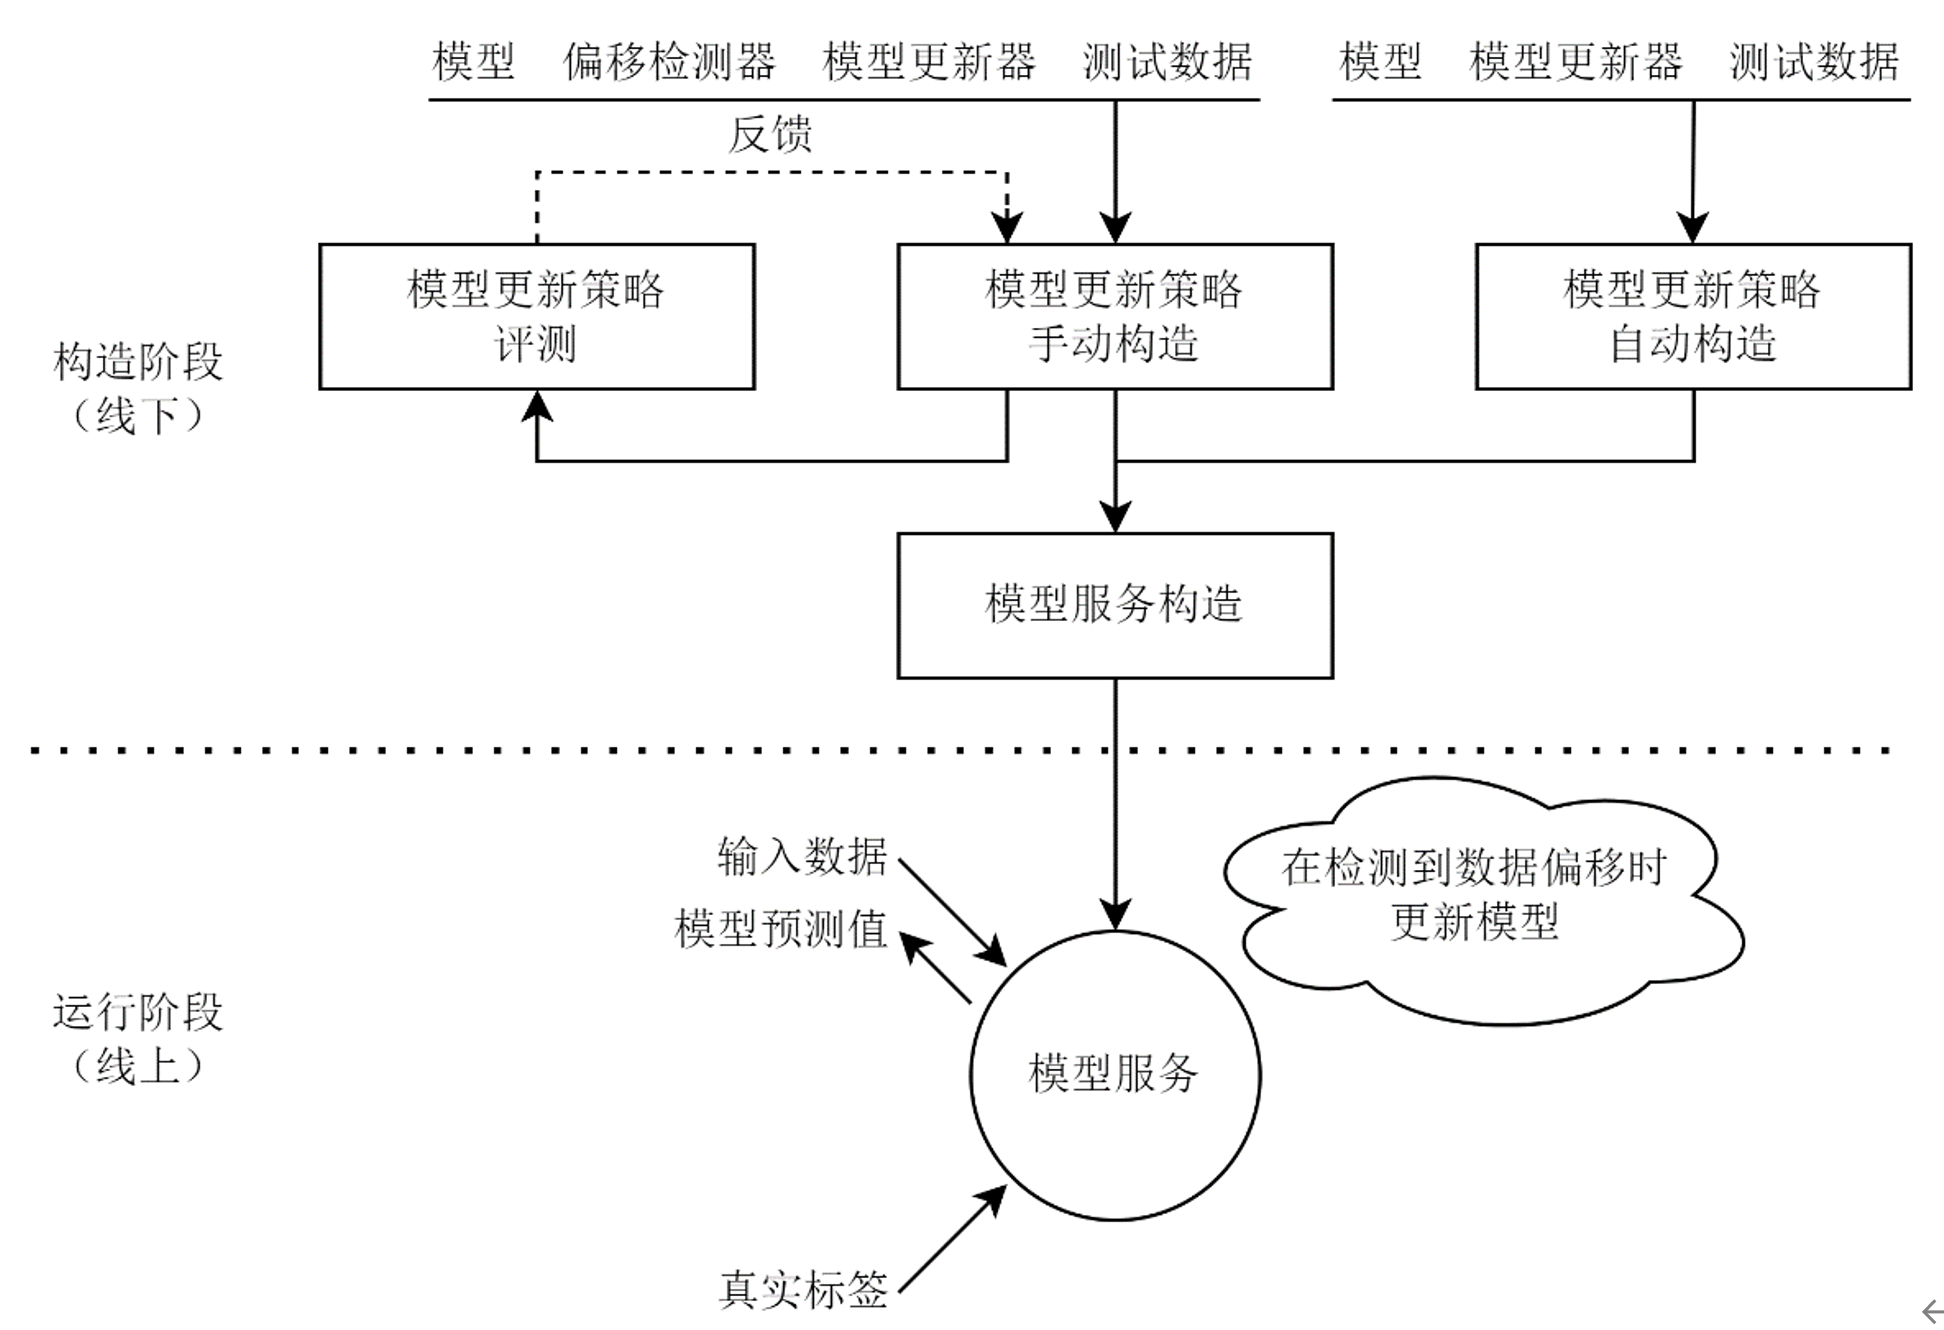
\includegraphics[width=0.8\linewidth]{model-update.png}
  \caption{模型更新策略评测与推荐流程}
  \label{fig:modelupdate}
\end{figure}

\subsection{模型服务构造}

本技术需要设计和实现一套模型服务中模型和模型更新策略的实际运行逻辑,其负责线上数据的接收和处理并成为模型服务的一部分。

在偏移检测器汇报数据偏移后,模型更新需要最近若干条样本的输入值和真实标签,模型服务内部需要一个“暂存区”来暂存已经接收到的输入值和真实标签。
考虑到基于模型效果的偏移检测器在工作时需要样本的真实标签和模型预测值来计算样本预测效果指标值,而真实标签的到来通常是有延迟的,模型服务需要把模型预测值也暂存下来。
为了让偏移检测和模型更新的过程与模型预测的过程互不干扰,除暂存区外,模型服务还需要一个独立的“偏移检测线程”来把暂存下来的数据发送给偏移检测器并在偏移检测器汇报数据偏移后执行模型更新。

\subsection{模型更新策略评测}

针对模型服务中模型和模型更新策略的实际运行逻辑,本技术需要设计和实现相应的模型更新策略评测功能。
研发人员给定模型、模型更新策略和带时间戳的测试数据,即可通过评测来模拟模型服务在实际运行时的情况并获得模型全局评价指标等与模型更新策略好坏有关的信息。

为实现符合生产环境实际情况的精确评测,本技术的评测方法将依据研发人员所给定的带时间戳的测试数据来一步步地执行模型服务偏移检测线程的步骤,同时推算其实际运行过程中每一步的完成时刻,进而在模型服务各个时刻状态的基础上推算出每个样本的预测值,最后得到模型全局平均预测效果指标。

为实现评测逻辑与模型服务实际运行逻辑的解耦,本技术还将提出一种把模型服务视为黑盒的评测方法,该方法将按照时间间隔来把各条数据发送给模型服务,同时一旦发现模型服务进入等待下一条数据的空闲状态,就立即发送下一条数据。
为检测模型服务的空闲状态,该评测方法将要求模型服务维护一个“活跃计数”,该计数的大致含义是“当前相关活跃线程的数量上界”。
这样一来,只须检测活跃计数下降到零的事件,就能检测模型服务的饥饿状态。

\subsection{模型更新策略自动构造}

在模型更新策略评测功能的基础上,本技术需要设计和实现模型更新策略的自动构造功能。
研发人员给定模型、模型更新器和带时间戳的测试数据,即可由该功能自动选择合适的偏移检测算法和参数取值(还可以包括模型更新器的参数取值,如微调学习率和迭代次数),进而形成构造模型服务所需的模型更新策略。

模型更新策略自动构造本质上是对偏移检测器和模型更新器的超参数优化。
考虑到影响模型更新策略优劣的因素不但包括模型预测效果指标还包括模型更新的计算成本代价,本技术需要实现模型更新策略的多目标优化;
针对偏移检测器的超参数优化,为降低研发人员的使用门槛,本技术需要定义一套合理的默认搜索空间以达到无须研发人员手动指定的效果;
为充分利用计算资源,本技术需要设计和实现一套易于研发人员使用的多CPU核心和多GPU并行搜索机制。

\begin{figure}
  \centering
  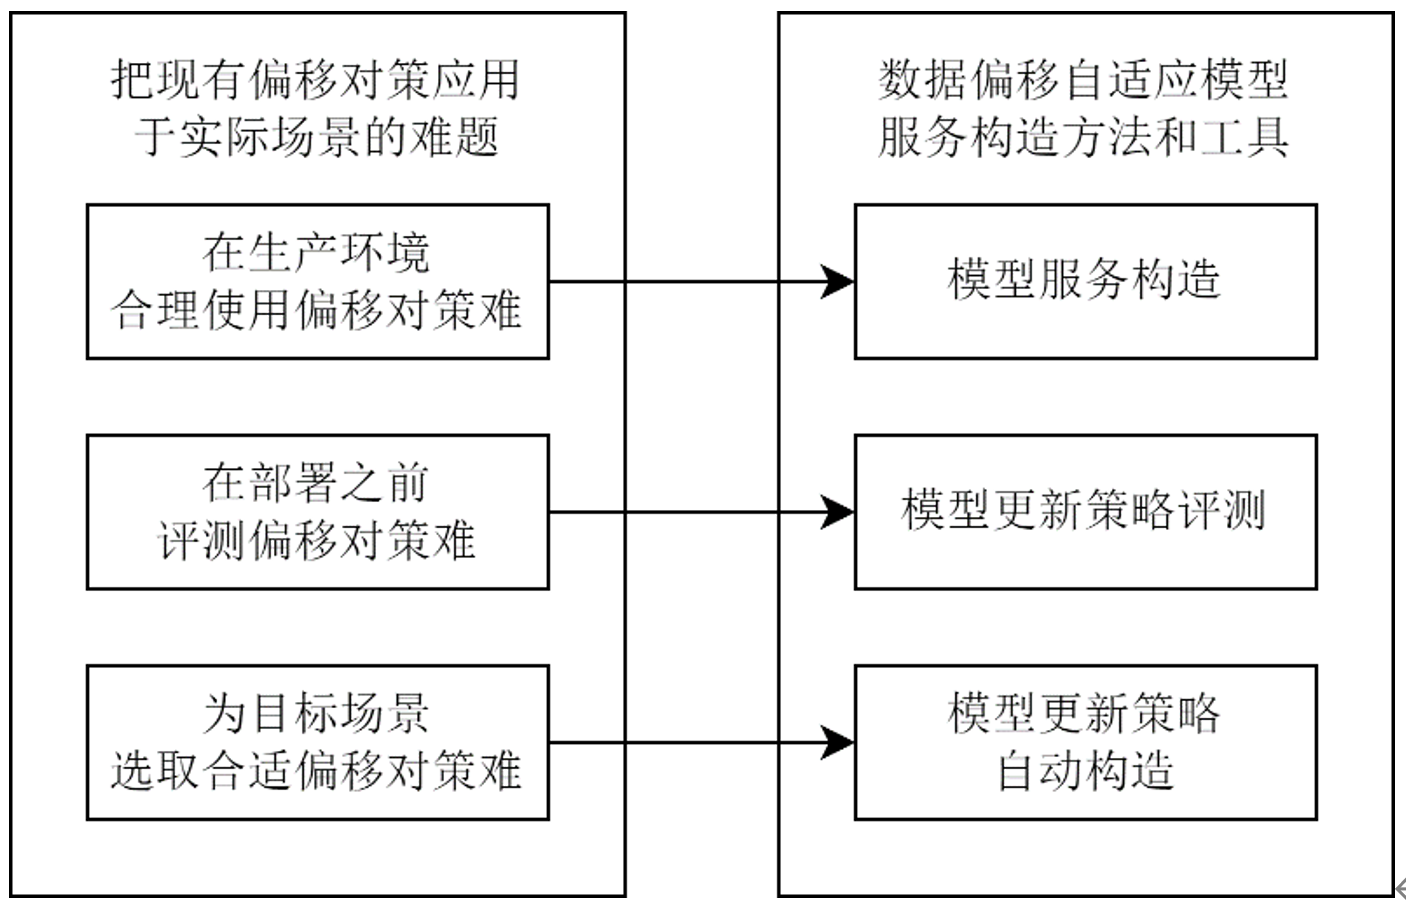
\includegraphics[width=0.5\linewidth]{model-update-auto.png}
  \caption{模型更新策略自动构造}
  \label{fig:automodelupdate}
\end{figure}

% !TeX root = ../thuthesis-example.tex

\chapter{系统实现:大数据机器学习研发管理系统Anylearn}

Anylearn是一款大数据机器学习研发管理系统,支持数据集、算法族、模型库等资产管理,支持机器学习研发过程管理、知识沉淀、模型迁移,满足团队资源统筹利用、团队高效协作等人工智能工程化需求。

2017年,大数据系统软件国家工程研究中心(原大数据系统软件国家工程实验室)成立,旨在推动大数据系统软件领域的科研和产业发展。
依托大数据系统软件国家工程研究中心资源和平台,软件学院机器学习组开始快速拓展人工智能相关研究和应用落地。
在此过程中,如何有效地对机器学习模型研发进行管理、提高模型落地应用效率成为了一个重要问题。
Anylearn作为机器学习平台应运而生。

在项目初期,团队对Anylearn的主要需求在于系统化地打通数据到模型的稳定通路,并高效地管理团队的GPU资源,避免资源争抢和浪费,提高资源使用效率。
在后续发展过程中,团队逐渐意识到机器学习科学研究中更关注的是研发迭代的功能支持和管理手段。
Anylearn通过多年的发展,支持了面向算法开发者的SDK、自定义算法上传、多样化的训练环境、训练过程跟踪、超参数调优、训练结果预览等偏向模型训练的功能,以及面向各类用户管理需求的用户首页、主管页面、管理员页面等功能。
目前,Anylearn在机器学习研发过程管理和资产管理方面也逐渐形成体系,围绕训练任务建立起过程记录和资产关联,支持团队的知识沉淀和协作。

\section{使用场景}

为了便于介绍Anylearn的使用场景和典型工作流程,将Anylearn从概念上分为以下部分:
\begin{itemize}
  \item Anylearn云环境,即Anylearn长活系统线上环境(https://anylearn.nelbds.cn/);
  \item Anylearn交互网页,即Anylearn云环境的Web页面;
  \item Anylearn客户端SDK(https://pypi.org/project/anylearn/)。
\end{itemize}

Anylearn交互网页的主要模块包括:训练项目、数据集、算法族、模型库、镜像中心、计算资源概况以及用户中心等。

\subsection{场景一:将本地机器学习项目适配至Anylearn云环境}

用户在本地(PC、开发服务器等自有环境)已开展机器学习项目的研发,已经明确了要使用的数据集、算法、预训练模型。算法经调试,已成功在本地运行了小规模训练。
用户希望将此机器学习项目适配到Anylearn云环境,使用更多算力和研发管理功能进行更大规模的训练和验证。

具体步骤如图\ref{fig:scenario1}所示。

\begin{figure}
  \centering
  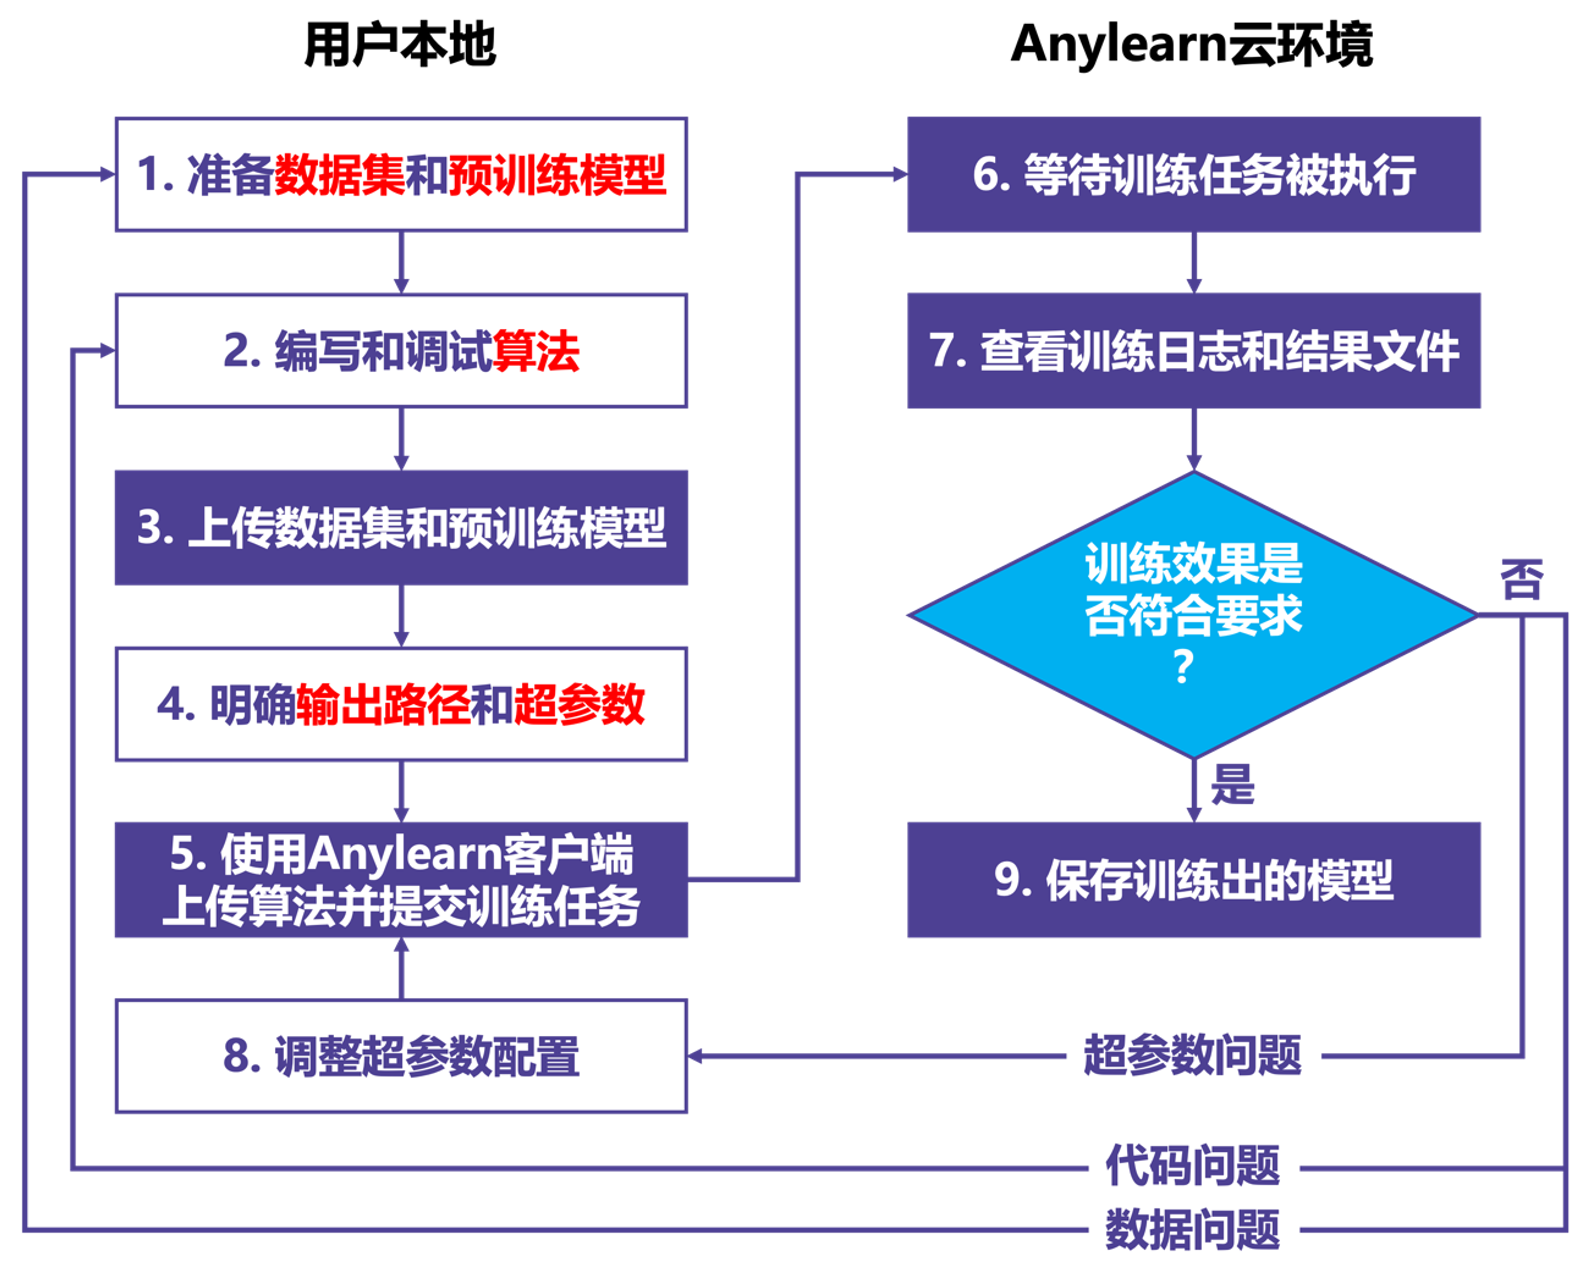
\includegraphics[width=0.8\linewidth]{anylearn-scenario1.png}
  \caption{Anylearn使用场景一:本地项目适配至云环境}
  \label{fig:scenario1}
\end{figure}

(1)用户根据机器学习项目需求,在本地已准备好数据集和预训练模型。
根据机器学习任务的不同,可能会使用一个或多个数据集和预训练模型(例如:域适应迁移学习),也可能不需要数据集和模型。

(2)用户在本地已编写并调试好机器学习算法,已在本地使用上述数据集和预训练模型初步跑通训练和验证。

(3)用户前往Anylearn交互网页并注册账户。
然后,用户通过Anylearn交互网页将步骤1中的数据集和预训练模型分别上传至Anylearn云环境。
当数据集或预训练模型的规模较大时(依据经验,超过500MB即为大),通过Anylearn交互网页上传效率较低,应当联系Anylearn系统管理员通过其他方式上传。
需要注意的是,由于网络条件有限,在Anylearn云环境中执行训练时从外网下载数据集和模型通常非常缓慢,使用torchvision、huggingface等库进行自动下载的数据集和模型需要提前上传到Anylearn云环境。

(4)用户需梳理并明确机器学习算法的输出路径和超参数。
输出可能包括:模型检查点文件(checkpoints)、最终模型参数文件(weights)、TensorBoard日志文件、模型验证效果文件等等。
Anylearn云环境中要求这些输出均需要写入到一个统一的路径下,该路径应当是以算法目录下的一个子目录(例如:假设用户本地的算法存放在/workspace/myuser/myalgo下,本步骤中涉及的输出可以写入./results目录,即绝对路径/workspace/myuser/myalgo/results,但不可写入算法目录以外的/data/results路径下)。

(5)用户在本地安装Anylearn客户端SDK。
用户可能需要修改步骤(2)中的本地算法代码。
用户在本地编写一个Python脚本,调用Anylearn客户端库(SDK),将本地算法上传至Anylearn云环境,并向Anylearn云环境提交一个训练任务。

(6)用户前往Anylearn交互网页,查看上述提交的训练任务的状态。
由于计算资源有限,提交的训练任务可能无法马上执行,需排队等待资源释放。

(7)当训练任务开始执行后,用户在Anylearn交互网页中查看训练任务的日志、系统监控等信息,判断训练执行情况以及训练出的模型的效果。

(8)当用户发现训练有问题时:
\begin{enumerate}
  \item 当训练超参数存在问题时,用户在本地算法或步骤5中编写的本地Python脚本中修改超参数配置,重新执行本地Python脚本以上传修改后的算法并提交一个新的训练任务,即重复步骤(5)及其后续步骤;
  \item 当训练代码(例如:数据加载方式、模型架构、优化器使用等等)存在问题时,用户调整本地算法代码,上传修改后的算法并提交一个新的训练任务,即重复步骤(2)及其后续步骤;
  \item 当数据集存在问题时,用户调整数据集或重新准备数据集,并将修改后的数据集当做一个新的数据集上传至Anylearn云环境(已存在的数据集不支持变更文件),即重复步骤(1)及其后续步骤。
\end{enumerate}

(9)当用户认为训练出的模型达到预期效果时,用户在Anylearn交互网页上将训练出的模型参数文件转存至Anylearn云环境的模型库,形成模型资产。

\subsection{场景二:参与Anylearn云环境上已存在的机器学习项目}

机器学习项目组已在Anylearn上开展工作,用户作为新进组的成员,对已经在Anylearn云环境中跑通的算法进行迭代优化。
用户需将项目组先前上传至Anylearn云环境的数据集、预训练模型和算法下载至本地(PC、开发服务器等自有环境),对算法进行调整,再将算法上传回Anylearn云环境并进行训练和验证。

具体步骤如图\ref{fig:scenario2}所示。

\begin{figure}
  \centering
  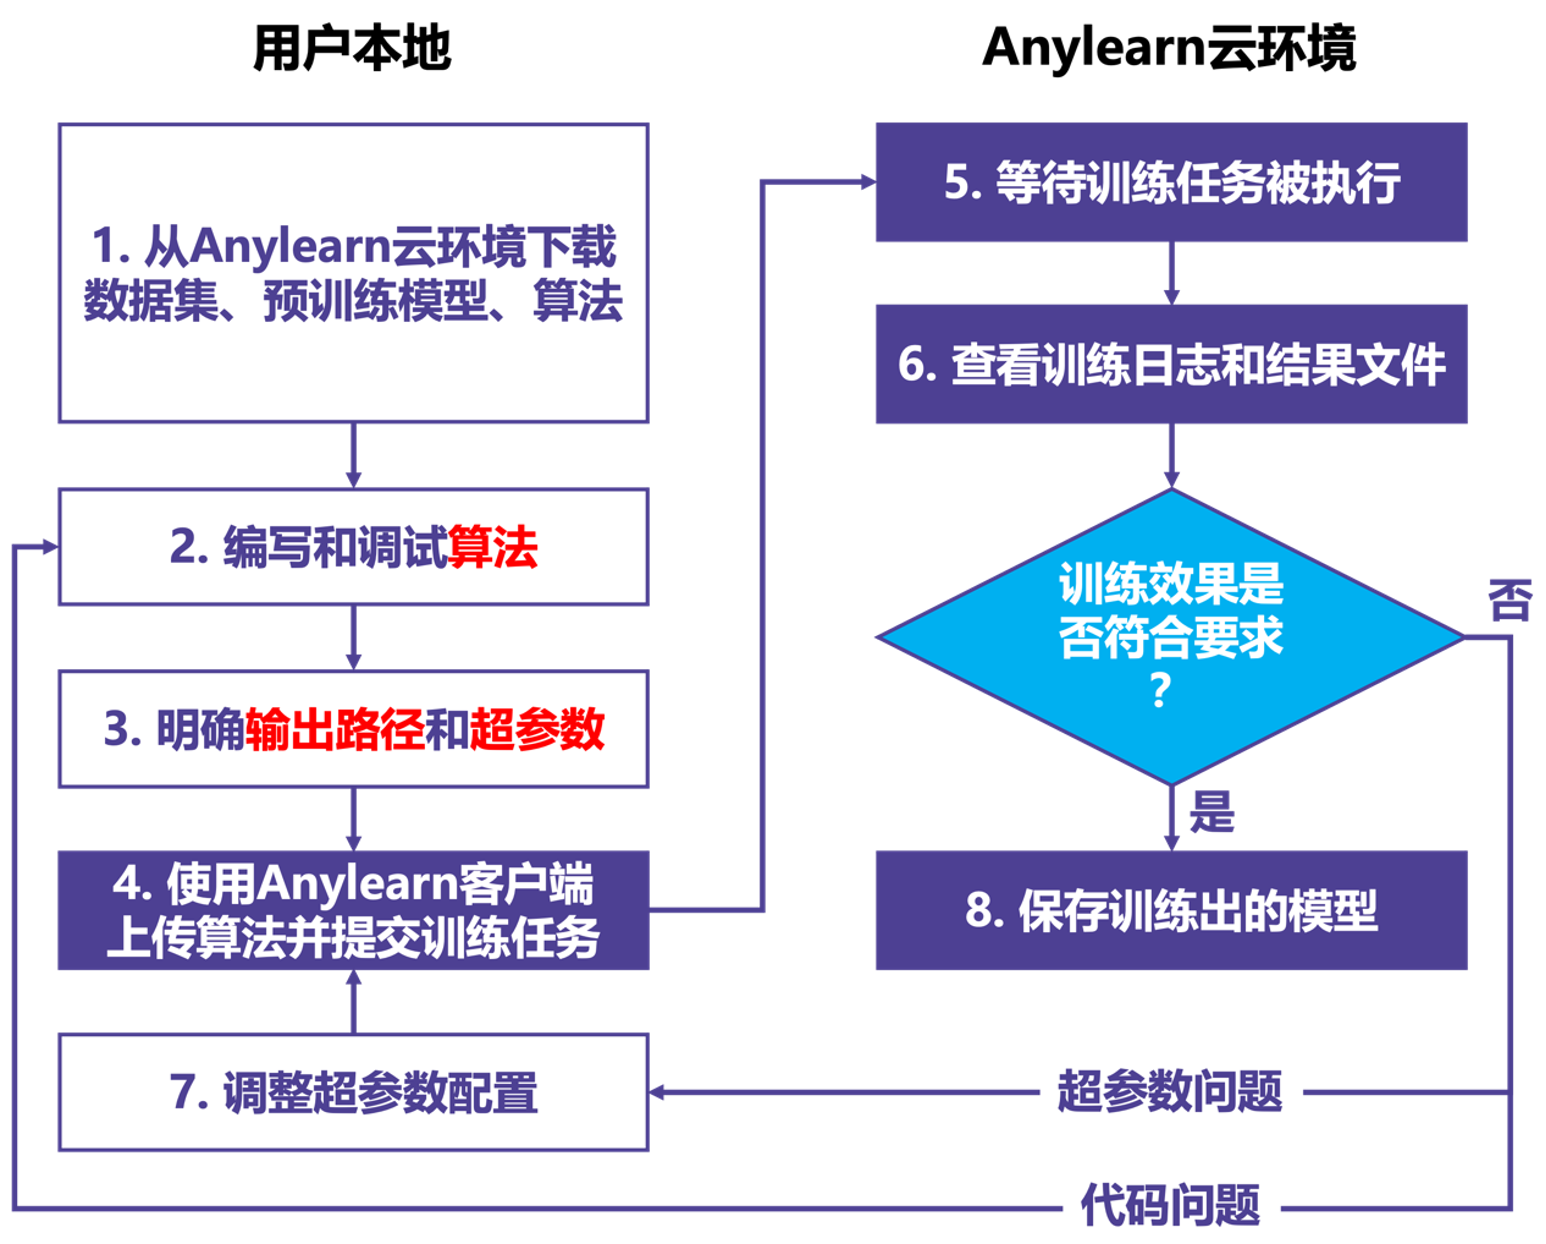
\includegraphics[width=0.8\linewidth]{anylearn-scenario2.png}
  \caption{Anylearn使用场景二:参与云环境中的项目}
  \label{fig:scenario2}
\end{figure}

(1)用户按照项目组要求,通过Anylearn交互网页将Anylearn云环境中的数据集、预训练模型和算法下载至本地。
由于网络条件有限,从Anylearn交互网页上下载较大规模的数据集和模型(依据经验,GB级以上即为大)通常非常缓慢,应当联系Anylearn系统管理员通过其他方式下载。

(2)用户在本地修改算法代码并调试,确保修改后的代码在本地使用上述数据集和预训练模型初步跑通训练和验证。

(3)后续步骤请参考场景一的步骤(4)至(9)。


\section{系统设计}

重点针对机器学习模型的研发效率问题,在业务层面上,Anylearn支持机器学习研发的过程管理、知识沉淀、模型迁移,满足资源统筹利用、团队高效协作等人工智能工程化需求;
在技术层面上,Anylearn采用了云原生的技术架构,以云原生领域的事实标准Kubernetes作为基础架构,充分融合网络应用系统和人工智能领域的开源生态,构建出全面容器化、模块化、可扩展、可伸缩、高可用的云原生机器学习平台。

\subsection{业务架构}
\label{sec:anylearnbusiness}

以研发管理的需求为导向,以模型研发的高效率、可追溯、可复现为总体目标,Anylearn的业务规划主要针对机器学习研发过程管理和资产管理两个方面。
图\ref{fig:anylearnbusiness}展示了Anylearn的业务总体架构。

过程管理方面,以数据挖掘和机器学习相关方法论\cite{Wir00, Ame19}为基础,聚焦模型研发紧密相关的数据准备、模型训练、超参数调优等环节,结合机器学习模型研发跨团队跨人员角色的特点,为算法工程师、数据科学家、软件工程师、领域专家、团队主管等研发人员提供组织管理、用户管理、过程分工、项目管理、可视化等管理能力。
资产管理方面,以数据集、算法族、模型库等资产为核心,通过研发任务进行串联,并基于数据对象抽象和数据实质存储之间的映射关系,实现所有资产元信息和资产存储的统一集约化管理,为团队提供资产的资产元信息管理、资产版本管理、关联关系管理、模型血统等管理能力,同时基于权限机制对团队提供资产共享协作的能力。

\begin{figure}
  \centering
  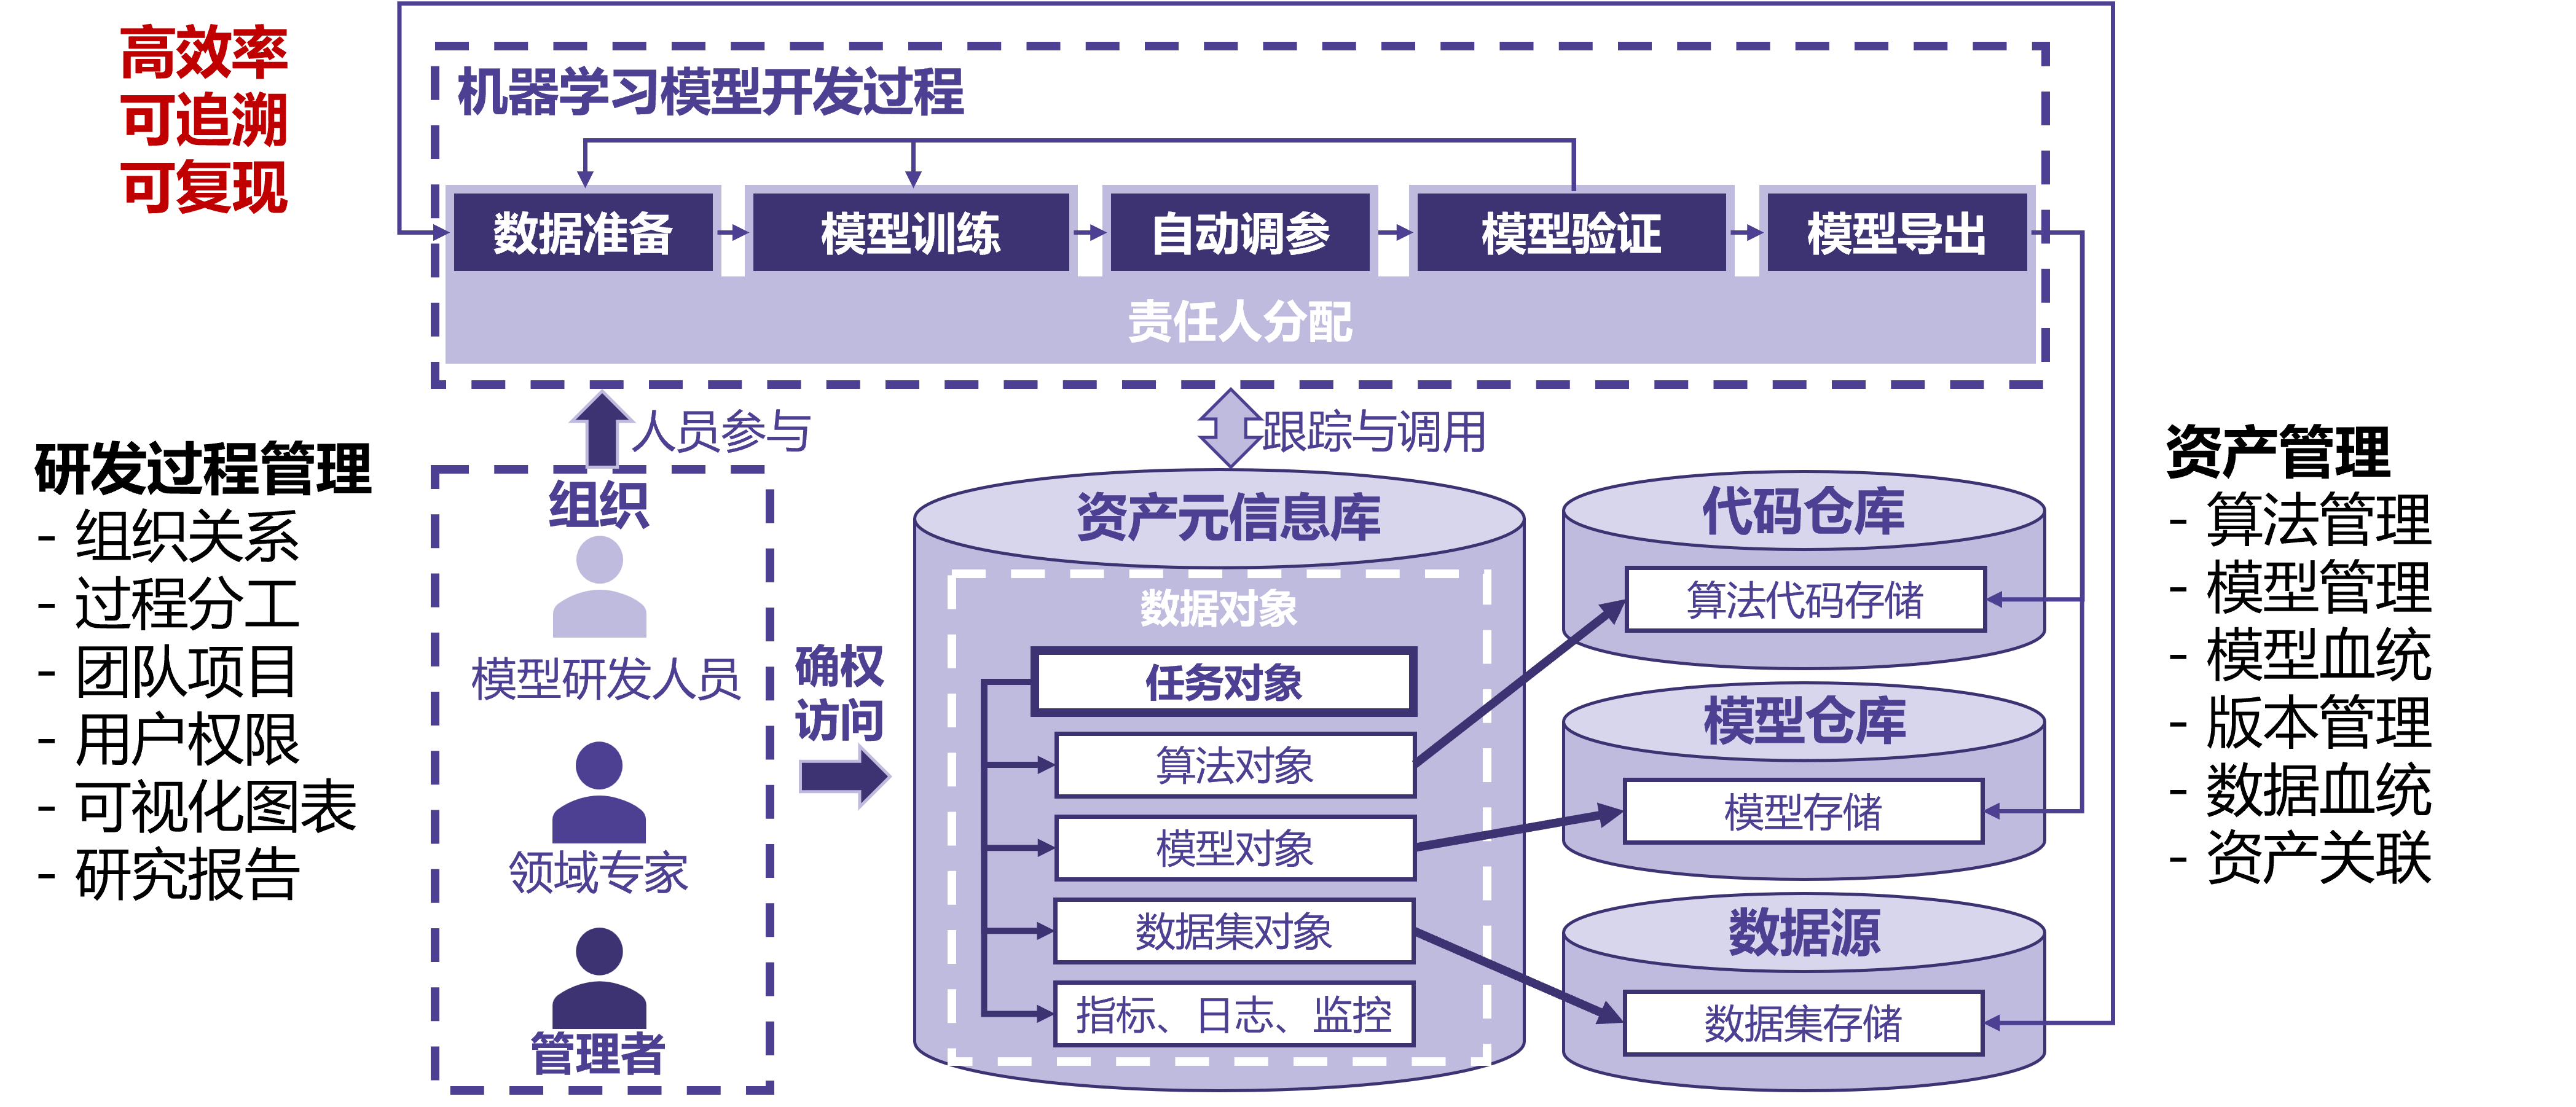
\includegraphics[width=0.98\linewidth]{anylearn-architecture-business.png}
  \caption{Anylearn业务总体架构}
  \label{fig:anylearnbusiness}
\end{figure}

\subsection{系统架构}

Anylearn在系统整体角度上看的架构如图\ref{fig:anylearnsys}所示。

\begin{figure}
  \centering
  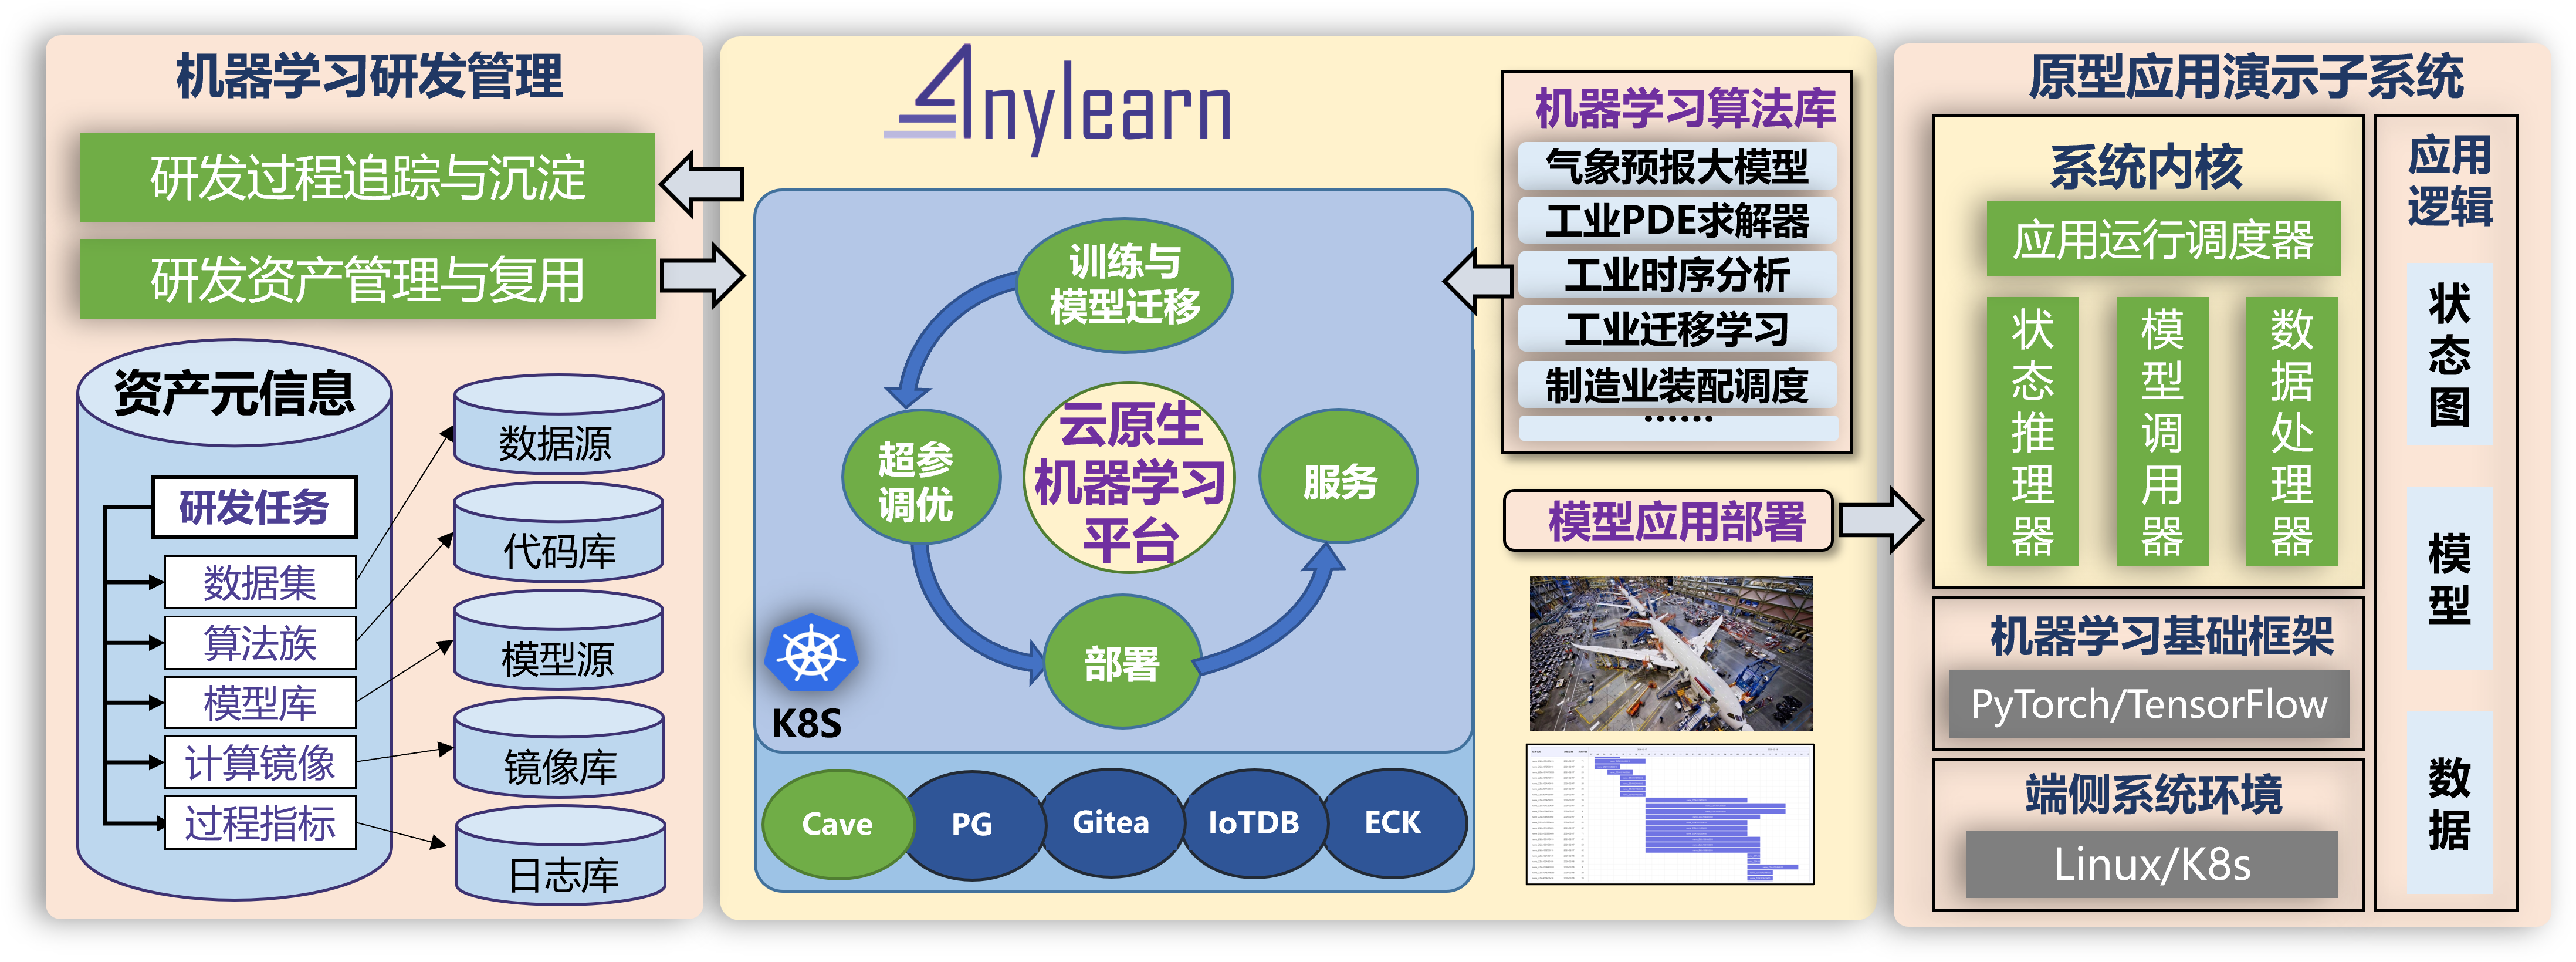
\includegraphics[width=0.98\linewidth]{anylearn-architecture-system.png}
  \caption{Anylearn系统总体架构}
  \label{fig:anylearnsys}
\end{figure}

对外,Anylearn提供以研发过程管理和研发资产管理为主的机器学习研发管理能力,如\ref{sec:anylearnbusiness}节所述。
对内,Anylearn基于Kubernetes基础架构和云原生开源生态技术栈,形成了训练验证、调参、部署、服务一体化的云原生机器学习平台,从概念上支撑并集成多个领域的算法库,包括气象大模型、时序大模型、工业仿真求解、智能调度等。
此外,机器学习模型的原型应用演示作为Anylearn的子系统为用户提供了模型应用的可视化展示和交互能力。


\subsection{功能架构}

Anylearn的功能架构围绕机器学习研发全流程展开,通过模块化设计支持高效的过程管理和资产管理,满足研发团队对复杂任务的需求,如图\ref{fig:anylearnfeatures}所示。

\begin{figure}
  \centering
  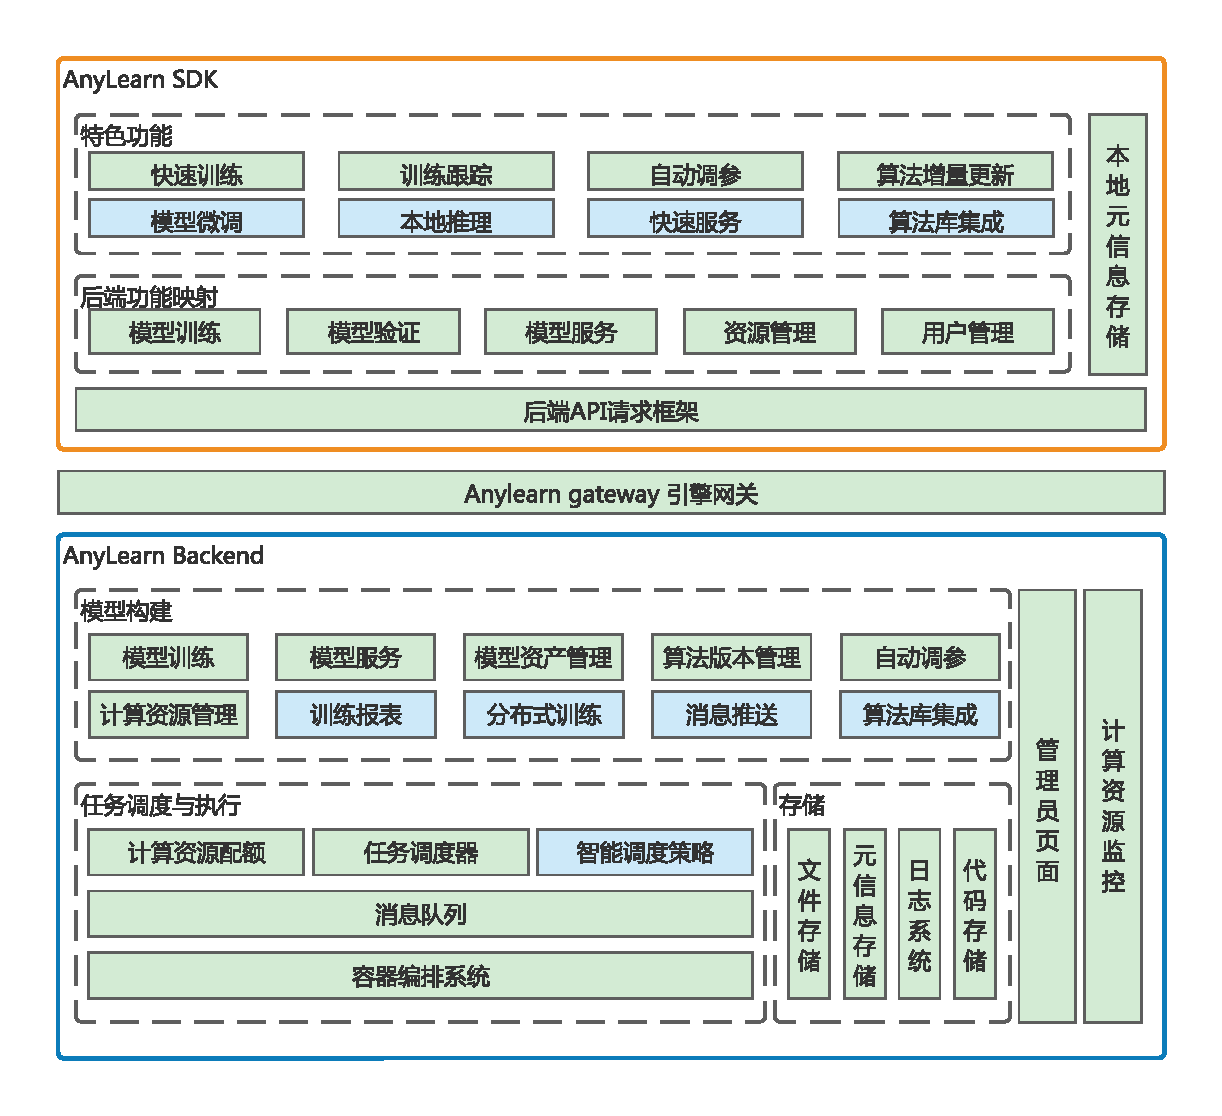
\includegraphics[width=0.8\linewidth]{anylearn-architecture-features.pdf}
  \caption{Anylearn功能架构}
  \label{fig:anylearnfeatures}
\end{figure}

平台的功能架构主要分为SDK、网关和后端三大部分。

Anylearn Python SDK主要用于用户端的功能接口和本地存储管理,包含特色功能和后端功能映射两部分。
特色功能包括快速训练、训练跟踪、自动调参、算法增量更新、模型微调、本地推理以及快速服务等,强调本地元信息的存储和高效执行。
而后端功能映射部分则提供模型训练、模型验证、模型服务、资源管理和用户管理功能,并通过后端API请求框架实现和后台服务的通信。

Anylearn gateway作为引擎网关,起到连接SDK和后端的桥梁作用,为前后端数据和功能流转提供支持。

Anylearn后端是整个系统的核心后台,主要分为模型构建和任务调度与执行两个部分。
在模型构建方面,涵盖了模型训练、模型服务、模型资产管理、算法版本管理、自动调参等功能,同时提供了计算资源管理、分布式训练、算法库集成以及消息推送等支持。
在任务调度与执行方面,通过智能调度策略和任务调度器对计算资源进行分配,依赖消息队列和容器编排系统完成任务的执行。
后端还具有完善的存储系统,包括文件存储、元信息存储、日志系统和代码存储等模块,并且配备管理员页面实现计算资源监控和管理。

\subsection{数据架构}

Anylearn的数据架构如图\ref{fig:anylearndata}所示。
数据模型的设计遵循叙述性(declarativity)原则\cite{Sch17}:资产表存储资产的元信息,而不是产生这些资产的代码文件,元信息的存储使得查询和分析更加简便,如果存储代码文件,会使得代码的版本追溯变得困难,并且难以发现代码中存在的错误。

\begin{figure}
  \centering
  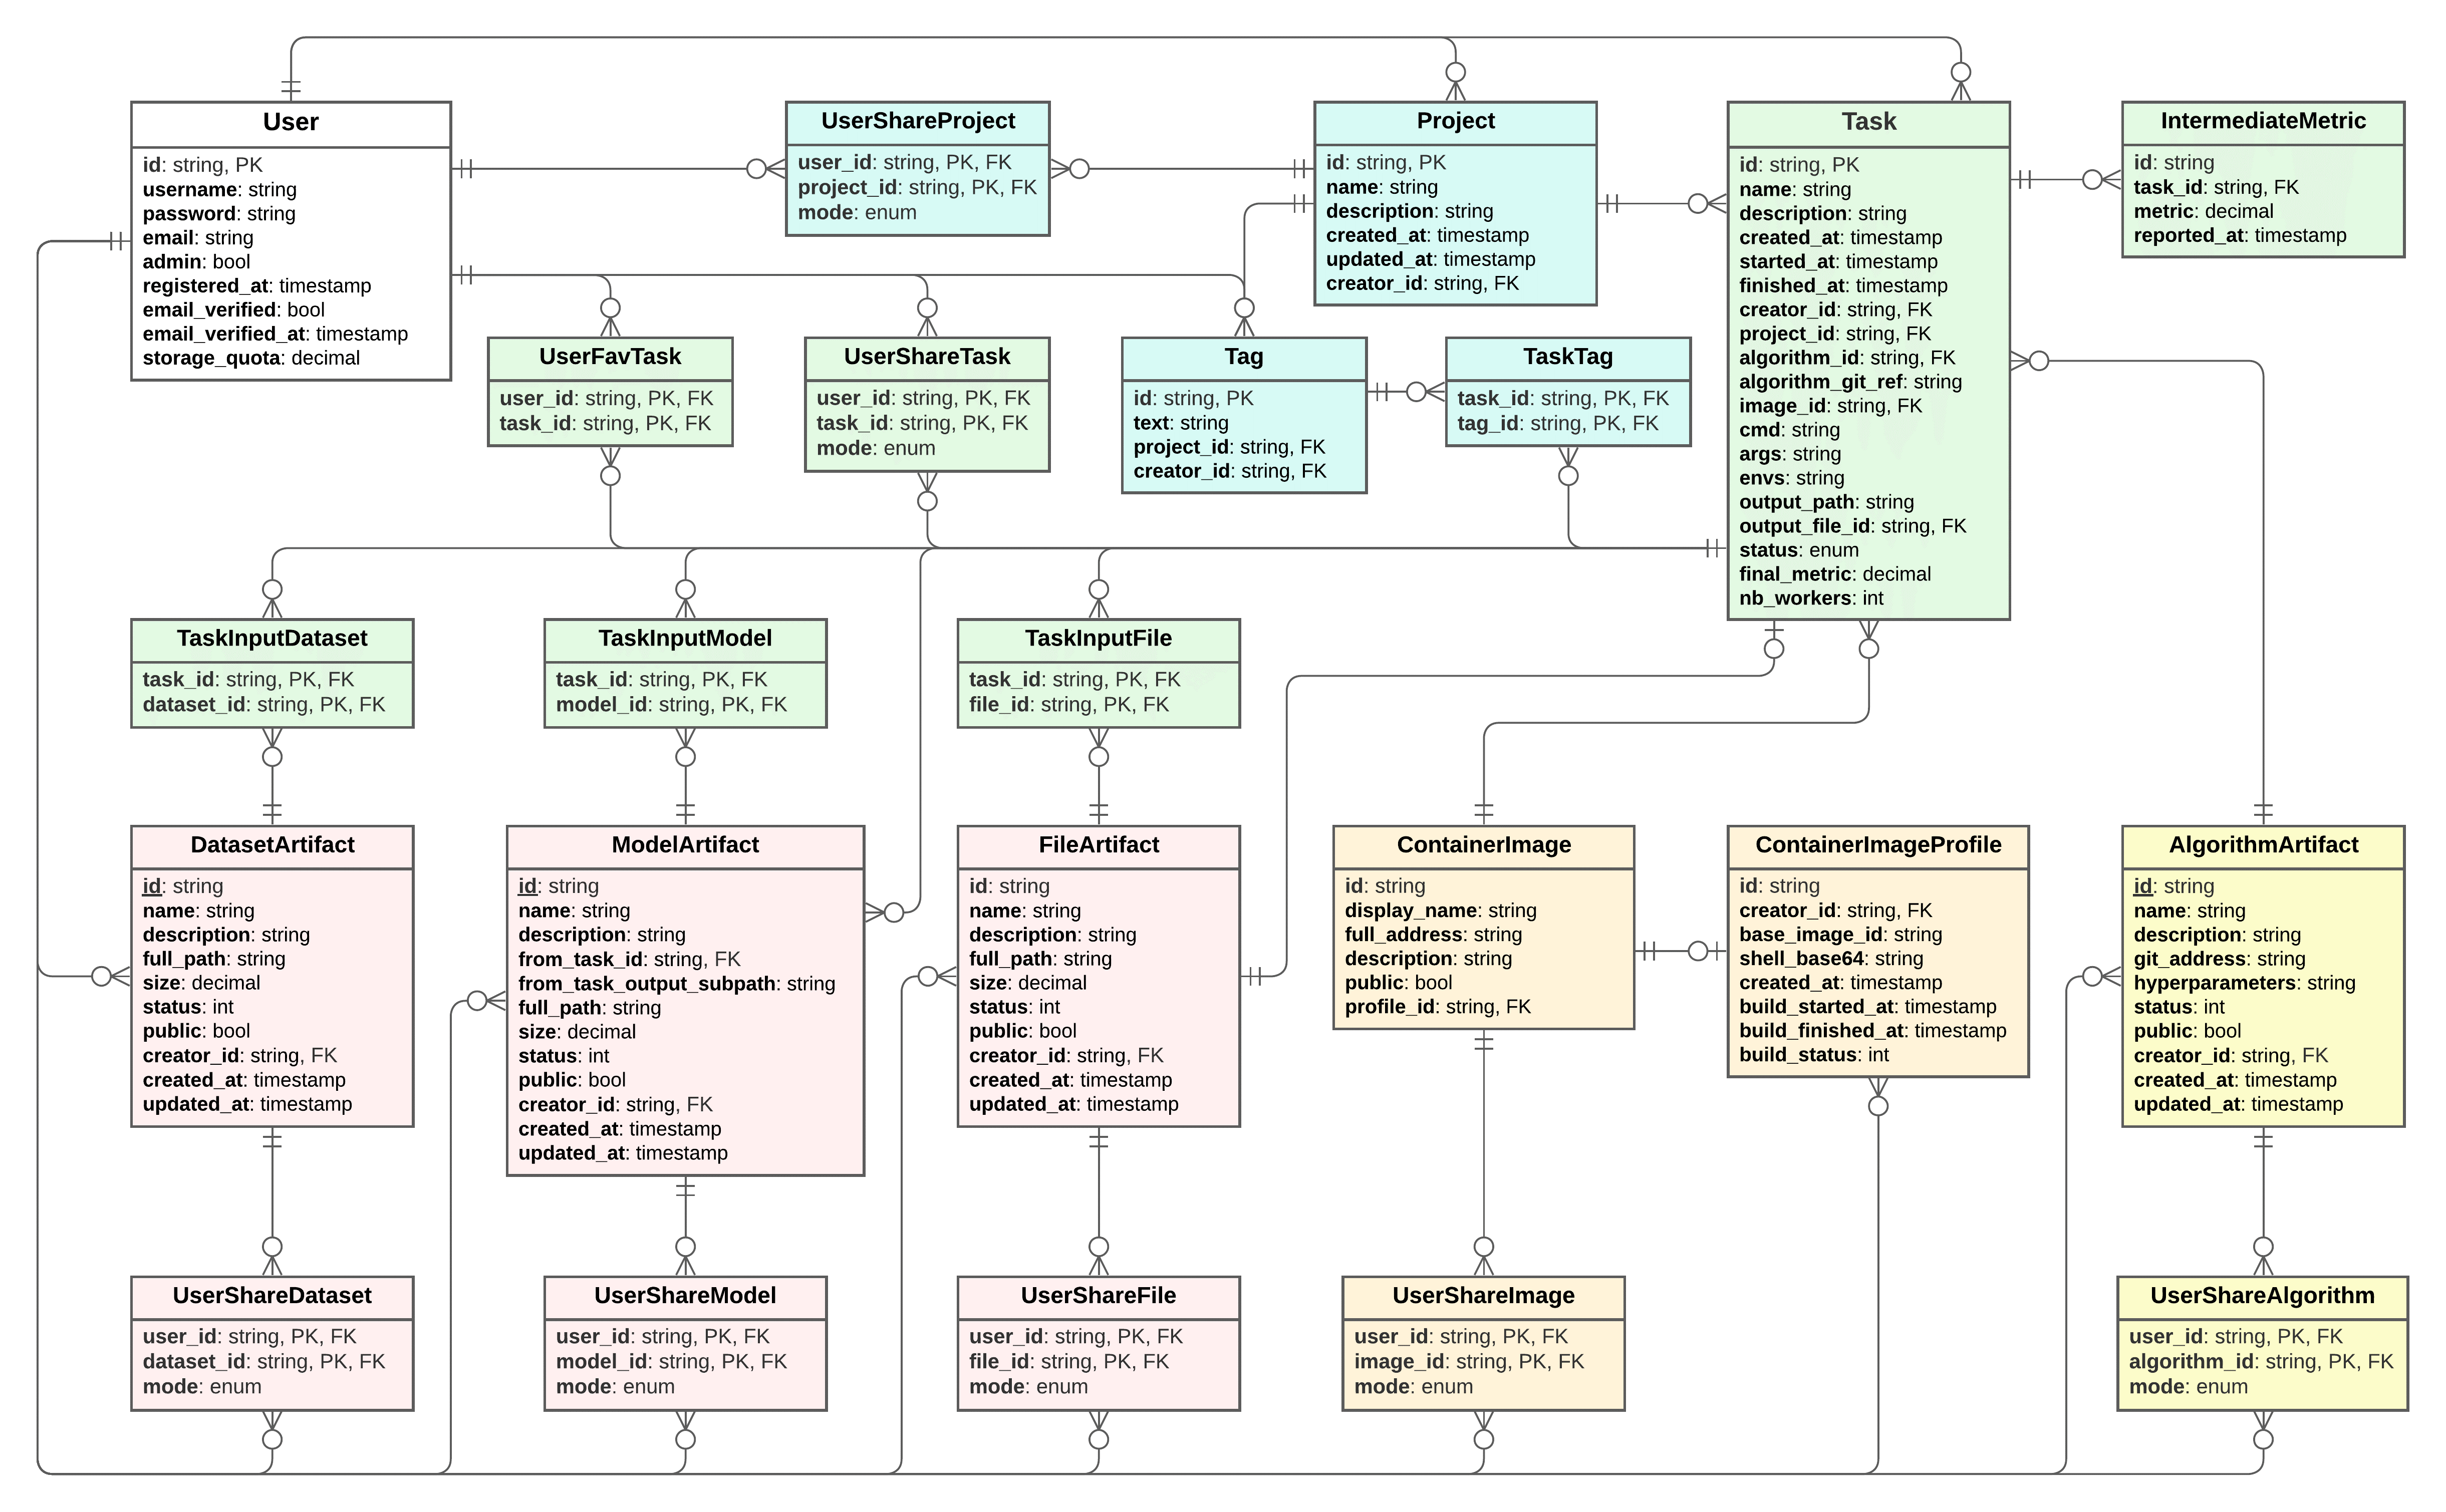
\includegraphics[width=0.98\linewidth]{anylearn-architecture-data.png}
  \caption{Anylearn数据模型架构}
  \label{fig:anylearndata}
\end{figure}

数据模型包含以下四大类数据表结构。

(1)用户表,包括存储用户信息的 User 表。
User表记录了用户名、密码、邮箱、注册时间、邮箱的验证情况,并用一个布尔变量记录该用户是否是管理员。

(2)项目相关表,包括存储项目信息的 Project 表、存储用户分享项目的 UserShareProject 表、存储项目标签的 Tag 表和存储任务标签的 TaskTag 表。
Project表记录了名字、描述、创建时间、更新时间、创建者。
Tag 表记录标签文本,通过外键和 User表和Project表成多对一关系。
TaskTag表作为关系表,使得Tag表和Task表成多对多关系,符合数据库设计的第三范式(3NF)。
UserShareProject 作为关系表,使得User表和Project表成多对多关系。

(3)任务相关表,包括存储任务信息的 Task 表、存储即时指标的 IntermediateMetric 表、存储用户点赞和分享任务的 UserFavTask 和 UserShareTask 表、存储任务输入的数据集、模型、和文件的 TaskInputDataset、TaskInputModel、TaskInputFile表。
Task表记录了任务名、描述、创建时间、启动时间、结束时间、创建者、所属项目、使用算法、算法仓库引用、使用镜像、启动命令、启动参数、环境变量、输出路径、输出文件、当前状态、最终指标等信息。
TaskInputDataset、TaskInputModel、 TaskInputFile 三者作为关系表,使得Task表和数据集、模型、文件这三类资产表成多对多的关系,从而记录了任务的资产血统信息,符合第三范式(3NF)。
Task表通过外键与ContainerImage、FileArtifact、AlgorithmArtifact成多对一的关系。
UserFavTask、UserShareTask、IntermediateMetric通过外键与Task表成多对一关系。

(4)资产相关表。
Anylearn的资产包括数据集、模型、文件、训练镜像和算法五类,根据资产的特点,可以分为以下三类:

(4.1)数据集、模型、文件。这三者都是以文件形式存储在本地磁盘上,数据表的字段相近,因此归为一类。该类包括了存储数据集、模型和文件元信息的 DatasetArtifact、ModelArtifact、FileArtifact表,存储用户分享数据集、模型和文件的 UserShareDataset、UserShareModel、UserShareFile表,这三张表作为关系表,使得三张资产表和User表成多对多关系。

(4.2)训练镜像。镜像由docker由进行管理,这类表包括存储镜像元信息的 ContainerImage、存储自定义镜像元信息的ContainerImageProfile 表、存储用户分享镜像的 UserShareImage表。ContainerImage表记录了展示名、完整地址、描述,并用一个布尔变量标识公开性。ContainerImageProfile表记录自定义镜像的创建者、基础镜像、base64编码、创建时间、构建开始时间、构建结束时间、构建状态,与User表成多对一关系,与ContainerImage表成一对一关系。UserShareImage表作为关系表,使得ContainerImage表和User表成多对多关系。

(4.3)算法。算法代码文件使用gitea进行版本管理,该类包括存储算法元信息的 AlgorithmArtifact表、存储用户分享算法的 UserShareAlgorithm 表。UserShareAlgorithm表作为关系表,使得AlgorithmArtifact表与User表成多对多关系。

根据数据表的设计,Anylearn的数据模型能够满足以下几点特性。

(1)存储资产元信息。 
数据模型包含相应的表(DatasetArtifact,ModelArtifact,FileArtifact,AlgorithmArtifact、ContainerImage)来存储数据集、模型、文件、算法、镜像这五种资产的元信息,前四者共有的元信息有资产的名字、描述、状态、公开可见性、创建者、创建时间、更新时间,数据集、模型、文件特有的元信息包括实际存储路径、文件大小,模型的元信息还包括一个外键记录对应任务,算法特有的元信息包括git地址、超参数。

(2)支持资产追溯。
上述五类资产和任务是相关联的,每个任务关联一个算法,另外关联一个或多个数据集、模型、文件,任务和镜像是多对一关系,因此可以通过查找任务关联的方式追溯各类资产。

(3)支持用户协作。
UserShareDataset、UserShareModel、UserShareFile、UserShareImage、UserShareAlgorithm 五张关系表存储了用户将自己管理的数据集、模型、文件、镜像、算法分享给其他用户的信息,方便查询和修改。

(4)保存执行环境。
ContainerImage和ContainerImageProfile表存储训练任务的镜像信息,得以保存每次训练任务的执行环境,避免了操作系统、驱动或依赖库不同可能带来的可复现性问题。

(5)支持自定义标签。
Tag表存储了用户给项目贴的标签,TaskTag表存储了项目中各个任务含有的标签,这样的设计使得用户可以自建标签索引,方便用户对项目和任务进行搜索,实现了跨资产检索的高级管理功能。

\subsection{技术架构}

在技术实现的层面上,Anylearn采用了主流的C/S架构,组件层级主要分为客户端、服务端、系统软件基础设施和云原生基础平台。
客户端主要包括Web页面、Python SDK和命令行工具。
服务端主要包括负责元信息和存储管理的管理侧后端、负责任务调度和执行的执行侧后端、容器运行时、文件存储等组件。
系统软件基础设施层主要包括关系型数据库、时序数据库、消息队列、Git平台、日志套件和监控套件。
底层云原生基础平台则是云原生的事实标准Kubernetes。
整体如图\ref{fig:anylearntech}所示。

\begin{figure}
  \centering
  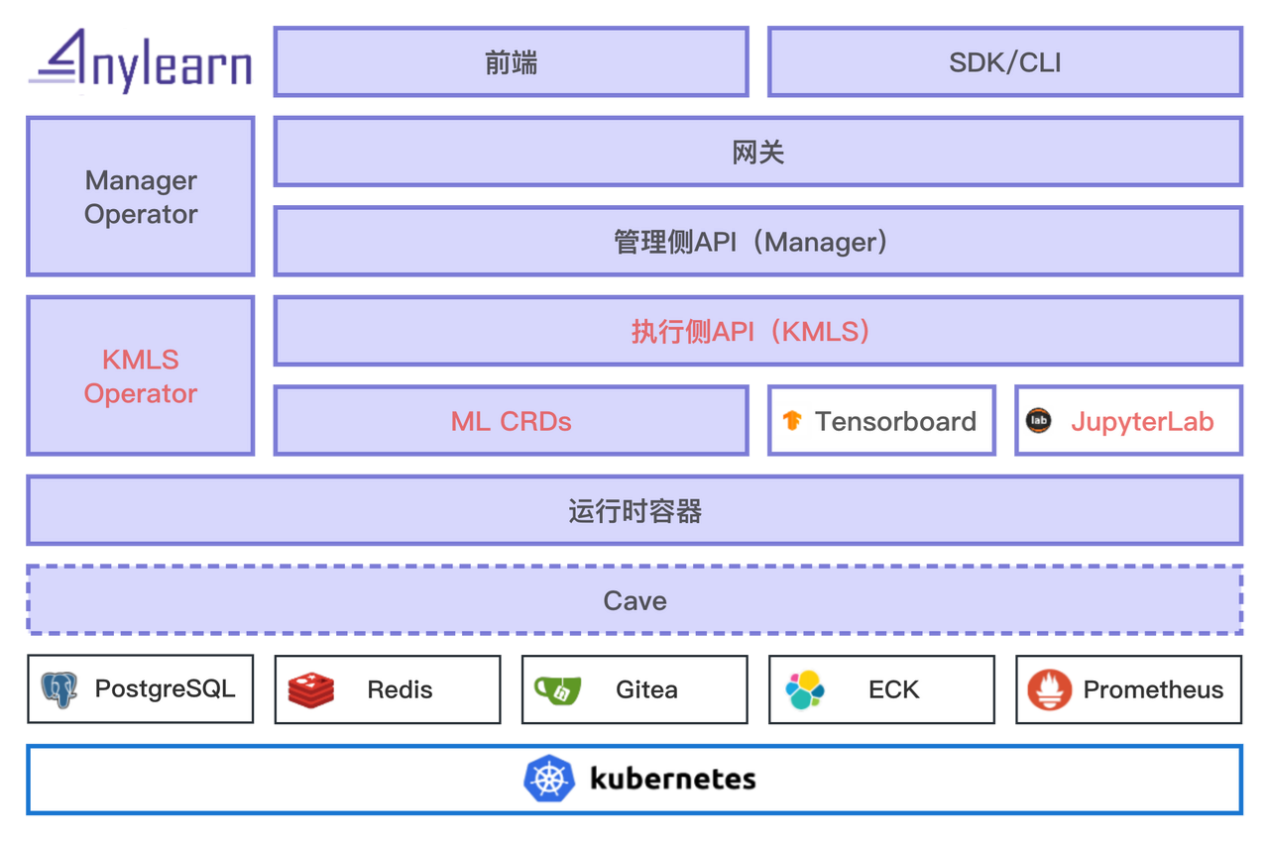
\includegraphics[width=0.8\linewidth]{anylearn-architecture-tech.png}
  \caption{Anylearn技术组件架构}
  \label{fig:anylearntech}
\end{figure}

前端Web页面采用了Vue2框架,实现了客户端路由、状态管理、文件目录结构预览、代码预览、图像预览、控件拖拽、图表可视化等基础技术能力,支撑了Anylearn直接面向用户的业务功能,包括用户注册登录、任务信息展示、资产信息展示、主管监控页面等等。
与后端通过RESTful API进行通信,开发阶段可通过URL代理对接不同的服务端环境。

Python SDK本质上是对RESTful API的封装,提供了更加友好的Python接口,方便用户在编程环境中调用Anylearn的服务端功能,可灵活支持与其他业务系统的集成。
此外,Python SDK中还特别提供了面向算法开发者的快速训练接口,可以通过编写简单的Python脚本调用一个函数即可将本地算法上传至Anylearn云环境并提交训练任务,对算法开发调试阶段的快速迭代试错提供了有力支撑。

命令行工具是基于Python SDK采用Click命令行框架实现的,提供了一些简单的命令行接口,方便用户在终端环境中调用Anylearn的服务端功能,例如:上传数据集、下载模型、查看计算资源情况等。

管理侧后端采用了Python的Flask框架实现,负责元信息和存储管理,包括用户管理、项目管理、任务管理、资产管理、标签管理、用户权限等功能。
此外,管理侧还负责对接底层文件存储、关系型数据库、时序数据库、消息队列、Git平台、日志套件和监控套件,支撑资产存储管理、元信息管理、训练过程数据管理、任务执行代理、算法代码管理、训练日志管理和系统监控管理等技术能力。
在部署形态上,管理侧采用了Kubernetes Operator的应用开发范式,通过CRD和控制器的方式实现了管理侧后端的自动化部署以及基础的容错和故障恢复。

执行侧后端是完全云原生的服务,采用了Kubernetes Operator的应用开发范式,将在线开发、训练、原型应用(推理服务)、自定义镜像构建、训练过程跟踪、超参数调优、文件压缩(模型、数据集、结果文件等)等作业抽象成Kubernetes的Deployment长时服务或Pod短时任务,并通过CRD和控制器进行启停维护和管理。

执行侧向下直接依托于容器运行时和一系列容器镜像。
Anylearn在原理上采用通用的容器化作业执行,理论上可支持所有可在容器内运行的机器学习计算框架,如PyTorch、TensorFlow、MindSpore、PaddlePaddle、XGBoost等。
根据当前用户的实际需求,Anylearn提供了以PyTorch为主的一系列基础镜像,并支持用户基于这些镜像构建自定义镜像,以满足用户对特定框架、特定库、特定环境的需求。

存储方面,Anylearn底层对NFS进行了封装形成了Cave存储组件,并通过Kubernetes的Deployment和Service进行部署,形成文件存储集群,支持容器内远程挂载形成持久化存储。
此外,Anylearn在管理侧后端的Operator中深度集成了Cave的部署管理,可以支持目录级别的NFS节点启动,并支持动态扩缩容。
然而,Cave属于轻量化封装组件,并未针对分布式存储的数据可用性、数据冗余、读写性能等方面进行实现。
在快速部署和小规模业务场景下可以屏蔽存储层的复杂性,但在大规模并发训练任务的场景下可能会成为瓶颈。

系统软件基础设施方面,Anylearn采用了PostgreSQL作为关系型数据库,管理元信息和关联关心;采用IoTDB作为时序数据库,存储和管理训练过程跟踪数据;采用Redis作为消息队列和中间件,传递任务执行信息,解耦管理侧与执行侧;采用Gitea作为Git平台,负责管理算法代码库和版本控制,与管理侧深度集成,可独立于用户算法本身的Git仓库互不影响,同时又能精准记录每一次训练相关的代码变更;采用ECK+EFK作为日志套件,Prometheus作为监控套件。


\section{线上环境}

“实践是检验真理的唯一标准”这一理念对于软件尤为重要,敏捷开发方法论中也强调了用户反馈对软件迭代的意义。
为了验证Anylearn的能力并持续打磨其功能性能,2021年7月起,Anylearn在大数据系统软件国家工程研究中心的私有云进行了部署,作为一套公开长活的线上系统对外提供服务,供软件学院、研究中心以及其他相关科研团队使用。

\subsection{集群架构}
Anylearn线上环境中配备了11台高性能GPU服务器,每台服务器配备4张GPU,共计44张,包括24张NVIDIA A100(其中20张为40G显存版,4张为80G显存版)和20张NVIDIA GeForce RTX 3090。
Anylearn依托私有云的网络环境,通过搭建Kubernetes集群池化纳管所有GPU服务器。
Kubernetes集群中使用了私有云的3台虚拟机作为主节点形成控制面,并通过内网负载均衡器与GPU服务器连通,实现了集群的高可用,即任意2个主节点下线均不影响集群任何功能的访问。
集群节点的架构如图\ref{fig:cluster}所示。

\begin{figure}
  \centering
  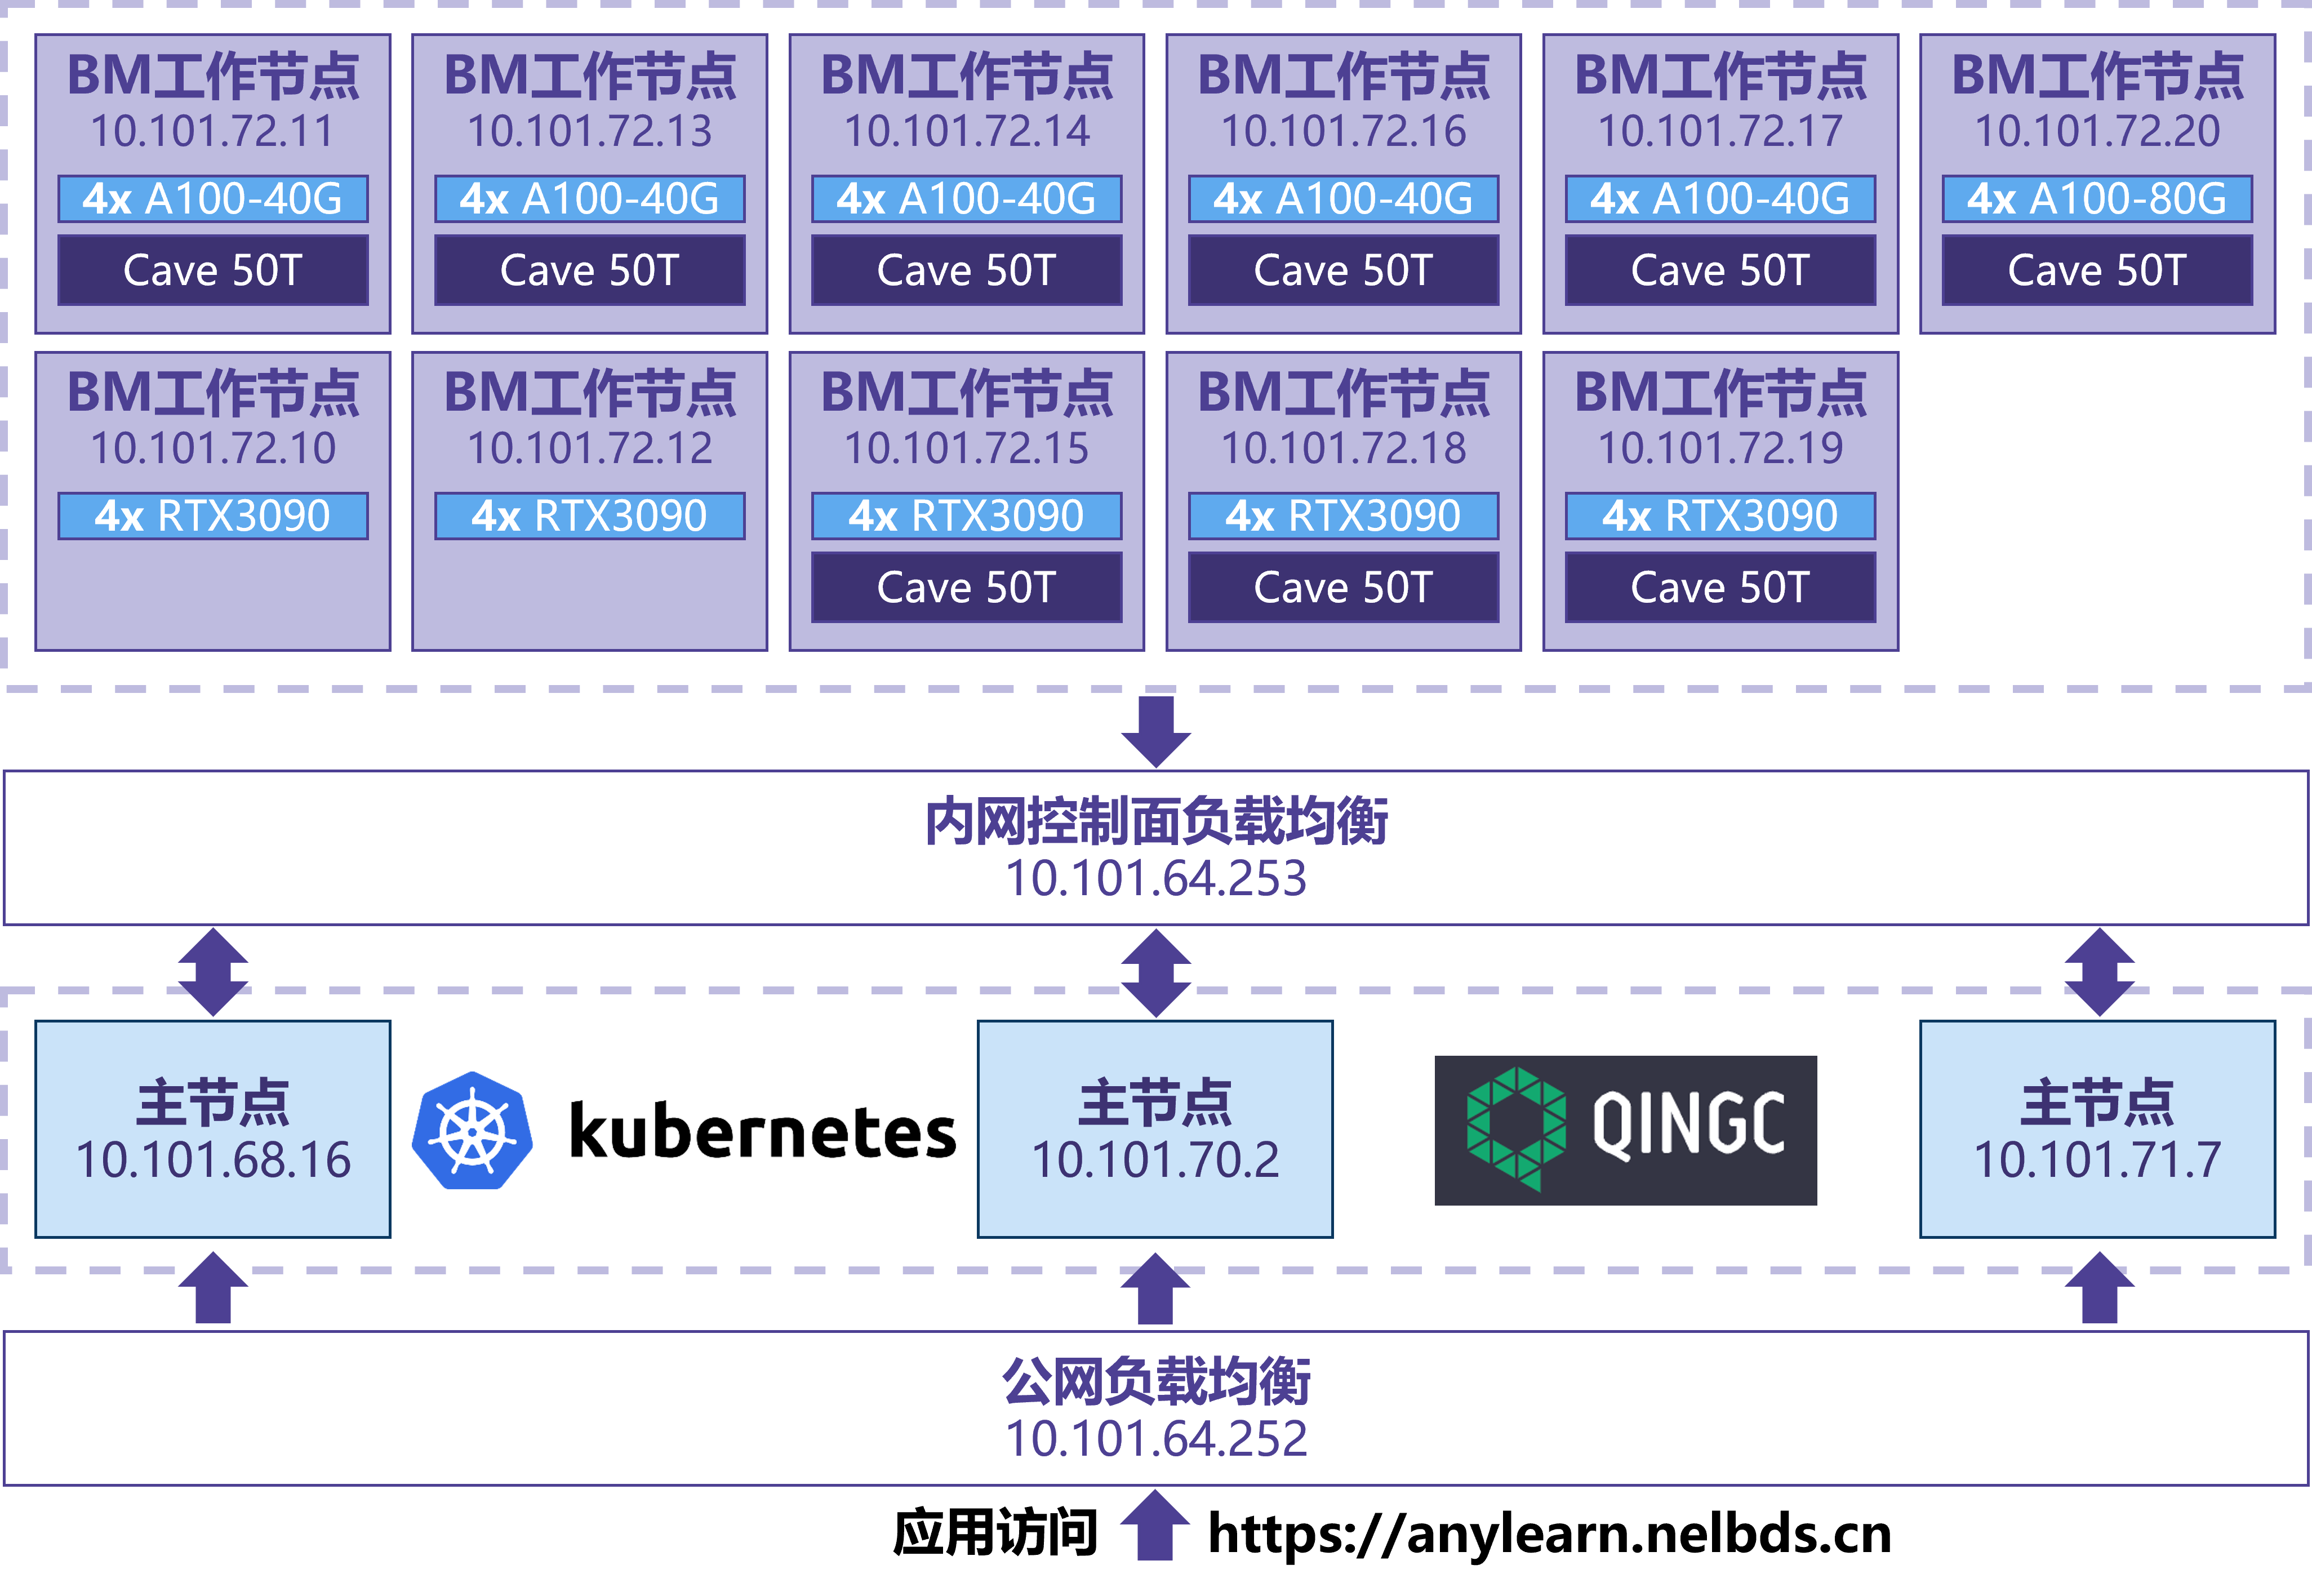
\includegraphics[width=0.98\linewidth]{anylearn-cluster-structure.png}
  \caption{Anylearn线上环境集群架构}
  \label{fig:cluster}
\end{figure}

集群架构经历过7次较大的变动:
(1)2021年7月首次部署时,集群中包含了9台GPU服务器,其中2台未配备GPU,故用作Kubernetes集群控制面的双主节点形成伪高可用架构;
(2)2021年9月,集群中GPU齐备,数量为36张,原用作主节点的2台GPU服务器应当专用于GPU算力负载,不再适合分散其负载能力到控制面,故使用3台私有云虚拟机作为集群主节点,形成真正高可用的集群控制面; 
(3)2022年6月,由于集群证书配置问题导致集群不可用,重新部署了集群并调整了主节点虚拟机的配置;
(4)2022年1月,集群中新增了1台GPU服务器,包含4张NVIDIA GeForce RTX 3090,GPU数量增至40张,扩展操作仅为数条命令,且未影响任何线上业务;
(5)2023年5月,集群中新增了1台GPU服务器,包含4张NVIDIA A100(80G显存版),GPU数量增至44张,扩展操作仅为数条命令,且未影响任何线上业务;
(6)2023年8月,Kubernetes版本从1.21.2逐小版本升级至1.28.1(即1.21.x升级至1.22.x再升级至1.23.x,以此类推直到1.28.1);
(7)2024年3月,由于作为集群主节点的3台私有云虚拟机Linux内核版本过低(4.15),影响了集群网络插件的性能,故重新创建了3台安装了较新版本的Linux内核(5.4)的虚拟机,并将主节点逐一替换,未影响任何线上业务。

\subsection{使用情况}
截至2024年11月14日,Anylearn线上长活环境累计执行了8万8千余次实验,任务执行时长超59万小时,并积累了大量的研发资产,包括近600个共超220TB的数据集、近2万份算法代码和近1600个成品模型。
科研方面,Anylearn支撑了“风清”和“风雷”气象大模型的研发、Timer时序大模型的研发与演示、飞机装配智能调度模型研发与演示等重点项目和重大工程的研究工作,获得了研发人员的高度认可,相关成果发表在《自然》\cite{Zha23}、《中国科学:信息科学》\cite{Zho24}等顶尖期刊。
教学方面,Anylearn支撑了深度学习、大数据基础、软件工程实践等研究生课程和本科生课程,作为模型训练平台为学生提供作业所需的计算资源、训练验证功能、数据集和预训练模型,并为助教和教师提供了作业监管能力。

\begin{table}
  \centering
  \caption{Anylearn线上环境历年使用情况统计}
  \begin{tabular}{crrrrr}
    \toprule
    \multicolumn{1}{c}{年份} & \multicolumn{1}{c}{任务数量} & \multicolumn{1}{c}{执行时长} & \multicolumn{1}{c}{数据集数量} & \multicolumn{1}{c}{算法族数量} & \multicolumn{1}{c}{模型数量} \\
    \midrule
    2021 & 7179 & 26977 & 39 & 619 & 42 \\
    2022 & 27137 & 140655 & 224 & 4715 & 791 \\
    2023 & 35410 & 271001 & 203 & 6336 & 526 \\
    2024 & 18987 & 151588 & 127 & 6993 & 240 \\
    \textbf{总计} & \textbf{88713} & \textbf{590221} & \textbf{593} & \textbf{18663} & \textbf{1599} \\
    \bottomrule
  \end{tabular}
  \label{tab:stats}
\end{table}

表\ref{tab:stats}展示了Anylearn线上环境历年使用情况统计。
其中,2021年系Anylearn集群上线初期,且运行时间仅不到半年,任务数量和执行时长较少。
2022年到2023年是上述科研工作的集中攻关时期,Anylearn整体使用量处于明显的增长态势,尤其体现在任务数量和任务执行时长上,说明Anylearn的功能性能得到了用户的认可,并且在持续完善中。
今年,作为Anylearn线上环境主要用户群的软件学院机器学习组,研究方向逐渐向大规模参数模型发展。
Anylearn集群受限于总体算力和网络带宽,不足以支撑全部的研发工作,因此部分模型训练和验证的任务转向校外算力中心进行,截至11月14日,整体使用量有所下降。


\section{用户案例}

本文以基于雷达回波外推的短临强降水预测大模型研究工作为例,展示了Anylearn在科研工作中的应用。

气象雷达是对大气的重要观测手段,雷达的回波可以很好地描述大气云层的物理状态,从而在机理层面上推测出降雨、雷暴、冰雹等天气情况。
雷达回波外推是模拟未来若干时刻上的雷达回波,推演云层的变化情况和趋势,是气象及气候分析领域的关键技术之一。
随着近些年深度学习技术在视觉和预测等领域的蓬勃发展,基于深度学习的雷达回波外推顺理成章地得到了学术界的广泛关注\cite{Zha23}。
雷达回波数据本质上具有时间和空间的双重属性,其外推任务的核心科学问题即时空数据的预测问题,属于当前机器学习学术界的前沿问题,需要系统化的团队合作才能高效地开展其研究工作。

清华大学软件学院的机器学习研究组针对雷达回波外推这一难题展开了重点攻关,并研制出了效果显著的深度学习模型。
Anylearn在其中发挥了重要的作用,主要体现在支撑雷达数据处理、管理模型的开发迭代、管理实验、通过实时预览辅助模型效果的分析等方面。

\subsection{雷达数据处理}
对于不同的模型研发方案,这些数据集需要进行大量的数据预处理方能进行模型的训练、验证和测试。
然而,深度学习的科研工作一般不以这类数据处理工作为核心贡献,因此在管理和执行层面上对其重视程度不足。
研发人员往往仅在原始数据上运行一些临时编写的数据处理脚本,并将处理后的数据重新保存起来,而经常忽视了数据处理脚本的版本控制、原始数据集的一致性以及处理结果、算法、原始数据集三者间的关联,可能会造成训练数据来源不明确、关键的数据处理方案遗失,进而导致模型效果无法客观评价、模型泛化能力无法保证等重大问题。

学术界常用的雷达回波公开数据集包括MRMS\cite{Smi16}、英国数据集\cite{Rav21}等,格式一般为图像文件PNG或气象领域专用的GRIB。
雷达回波外推深度模型的技术难度高,需要多名研发人员分工合作,由专人负责数据收集与处理、模型方案设计、实验设计与执行等工作,数据集也需要在不同的研发人员之间流转,若缺乏有效的交互和管理手段,则很容易形成瓶颈。
此外,模型实验通常需要在十几、几十台位于不同机房或数据中心的GPU服务器上同时进行,因此需要研发人员将上述数据集拷贝到不同服务器上。
当数据处理方式变更时,为保证实验中的数据一致性,所有拷贝的数据集均需相应变更,工作复杂度高、重复劳动多、管理难度大。

\begin{figure}
  \centering
  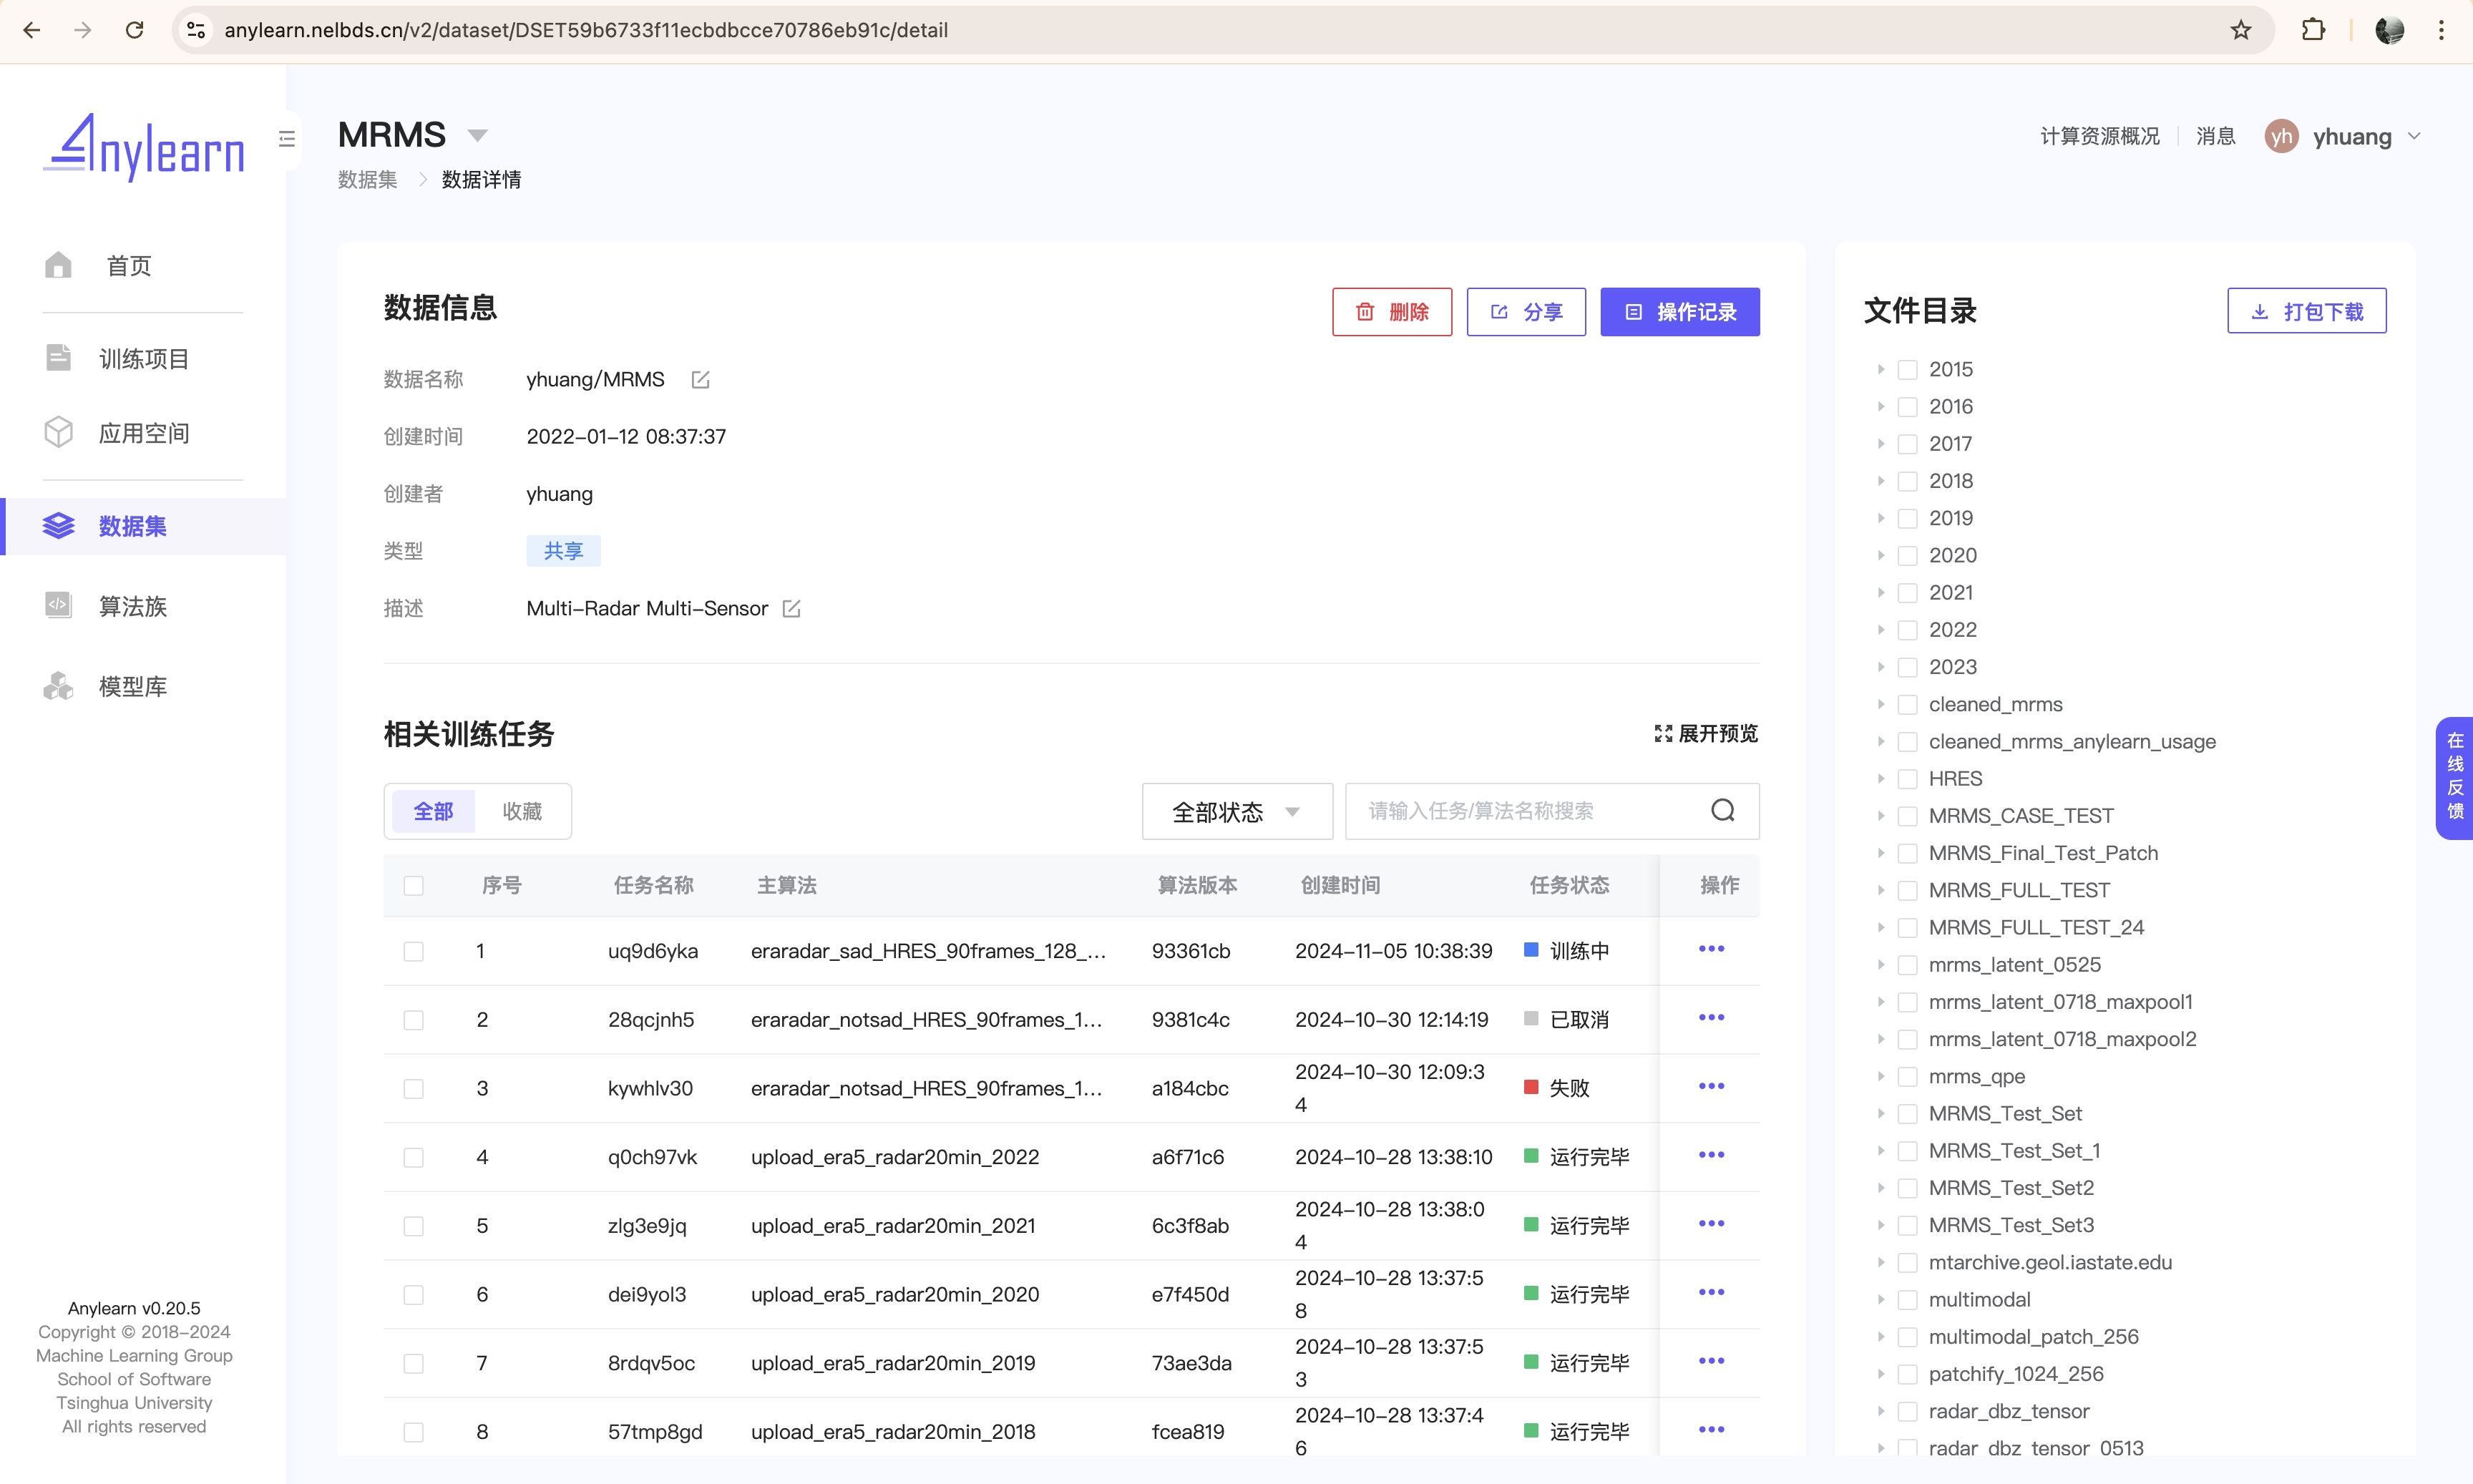
\includegraphics[width=0.98\linewidth]{mrms.jpg}
  \caption{Anylearn中的MRMS数据集}
  \label{fig:mrms}
\end{figure}

Anylearn的任务管理和资产管理可以有效地避免上述问题。
Anylearn底层的中心化文件存储可以保障数据处理、训练、验证等任务在不同节点执行时均可访问同一份数据集,无需在不同服务器上手动拷贝数据集。
负责数据处理工作的研发人员将数据处理脚本作为算法提交到Anylearn中进行管理和版本控制,确保数据处理方案不会遗失,同时也可以通过算法共享使团队内的其他研究人员了解数据处理过程的具体实现,促进沟通和讨论。
通过Anylearn数据处理任务在原始数据集上运行数据处理脚本并独立持久化存储处理后的数据,将脚本、原始数据集和处理后的数据集串联起来,满足后续的查询、检索、追溯等管理需求。
处理后的数据集可以作为数据处理任务结果共享给下游负责模型训练、验证、测试的研发人员,也可以写回原始数据集并共享给团队成员,满足团队协作需求。
所有雷达回波原始数据集以及处理后的数据集均通过Anylearn进行集约式的存储和管理,形成可追溯、可更新、可复用的数据集资产。
后续的模型训练、验证、测试等研发任务均以这些数据集资产为输入,能够以数据为中心地完整关联出模型研发过程中的各个阶段。

\subsection{模型开发迭代}
雷达回波外推模型研发的探索性强,需要基于不同的设计方案进行模型训练和效果验证,并不断迭代调整方案,在此过程中的实验记录格外重要。
由于缺乏便捷的实验记录工具,部分研发人员仍依赖电子表格手动记录实验,不仅效率低下,还容易遗漏重要数据。
人工记录的实验信息具有主观性,因人而异,在面临多人协作的使用场景时,需要人为制定记录规范才能较好地规避冲突,限制了沟通和讨论的效率。
此外,模型迭代的过程也是不断修改算法代码的过程,由此产生大量隐式的算法版本,很难通过人工记录的方式留存下每一次细微的代码变更并与训练结果形成关联,很容易导致方案的遗失。

使用了Anylearn,雷达回波外推模型研制过程中的上万次实验运行的元信息和实验方案代码均被自动化地记录了下来,确保每一次实验均可追溯的同时,省去了人工记录的工作量,避免了人工记录的谬误。
图\ref{fig:radartasks}展示了Anylearn中记录的雷达回波外推模型研发团队一位核心骨干成员的部分实验任务列表,最早的任务可追溯到2021年12月。
所有实验任务所使用的数据集、算法版本、超参数以及产生的结果等关键信息都被完整地持久化,便于研发人员溯源、交流、复盘。

\begin{figure}
  \centering
  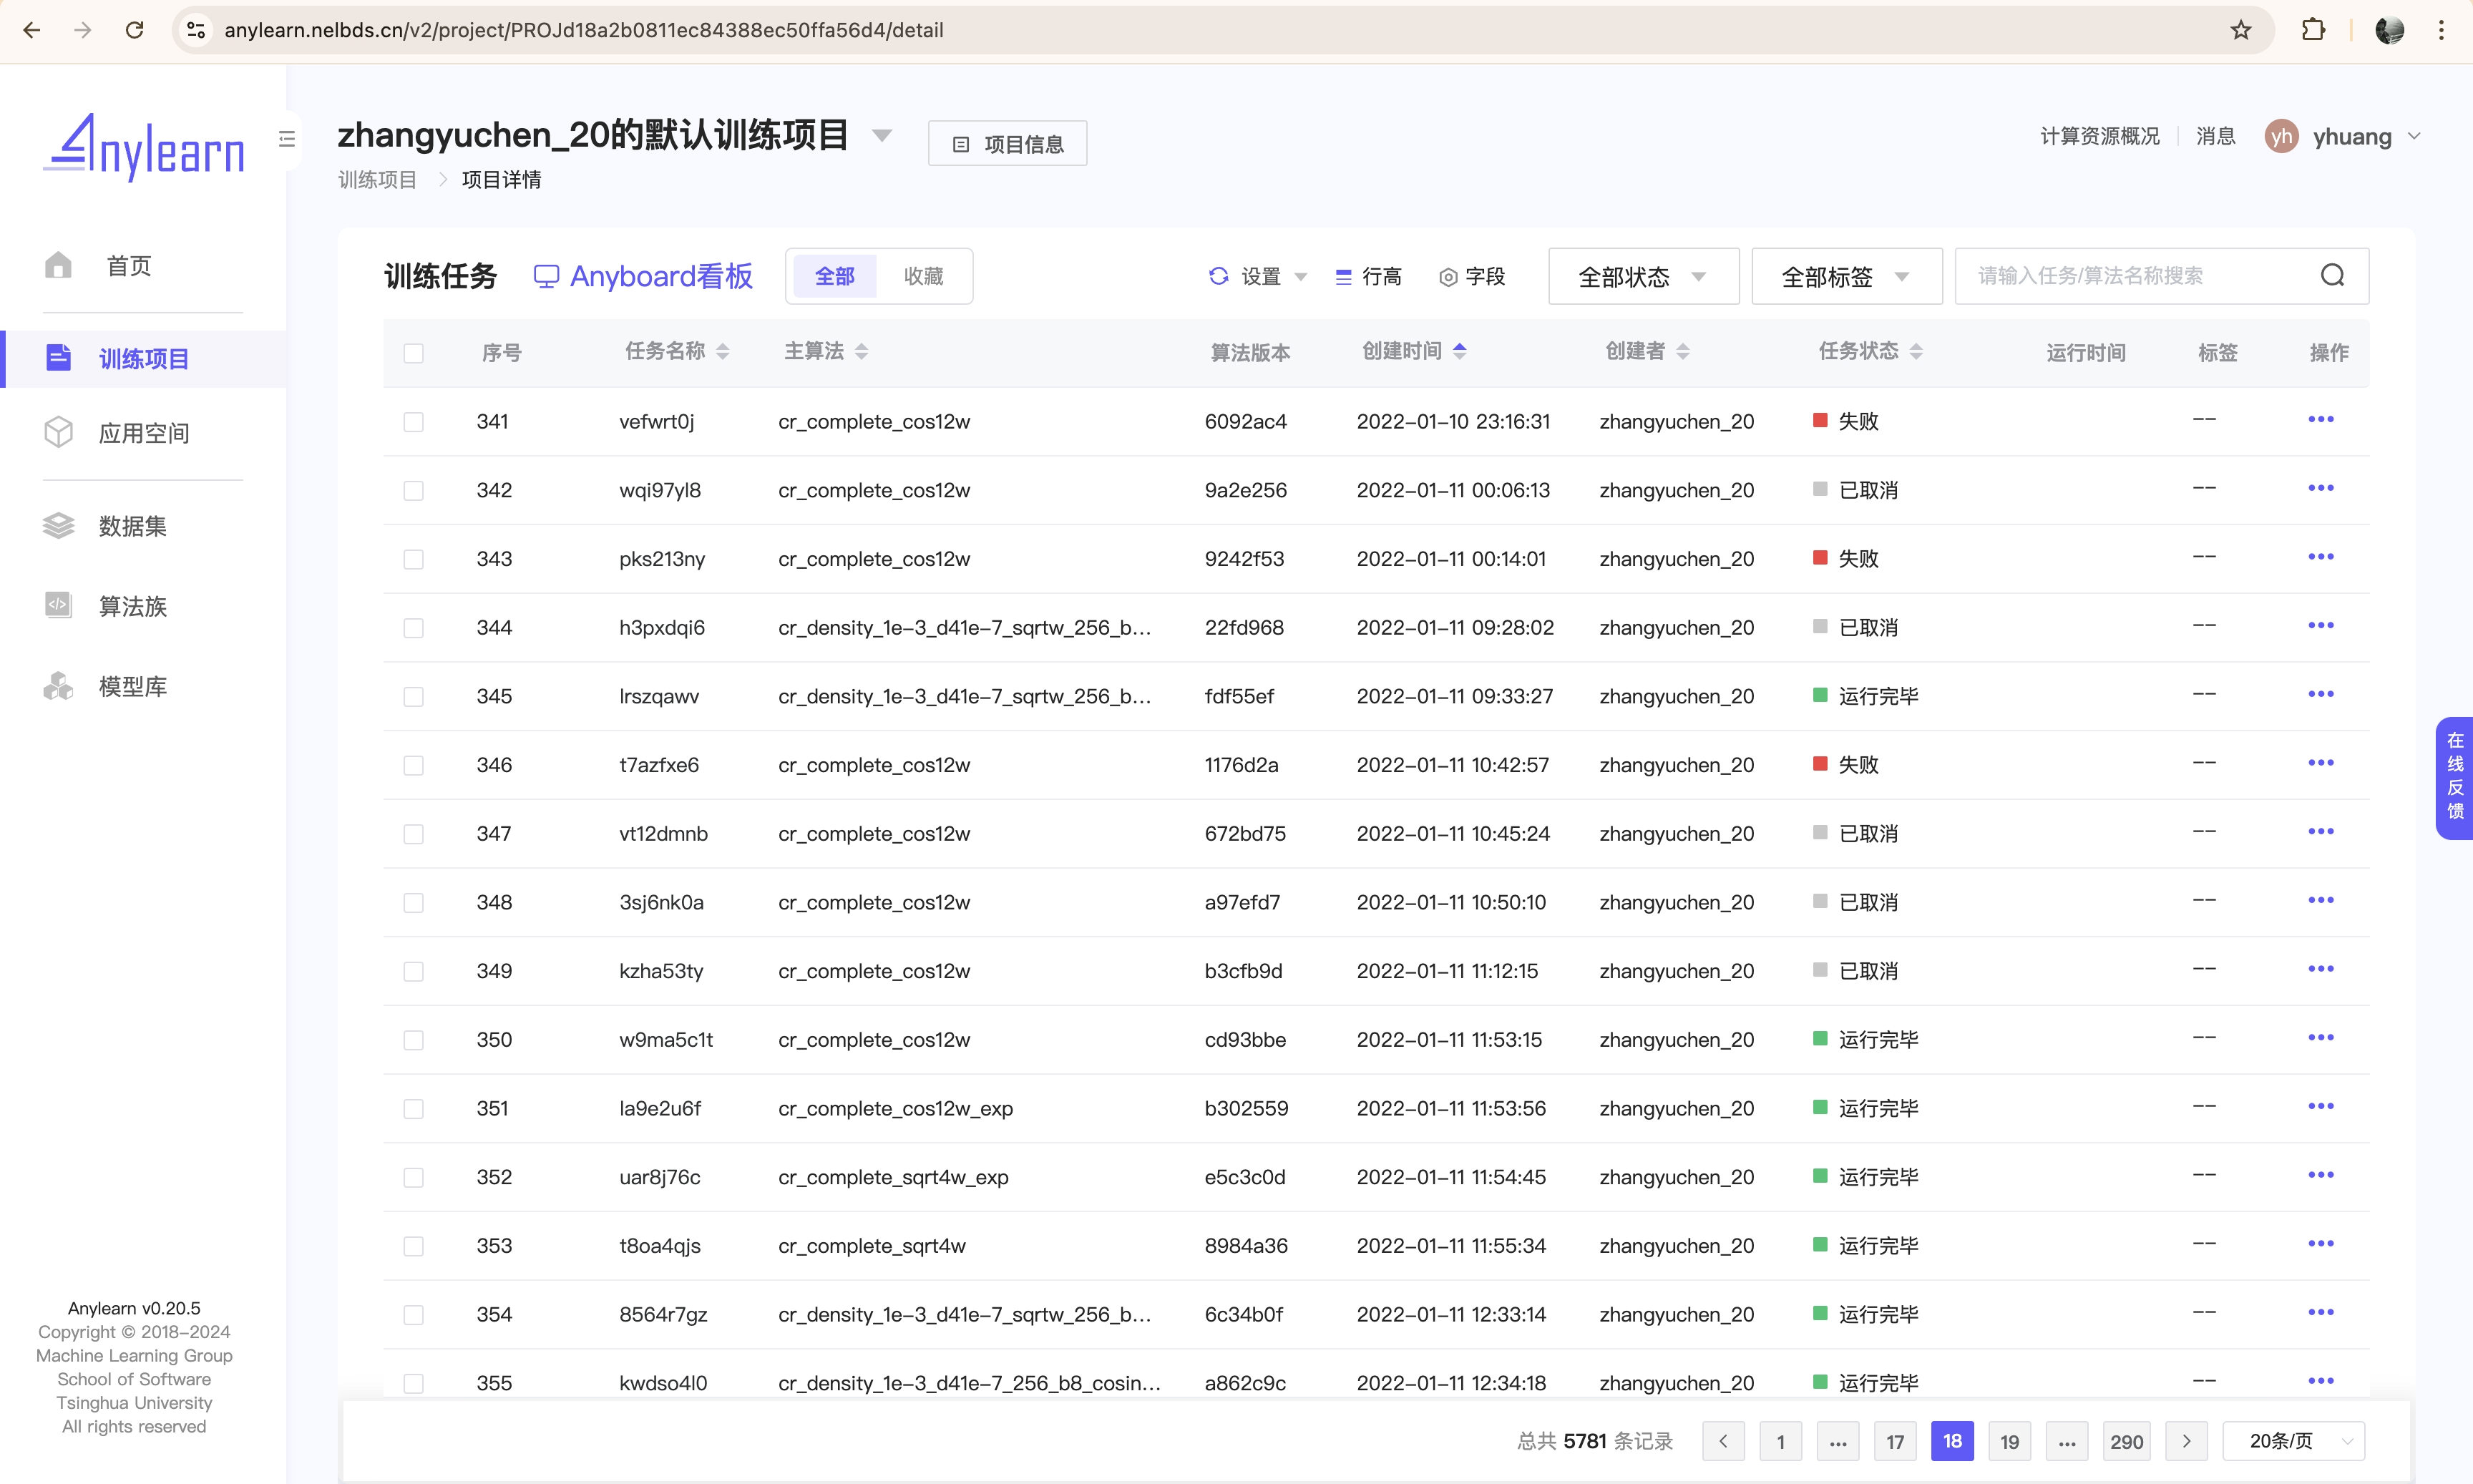
\includegraphics[width=0.98\linewidth]{radar-tasks.jpg}
  \caption{Anylearn中雷达回波外推模型研发相关的部分实验列表}
  \label{fig:radartasks}
\end{figure}

\subsection{模型效果预览}
目前学界和业界缺乏雷达回波外推的量化指标,对外推效果的评定往往依赖于肉眼观察雷达云图。
因此,在雷达回波外推模型的研发过程中,研究人员需要大量地生成模型预测出的雷达云图并评价其效果。

\begin{figure}
  \centering
  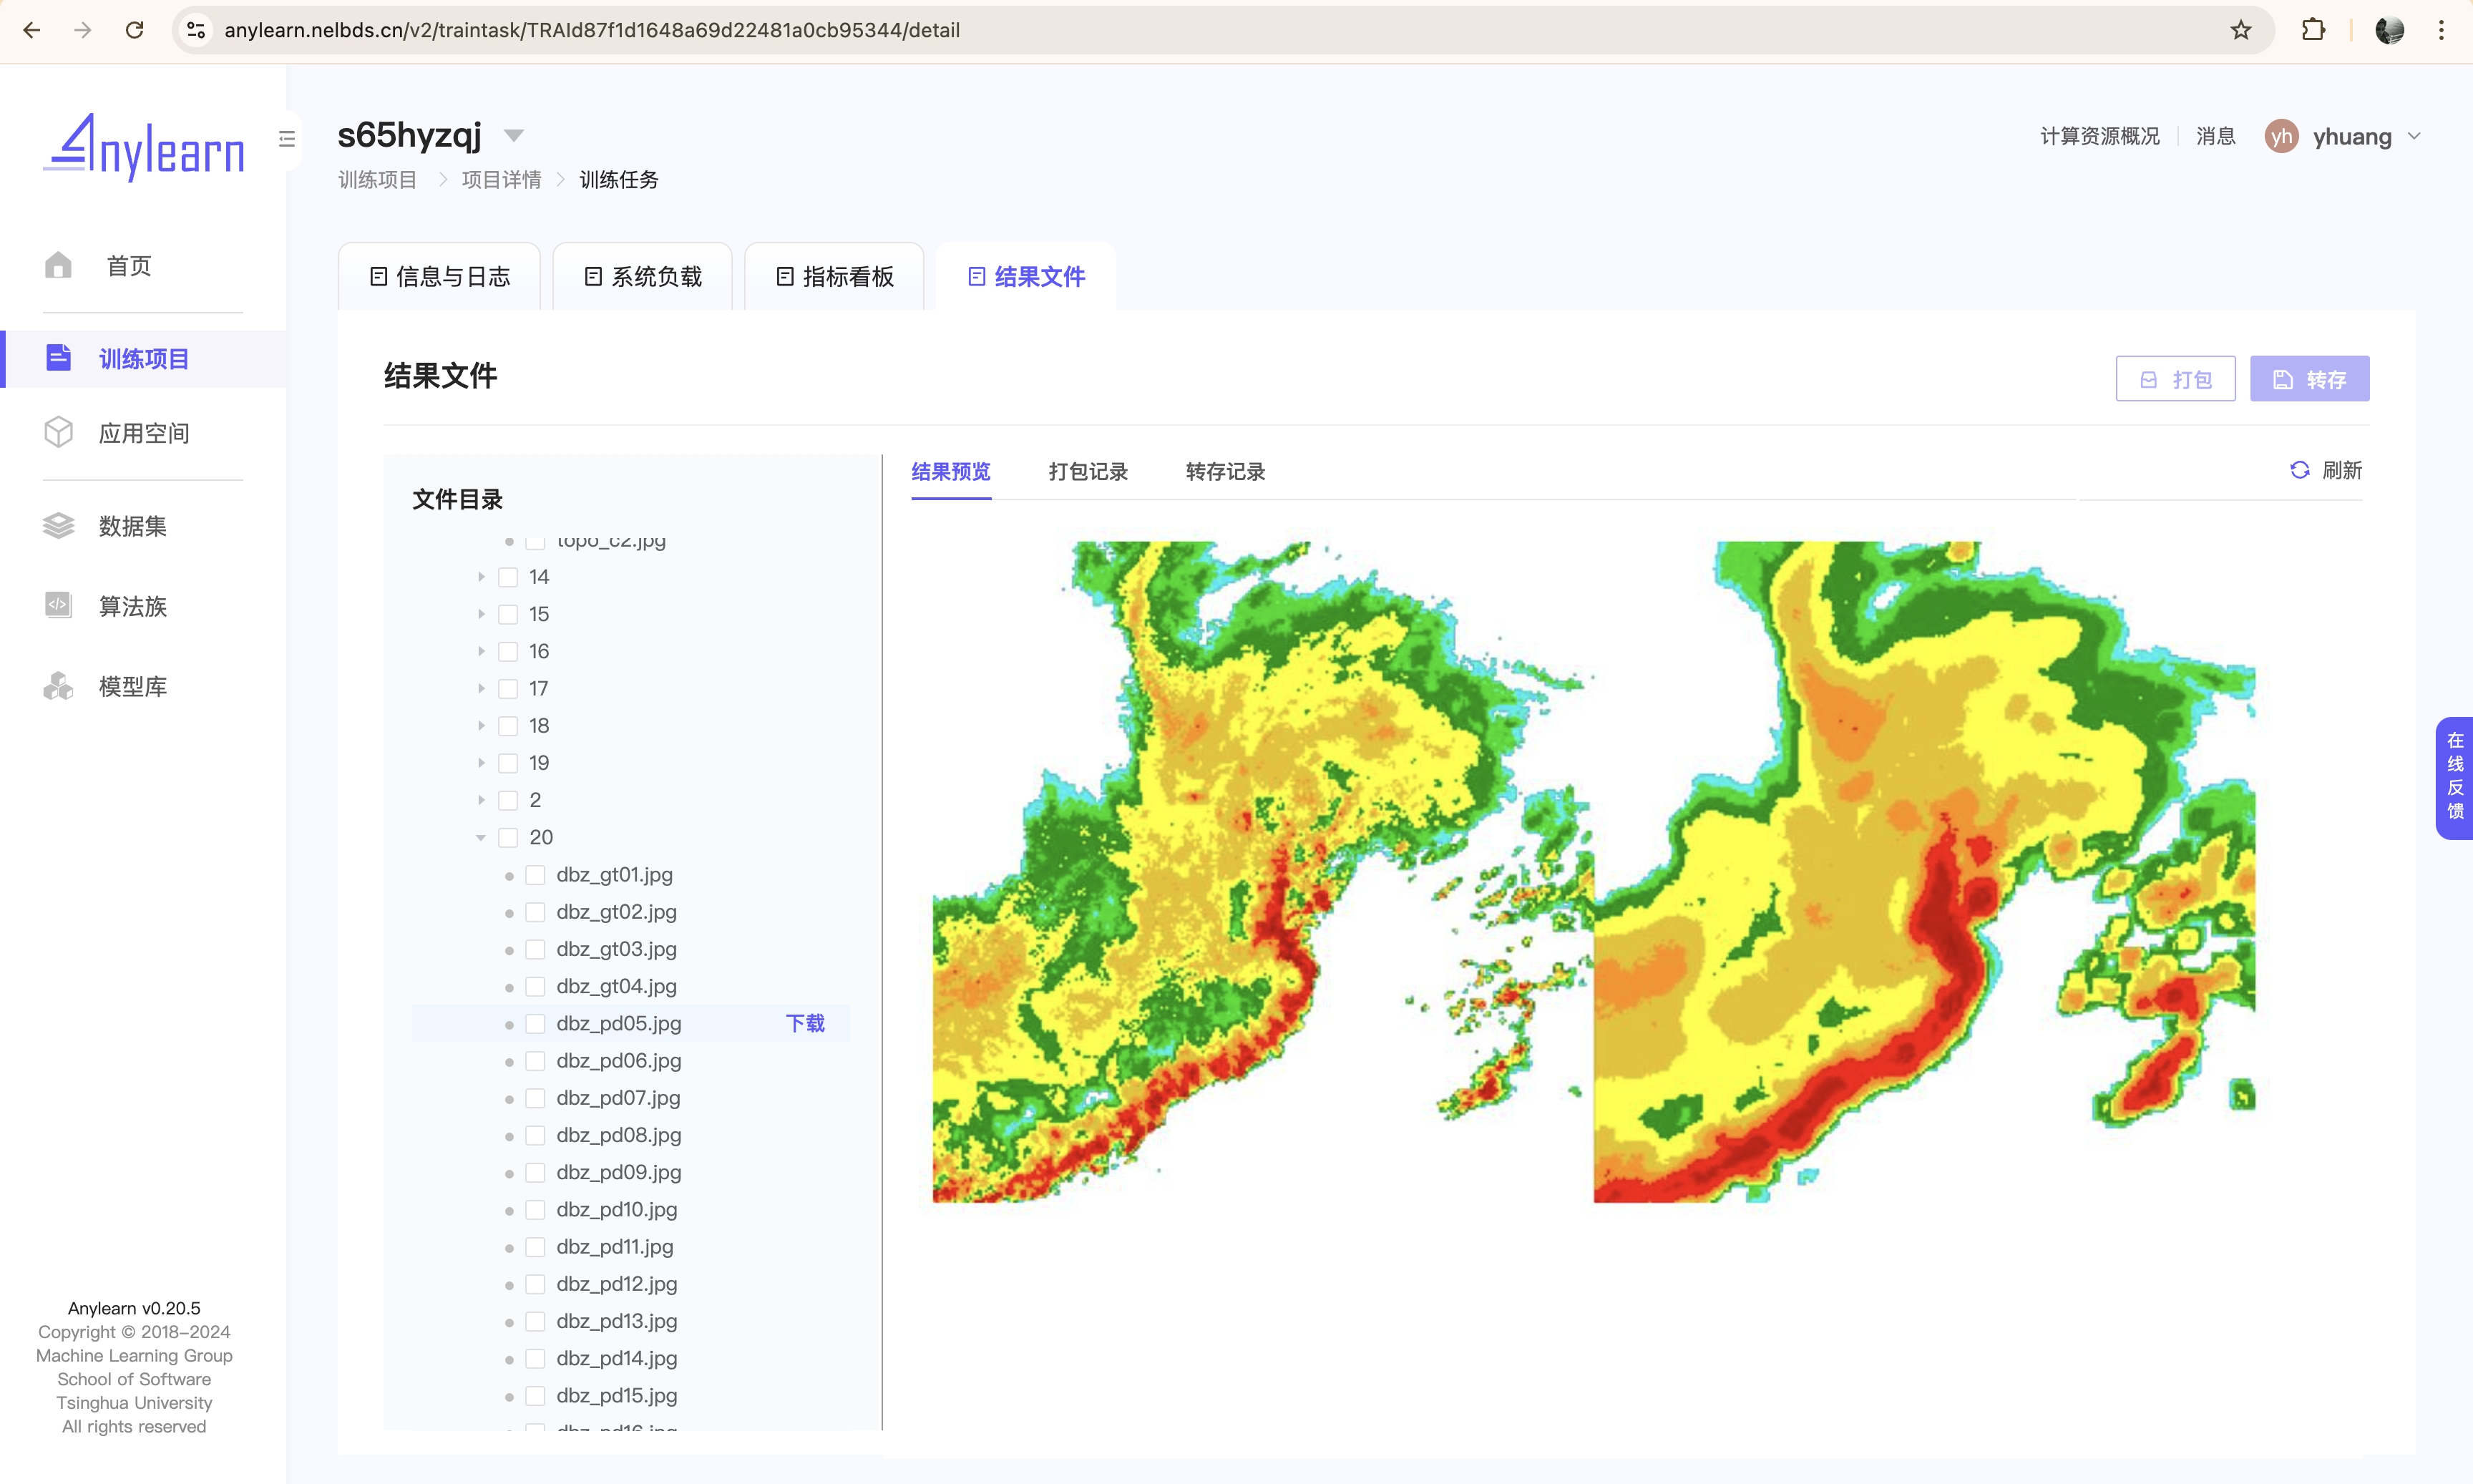
\includegraphics[width=0.98\linewidth]{radar-results.jpg}
  \caption{Anylearn中雷达回波外推实验结果可视化示例}
  \label{fig:radarresults}
\end{figure}

在未使用Anylearn之前,研究人员需要人工管理生成出的海量结果图片,并且经常需要将体积庞大的结果图包下载至个人电脑上进行查看。
而Anylearn能够自动地持久化每一次实验的结果文件,并原生支持在线查看图片类的结果文件,无需下载,完整覆盖了雷达回波外推模型评价的这一关键环节,如图\ref{fig:radarresults}所示。
此外,在雷达回波外推模型研发的后期需要专业气象预报专家在第三方系统中评测模型的效果,而Anylearn支持批量打包导出实验结果文件,有效地支撑了专家评测。

% !TeX root = ../thuthesis-example.tex

\chapter{总结与展望}

本文系统研究了云原生机器学习平台的体系架构、关键技术以及真实系统的设计实现。
针对机器学习研发中存在的流程缺乏顶层设计、资产缺乏统一管理、协作缺乏基础手段等挑战,本文提出了一个从能力、功能、数据、技术到交互的完整体系框架。
围绕平台的核心功能,本文研究了云原生系统和机器学习两方面的关键技术,包括容器化任务执行、资源池化调度、分布式存储管理、分布式训练、超参数调优、模型微调、模型更新等方面。
在此基础上,本文描述了真实的大数据机器学习研发管理系统Anylearn的设计实现和线上环境的应用情况,展示了平台在提升研发协作、资源利用率和实验复现性方面的显著成效,并证明其在真实的模型研发场景中的适用性和有效性。

未来的研究工作将围绕以下几个方向展开。

(1)国产化适配。
在全球人工智能战略布局的博弈中,国外软硬件生态对我国人工智能技术发展的封锁是当前人工智能领域最重大的风险点之一,卡脖子现象频发,国产化自主可控的人工智能软硬件生态则是破局的关键。
当前的云原生机器学习平台中的技术栈大多基于开源生态和国外算力基础设施,集成化的平台对于国产化软硬件的适配性有待充分验证。
Anylearn的国产化适配也是未来的重要工作之一。

(2)模型安全。
随着人工智能技术的广泛应用,模型安全问题日益凸显,如对抗攻击、隐私泄露、模型解释性等问题。
未来的研究也需要重点围绕模型安全展开,包括对抗攻击下的模型鲁棒性、隐私保护下的模型训练、模型解释性等方面。

(3)大模型底座。
自2022年底,大语言模型经历了爆炸式的增长,同时也带动了广泛意义上大模型技术的发展,如气象大模型、时序大模型等。
随着规模化效应的加剧,机器学习研发在大模型时代面临的挑战将更加复杂。
如何通过机器学习平台来支撑大模型的研发、形成大模型底座,将是未来长期的研究重点。



% 其他部分
\backmatter

% 参考文献
\bibliography{ref/refs}  % 参考文献使用 BibTeX 编译
% \printbibliography       % 参考文献使用 BibLaTeX 编译

% 附录
% 本科生需要将附录放到声明之后,个人简历之前
\appendix
% % !TeX root = ../thuthesis-example.tex

\begin{survey}
\label{cha:survey}

\title{Title of the Survey}
\maketitle


\tableofcontents


本科生的外文资料调研阅读报告。


\section{Figures and Tables}

\subsection{Figures}

An example figure in appendix (Figure~\ref{fig:appendix-survey-figure}).

\begin{figure}
  \centering
  \includegraphics[width=0.6\linewidth]{example-image-a.pdf}
  \caption{Example figure in appendix}
  \label{fig:appendix-survey-figure}
\end{figure}


\subsection{Tables}

An example table in appendix (Table~\ref{tab:appendix-survey-table}).

\begin{table}
  \centering
  \caption{Example table in appendix}
  \begin{tabular}{ll}
    \toprule
    File name       & Description                                         \\
    \midrule
    thuthesis.dtx   & The source file including documentation and comments \\
    thuthesis.cls   & The template file                                   \\
    thuthesis-*.bst & BibTeX styles                                       \\
    thuthesis-*.bbx & BibLaTeX styles for bibliographies                  \\
    thuthesis-*.cbx & BibLaTeX styles for citations                       \\
    \bottomrule
  \end{tabular}
  \label{tab:appendix-survey-table}
\end{table}


\section{Equations}

An example equation in appendix (Equation~\eqref{eq:appendix-survey-equation}).
\begin{equation}
  \frac{1}{2 \uppi \symup{i}} \int_\gamma f = \sum_{k=1}^m n(\gamma; a_k) \mathscr{R}(f; a_k)
  \label{eq:appendix-survey-equation}
\end{equation}


\section{Citations}

Example\cite{dupont1974bone} citations\cite{merkt1995rotational} in appendix
\cite{dupont1974bone,merkt1995rotational}.


% 默认使用正文的参考文献样式;
% 如果使用 BibTeX,可以切换为其他兼容 natbib 的 BibTeX 样式。
\bibliographystyle{unsrtnat}
% \bibliographystyle{IEEEtranN}

% 默认使用正文的参考文献 .bib 数据库;
% 如果使用 BibTeX,可以改为指定数据库,如 \bibliography{ref/refs}。
\printbibliography

\end{survey}
       % 本科生:外文资料的调研阅读报告
% % !TeX root = ../thuthesis-example.tex

\begin{translation}
\label{cha:translation}

\title{书面翻译题目}
\maketitle

\tableofcontents


本科生的外文资料书面翻译。


\section{图表示例}

\subsection{图}

附录中的图片示例(图~\ref{fig:appendix-translation-figure})。

\begin{figure}
  \centering
  \includegraphics[width=0.6\linewidth]{example-image-a.pdf}
  \caption{附录中的图片示例}
  \label{fig:appendix-translation-figure}
\end{figure}


\subsection{表格}

附录中的表格示例(表~\ref{tab:appendix-translation-table})。

\begin{table}
  \centering
  \caption{附录中的表格示例}
  \begin{tabular}{ll}
    \toprule
    文件名          & 描述                         \\
    \midrule
    thuthesis.dtx   & 模板的源文件,包括文档和注释 \\
    thuthesis.cls   & 模板文件                     \\
    thuthesis-*.bst & BibTeX 参考文献表样式文件    \\
    thuthesis-*.bbx & BibLaTeX 参考文献表样式文件  \\
    thuthesis-*.cbx & BibLaTeX 引用样式文件        \\
    \bottomrule
  \end{tabular}
  \label{tab:appendix-translation-table}
\end{table}


\section{数学公式}

附录中的数学公式示例(公式\eqref{eq:appendix-translation-equation})。
\begin{equation}
  \frac{1}{2 \uppi \symup{i}} \int_\gamma f = \sum_{k=1}^m n(\gamma; a_k) \mathscr{R}(f; a_k)
  \label{eq:appendix-translation-equation}
\end{equation}


\section{文献引用}

附录\cite{dupont1974bone}中的参考文献引用\cite{merkt1995rotational}示例
\cite{dupont1974bone,merkt1995rotational}。


\appendix

\section{附录}

附录的内容。


% 书面翻译的参考文献
% 默认使用正文的参考文献样式;
% 如果使用 BibTeX,可以切换为其他兼容 natbib 的 BibTeX 样式。
\bibliographystyle{unsrtnat}
% \bibliographystyle{IEEEtranN}

% 默认使用正文的参考文献 .bib 数据库;
% 如果使用 BibTeX,可以改为指定数据库,如 \bibliography{ref/refs}。
\printbibliography

% 书面翻译对应的原文索引
\begin{translation-index}
  \nocite{mellinger1996laser}
  \nocite{bixon1996dynamics}
  \nocite{carlson1981two}
  \bibliographystyle{unsrtnat}
  \printbibliography
\end{translation-index}

\end{translation}
  % 本科生:外文资料的书面翻译
% !TeX root = ../thuthesis-example.tex

\chapter{Anylearn功能设计详情}

TBD


% 致谢
% !TeX root = ../thuthesis-example.tex

\begin{acknowledgements}
  衷心感谢我的合作导师王建民教授的谆谆教诲。是王老师在系统设计和工程应用方面对我的言传身教,使我对工业大数据和人工智能领域的系统软件工程有了更为深刻的理解。

  特别感谢龙明盛副教授在机器学习技术和系统方面的指导,带领我深入研究机器学习系统,帮助我在人工智能工程化的道路上前行。

  博士后期间的工作有诸多挑战,感谢裴忠一、乔嘉林、王彦凯等博士后师兄弟的帮助,与你们共度在校生活是我的荣幸。
  感谢我云原生技术的领路人、共事颇短但终成莫逆的黄超,感谢王团团工程师、岑知遥等Anylearn小组的伙伴,感谢我们一起追逐过的梦想。
  也真心感谢张育宸、邢蓝翔、吴佳龙、董家祥、吴海旭等实验室同学们的支持,是你们督促着我不断进步。
  
  最后还要感谢我的家人和朋友们。
  感谢我的父母,感谢你们传授于我的工作经验和人生哲学,是你们让我成为了今天的自己。
  感谢我的挚友李唯和卞可欣,感谢你们在我迷茫时的鼓励。
  感谢我的至交高凌宇,我们灵魂的碰撞是我这几年最坚实的精神支柱。
  感谢我的爱人逸鹤、爱子瑞泽、爱猫鱼头,感谢你在风浪中给予我的陪伴,你们是我坚持下去的动力。

  终局未竞,也不忘感谢自己,虽非完人,但无愧于心。
\end{acknowledgements}


% 声明
% 本科生开题报告不需要
\statement
% 将签字扫描后的声明文件 scan-statement.pdf 替换原始页面
% \statement[file=scan-statement.pdf]
% 本科生编译生成的声明页默认不加页脚,插入扫描版时再补上;
% 研究生编译生成时有页眉页脚,插入扫描版时不再重复。
% 也可以手动控制是否加页眉页脚
% \statement[page-style=empty]
% \statement[file=scan-statement.pdf, page-style=plain]

% 个人简历、在学期间完成的相关学术成果
% 本科生可以附个人简历,也可以不附个人简历
% !TeX root = ../thuthesis-example.tex

\begin{resume}

  \section*{个人简历}

  1990 年 6 月 13 日出生于北京市海淀区。

  2009 年 2 月考入法国特鲁瓦技术大学计算机科学与信息系统专业,2014 年 7 月毕业并获得工程师学位(等同于硕士学位)。

  2013 年 9 月进入法国特鲁瓦技术大学系统优化与安全专业攻读硕士学位(双学位),2014 年 7 月毕业获得硕士学位。

  2015 年 3 月免试进入法国特鲁瓦技术大学系统优化与安全专业攻读博士学位,2018 年 6 月毕业获得博士学位。

  2018 年 9 月至 2020 年 7 月于 CGI 集团(法国)公司担任技术专家。

  2020 年 11 月作为博士后入职清华大学软件学院至今。


  \section*{博士后工作期间完成的相关学术成果}

  \subsection*{学术论文}

  \begin{achievements}
    \item Pei Z Y, Cen Z Y, \textbf{Huang Y P}, et al. BTTackler: A Diagnosis-based Framework for Efficient Deep Learning Hyperparameter Optimization[C]. In Proceedings of the 30th ACM SIGKDD Conference on Knowledge Discovery and Data Mining (KDD'24). Barcelona, Spain. 2024. (CCF-A, TH-CPL-A)
  \end{achievements}


  \subsection*{专利}

  \begin{achievements}
    \item 裴忠一, 岑知遥, \textbf{黄亦芃}, 等. 基于训练质量分析的超参数优化方法、装置及电子设备: 中国, CN117933370A[P]. 2024-04-26.
    \item 裴忠一, 陈俣策, \textbf{黄亦芃}, 等. 机器学习项目代码修改检测方法及装置: 中国, CN116860605A[P]. 2023-10-10.
  \end{achievements}

\end{resume}


% 指导教师/指导小组评语
% 本科生不需要
% \input{data/comments}

% 答辩委员会决议书
% 本科生不需要
% \input{data/resolution}

% 本科生的综合论文训练记录表(扫描版)
% \record{file=scan-record.pdf}

\end{document}
